\chapter{Basic user interface explanation}

\section{Icon meaning list}
\label{sec:icon_list}

The User Interface (UI) of ToM is really intuitive and easy to use, and each data is
represented with a specific icon which usually reminds what that data can be useful
for. Here is a list of all icons which you could find on the ToM and their meanings.

\subsection{Page icons}
\label{sec:page_icon_list}

Page icons are the icons which you can find on the bottom line of the ToM+ display
and they are used to switch between the different pages. Since the last update they
have been revamped with a 3D metallic look.

\iconbox{icons/BatteryV2.png}
{Battery page}
{Shows main values about the battery.}

\iconbox{icons/Motor.png}
{Engine page}
{Shows main values about the engine.}

\iconbox{icons/BatteryInfo2.png}
{Battery info page}
{Shows detailed information about battery cells.}

\iconbox{icons/Alarm.PNG}
{Alarm log page}
{Shows the list of last alarms triggers and their details.}

\iconbox{icons/Error.png}
{Error log page}
{Shows the list of last errors and their details.}

\iconbox{icons/TripLog.png}
{Trip log page}
{Shows the list of last trips and their details.}

\iconbox{icons/Gyroscope.png}
{Gyroscope page}
{Shows main values about the gyroscope and miscellaneous.}

\iconbox{icons/Street0Ok_v2.png}
{Trip page}
{Shows main values about the selected trip.}

\iconbox{icons/3Dots.PNG}
{Settings page}
{Shows various settings and options for the ToM+.}

\subsection{Battery group}
\label{sec:item_numbers}

\iconbox{icons/BatterySoc.jpg}
{(1) State Of Charge (\%)}
{The current state of charge of the battery.}

\iconbox{icons/BatterySoh.jpg}
{(2) State Of Health (\%)}
{The current state of health of the battery.}

\iconbox{icons/BatteryKwh.jpg}
{(6) Battery remaining capacity (\(kWh\))}
{The remaining energy stored in the battery.}

\iconbox{icons/BatteryA.jpg}
{(7) Battery instant current consumption (\(A\))}
{The current flowing through the battery.}

\iconbox{icons/BatteryA+red.png}
{(7) Battery current recharge (\(A\))}
{The current recharge by regenerative braking.}

\iconbox{icons/BatteryKw.png}
{(54) Battery instant power (\(kW\))}
{The power flowing through the battery.}

\iconbox{icons/Battery3°.jpg}
{(3) Battery temperature (\textdegree~C)}
{The current temperature of the battery.}

\iconbox{icons/BatteryV2.jpg}
{(25) Battery voltage (\(V\))}
{The current voltage of the traction battery.}

\iconbox{icons/BatteryV.jpg}
{(39) 12V battery voltage (\(V\))}
{The current voltage of the 12V battery.}

\iconbox{icons/BatteryDiff.png}
{(5) Min-Max battery cell difference (\(V\))}
{The difference between the minimum and maximum battery cell voltages.}

\subsection{Charging group}

\iconbox{icons/CEta.png}
{(55) Charging ETA (\(min\))}
{The estimated time remaining for the battery to be fully charged.}

\iconbox{icons/Charge°.png}
{(57) Charger temperature (\textdegree~C)}
{The current temperature of the charger.}

\iconbox{icons/ChargedKwh.png}
{(56) Charged energy (\(kWh\))}
{The amount of energy that has been charged into the battery.}

\iconbox{icons/ChargeKwh.png}
{(58) Instant charging power (\(kW\))}
{The current power being delivered to the battery.}

\subsection{Motor group}

\iconbox{icons/MotoRPM2.jpg}
{(8) Motor RPM (\(rpm\))}
{The current revolutions per minute of the motor.}

\iconbox{icons/MotorNm.jpg}
{(9) Motor torque (\(Nm\))}
{The current torque being produced by the motor.}

\iconbox{icons/Motor°2.jpg}
{(4) Motor temperature (\textdegree~C)}
{The current temperature of the motor.}

\iconbox{icons/Sev°.png}
{(45) Sevcon temperature (\textdegree~C)}
{The current temperature of the Sevcon controller.}

\subsection{Expansion port group}

\iconbox{icons/Pin1.png}
{(40) Expansion port PIN1 (\(0/1\))}
{The binary state of the expansion port PIN1.}

\iconbox{icons/Pin2.png}
{(41) Expansion port PIN2 (\(0/1\))}
{The binary state of the expansion port PIN2.}

\subsection{Gyroscope group}

\iconbox{icons/InclDX.PNG}
{(62) Gyroscope right X-axis (\textdegree)}
{The current right angle of the gyroscope along the X-axis.}

\iconbox{icons/InclSX.PNG}
{(62) Gyroscope left X-axis (\textdegree)}
{The current left angle of the gyroscope along the X-axis.}

\iconbox{icons/UphillTwizy.png}
{(63) Frontal uphill inclination (\textdegree)}
{The current frontal uphill angle of the gyroscope.}

\iconbox{icons/DownhillTwizy.png}
{(63) Frontal downhill inclination (\textdegree)}
{The current frontal downhill angle of the gyroscope.}

\iconbox{icons/GyroAcc.JPG}
{(61) Gyroscope acceleration (\(m/s^2\))}
{The current car acceleration measured by the gyroscope.}

\iconbox{icons/Gtemp.PNG}
{(60) ToM+ black box temperature (\textdegree~C)}
{The current temperature of the ToM+ black box.}

\iconbox{icons/Timer.PNG}
{(59) Time elapsed (\(min\))}
{The current time elapsed from power on.}

\subsection{Trip group}

\iconbox{icons/tKm.png}
{(46) Trip distance (\(km\))}
{The current distance traveled in the current trip.}

\iconbox{icons/tKmh.png}
{(53) Trip average speed (\(km/h\))}
{The current average speed in the current trip.}

\iconbox{icons/tKmR.png}
{(47) Trip kilometers left (\(km\))}
{The remaining kilometer range with the current trip consumption.}

\iconbox{icons/tkWh.png}
{(49) Trip total power consumption (\(kWh\))}
{The total power consumption in the current trip.}

\iconbox{icons/tkWh100.png}
{(50) Trip power consumption per 100 kilometers (\(kWh/100km\))}
{The current power consumption per 100 kilometers in the current trip.}

\iconbox{icons/tkWh1min.png}
{(52) Trip power consumption per minute (\(kWh/min\))}
{The current power consumption per minute in the current trip.}

\iconbox{icons/tTimer.png}
{(48) Trip time (\(min\))}
{The current time elapsed in the current trip.}

\iconbox{icons/tUphill.png}
{(38) Trip uphill average inclination (\textdegree)}
{The average uphill inclination in the current trip.}

\iconbox{icons/tDownhill.png}
{(38) Trip downhill average inclination (\textdegree)}
{The average downhill inclination in the current trip.}

\subsection{Dashboard group}

\iconbox{icons/ODO.png}
{(42) Odometer (\(km\))}
{The total distance traveled by the vehicle.}

\iconbox{icons/Kmh.png}
{Current speed (\(km/h\))}
{(44) The current speed of the vehicle.}

\iconbox{icons/KmhR.png}
{(43) Kilometers left (\(km\))}
{The remaining distance calculated by the original dashboard.}

\iconbox{icons/KmRCalc.png}
{(51) Calculated kilometers left (\(km\))}
{The km left calculated by the ToM+ with customizable weighted average.}
\label{fig:calculated_kilometers_left}

\clearpage

\section{Dashboard page}

This section will cover the explanation of the dashboard page, which is the main
page of the ToM+, so probably the one you will use the most. In the image below
I have numbered the most important parts and I will explain each of them in the
following paragraphs.

\begin{figure}[H]
    \centering
    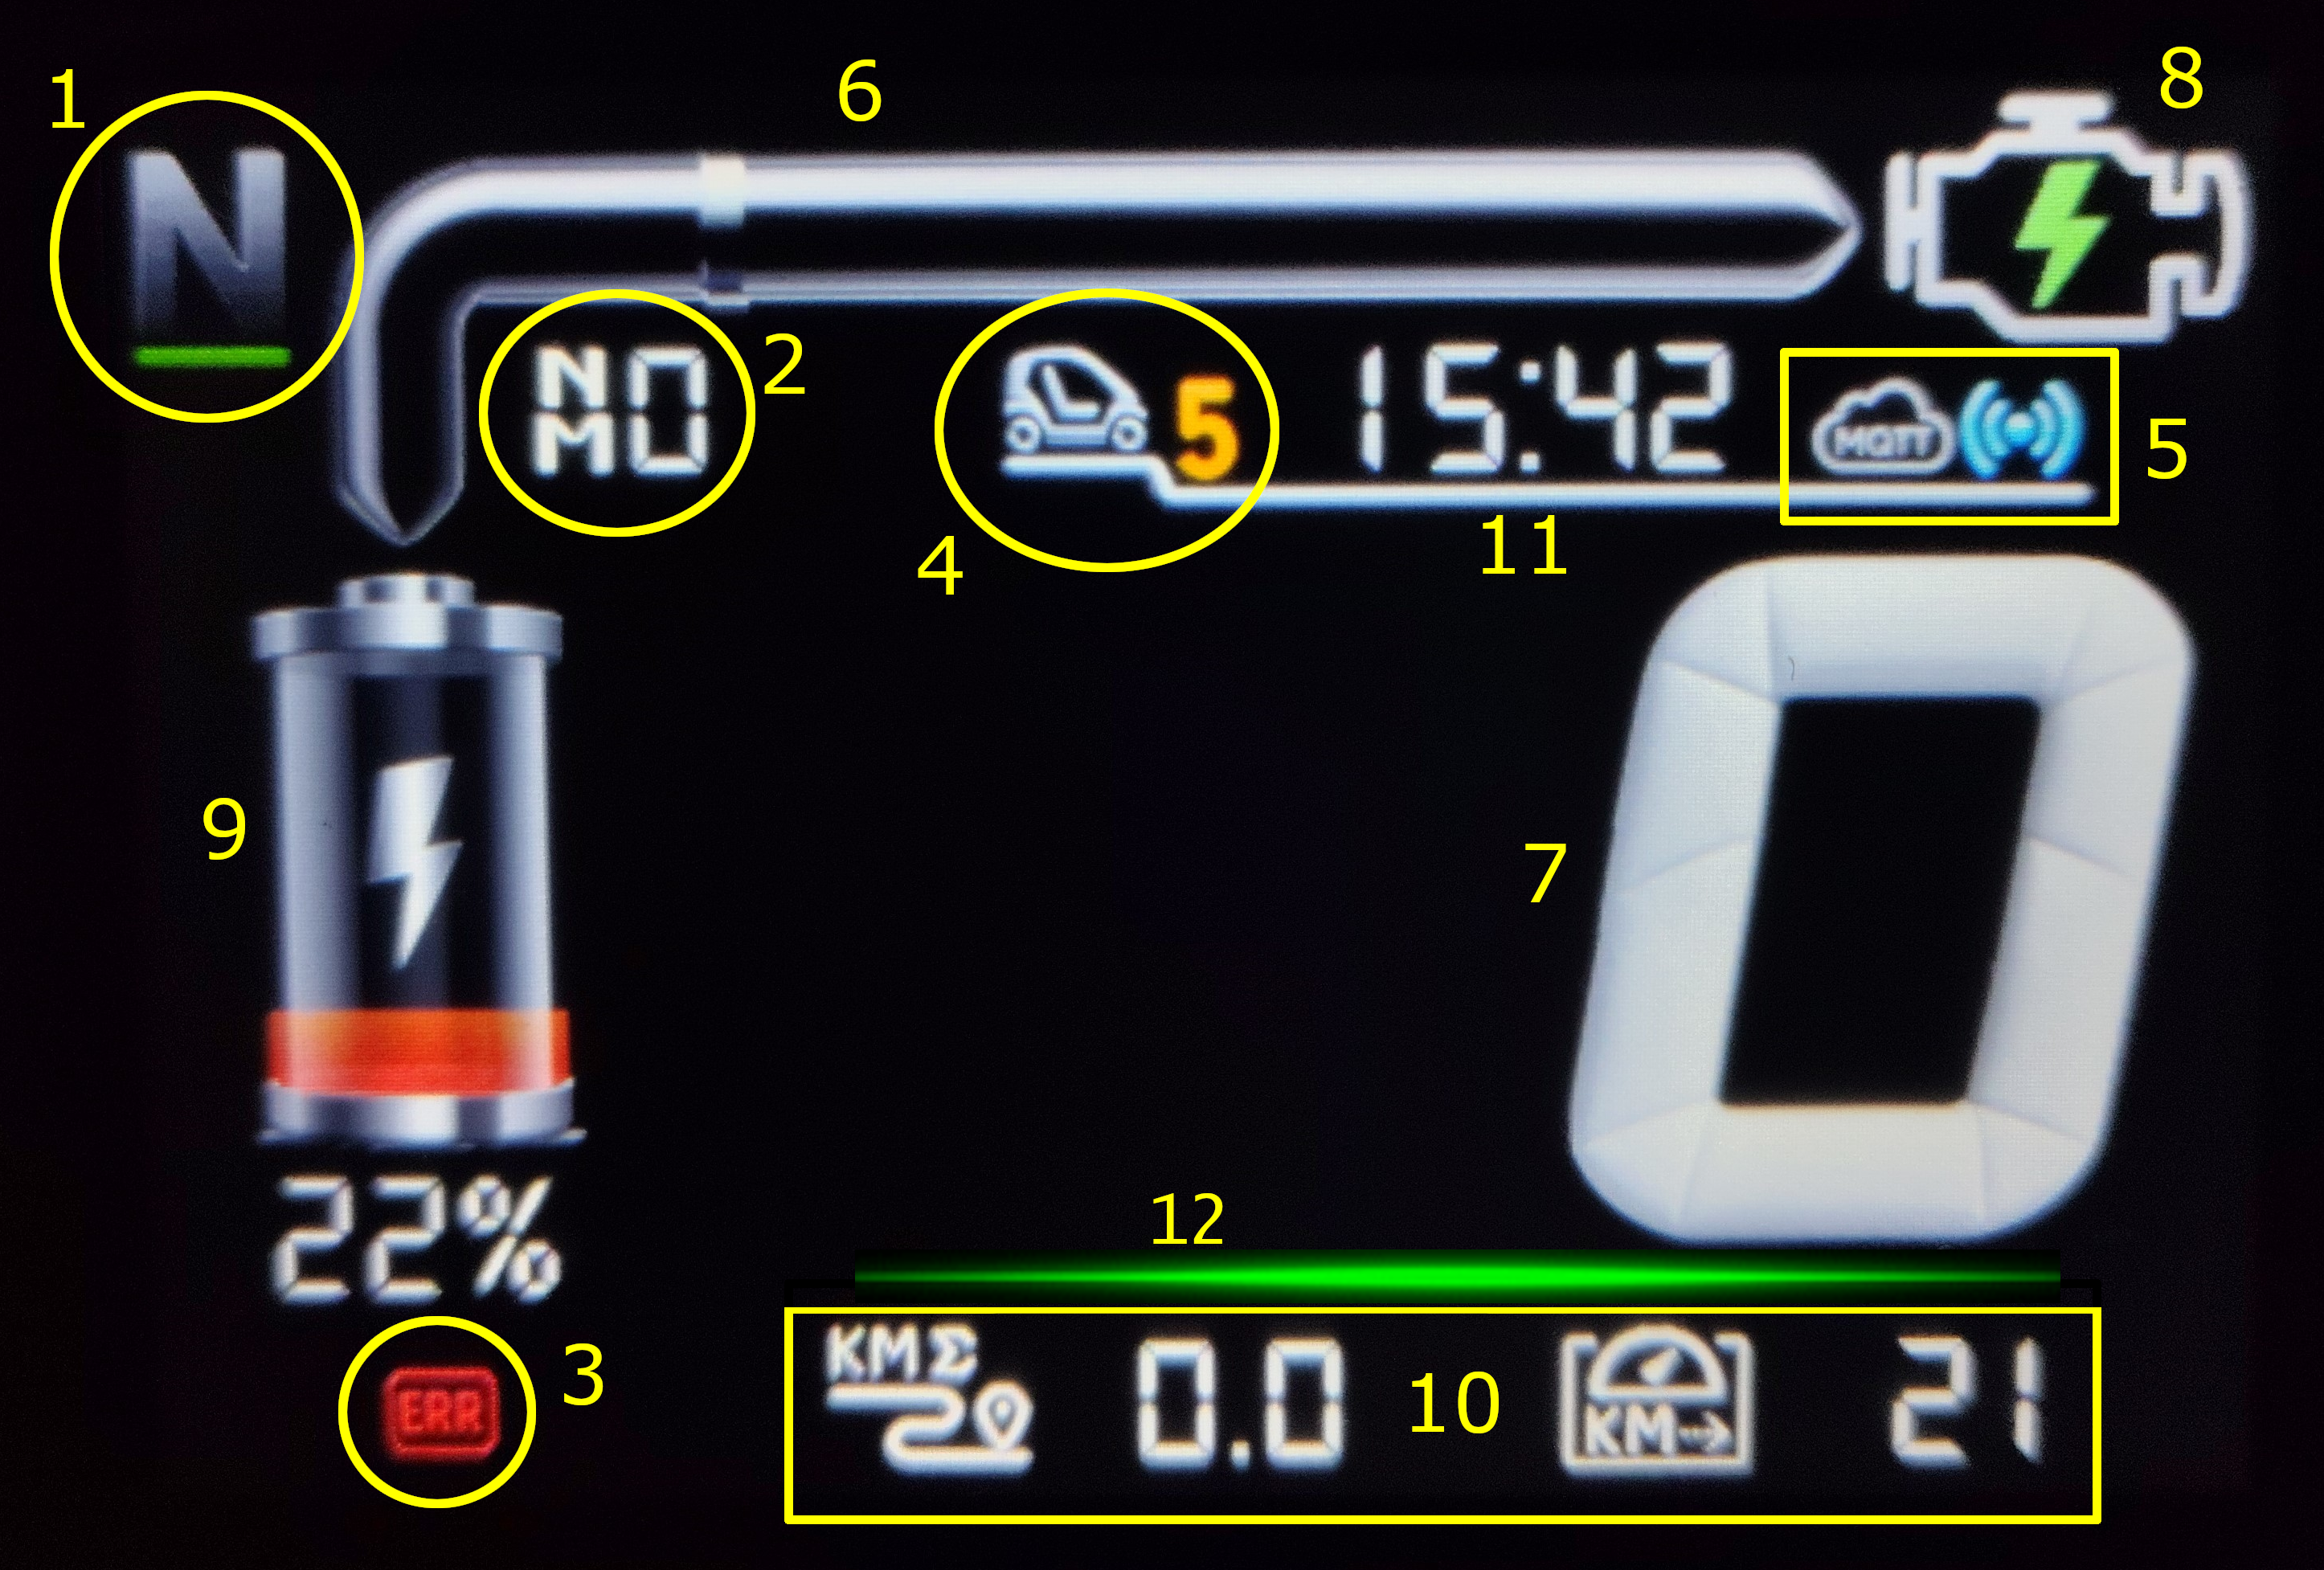
\includegraphics[width=0.8\textwidth]{figures/dashboard_numbers.PNG}
    \caption{Dashboard page with numbered parts.} \label{fig:dashboard_layout}
\end{figure}

\begin{description}
\item[\textbf{1}] Current gear of the vehicle, which is usually displayed on the original dashboard as well.
\item[\textbf{2}] A value chosen from torque, power consumption and current consumption, which is used to fill
the power bar described in item 6. Tap on the value to cycle between the three options.
\item[\textbf{3}] Error status icon, displayed when an error is present.
\item[\textbf{4}] Shows the active trip. Tap on the icon to open the trip page.
\item[\textbf{5}] Icons for MQTT and WiFi. Greyed out when disconnected, and colored when connected. Tap on the icons if you want to perform a new WiFi scan or a MQTT reconnection.
\item[\textbf{6}] Power bar displaying the selected value from item 2. Starting from the center line, the bar 
is filled from left to right when accelerating, and from right to left when in regenerative braking. 
The bar is filled with a color gradient in each direction, and the \textbf{maximum and minimum values are customizable} in the web server BigToM page.
\item[\textbf{7}] Displays the instant speed of the vehicle. You can choose between km/h and mph in the web server Advanced Info and Settings page.
\item[\textbf{8}] Motor icon, tap on it to open the motor page.
\item[\textbf{9}] Battery gradient colored icon, tap on it to open the battery info page.
\item[\textbf{10}] Additional displayed values, you can cycle between them by tapping on the icon to change.
\item[\textbf{11}] Displays the time and date, cycle between them by tapping on it.
\item[\textbf{12}] Customizable speed alert limit (green, yellow or red), see Section~\ref{sec:web_btom_tom_sets} to enable.
\end{description}

\section{The pages layout}
\label{sec:main-layout}

The layout can be divided in two main parts, that
we will see in detail in the next two paragraphs. The first is the data monitor which
has some features to change the data shown in foreground choosing from the ones
listed in the side bar. The second is the status icon bar, usually in the bottom of the page.
The battery, motor, gyroscope and trip pages share the same layout, shown in the picture.

\begin{figure}[H]
    \centering
    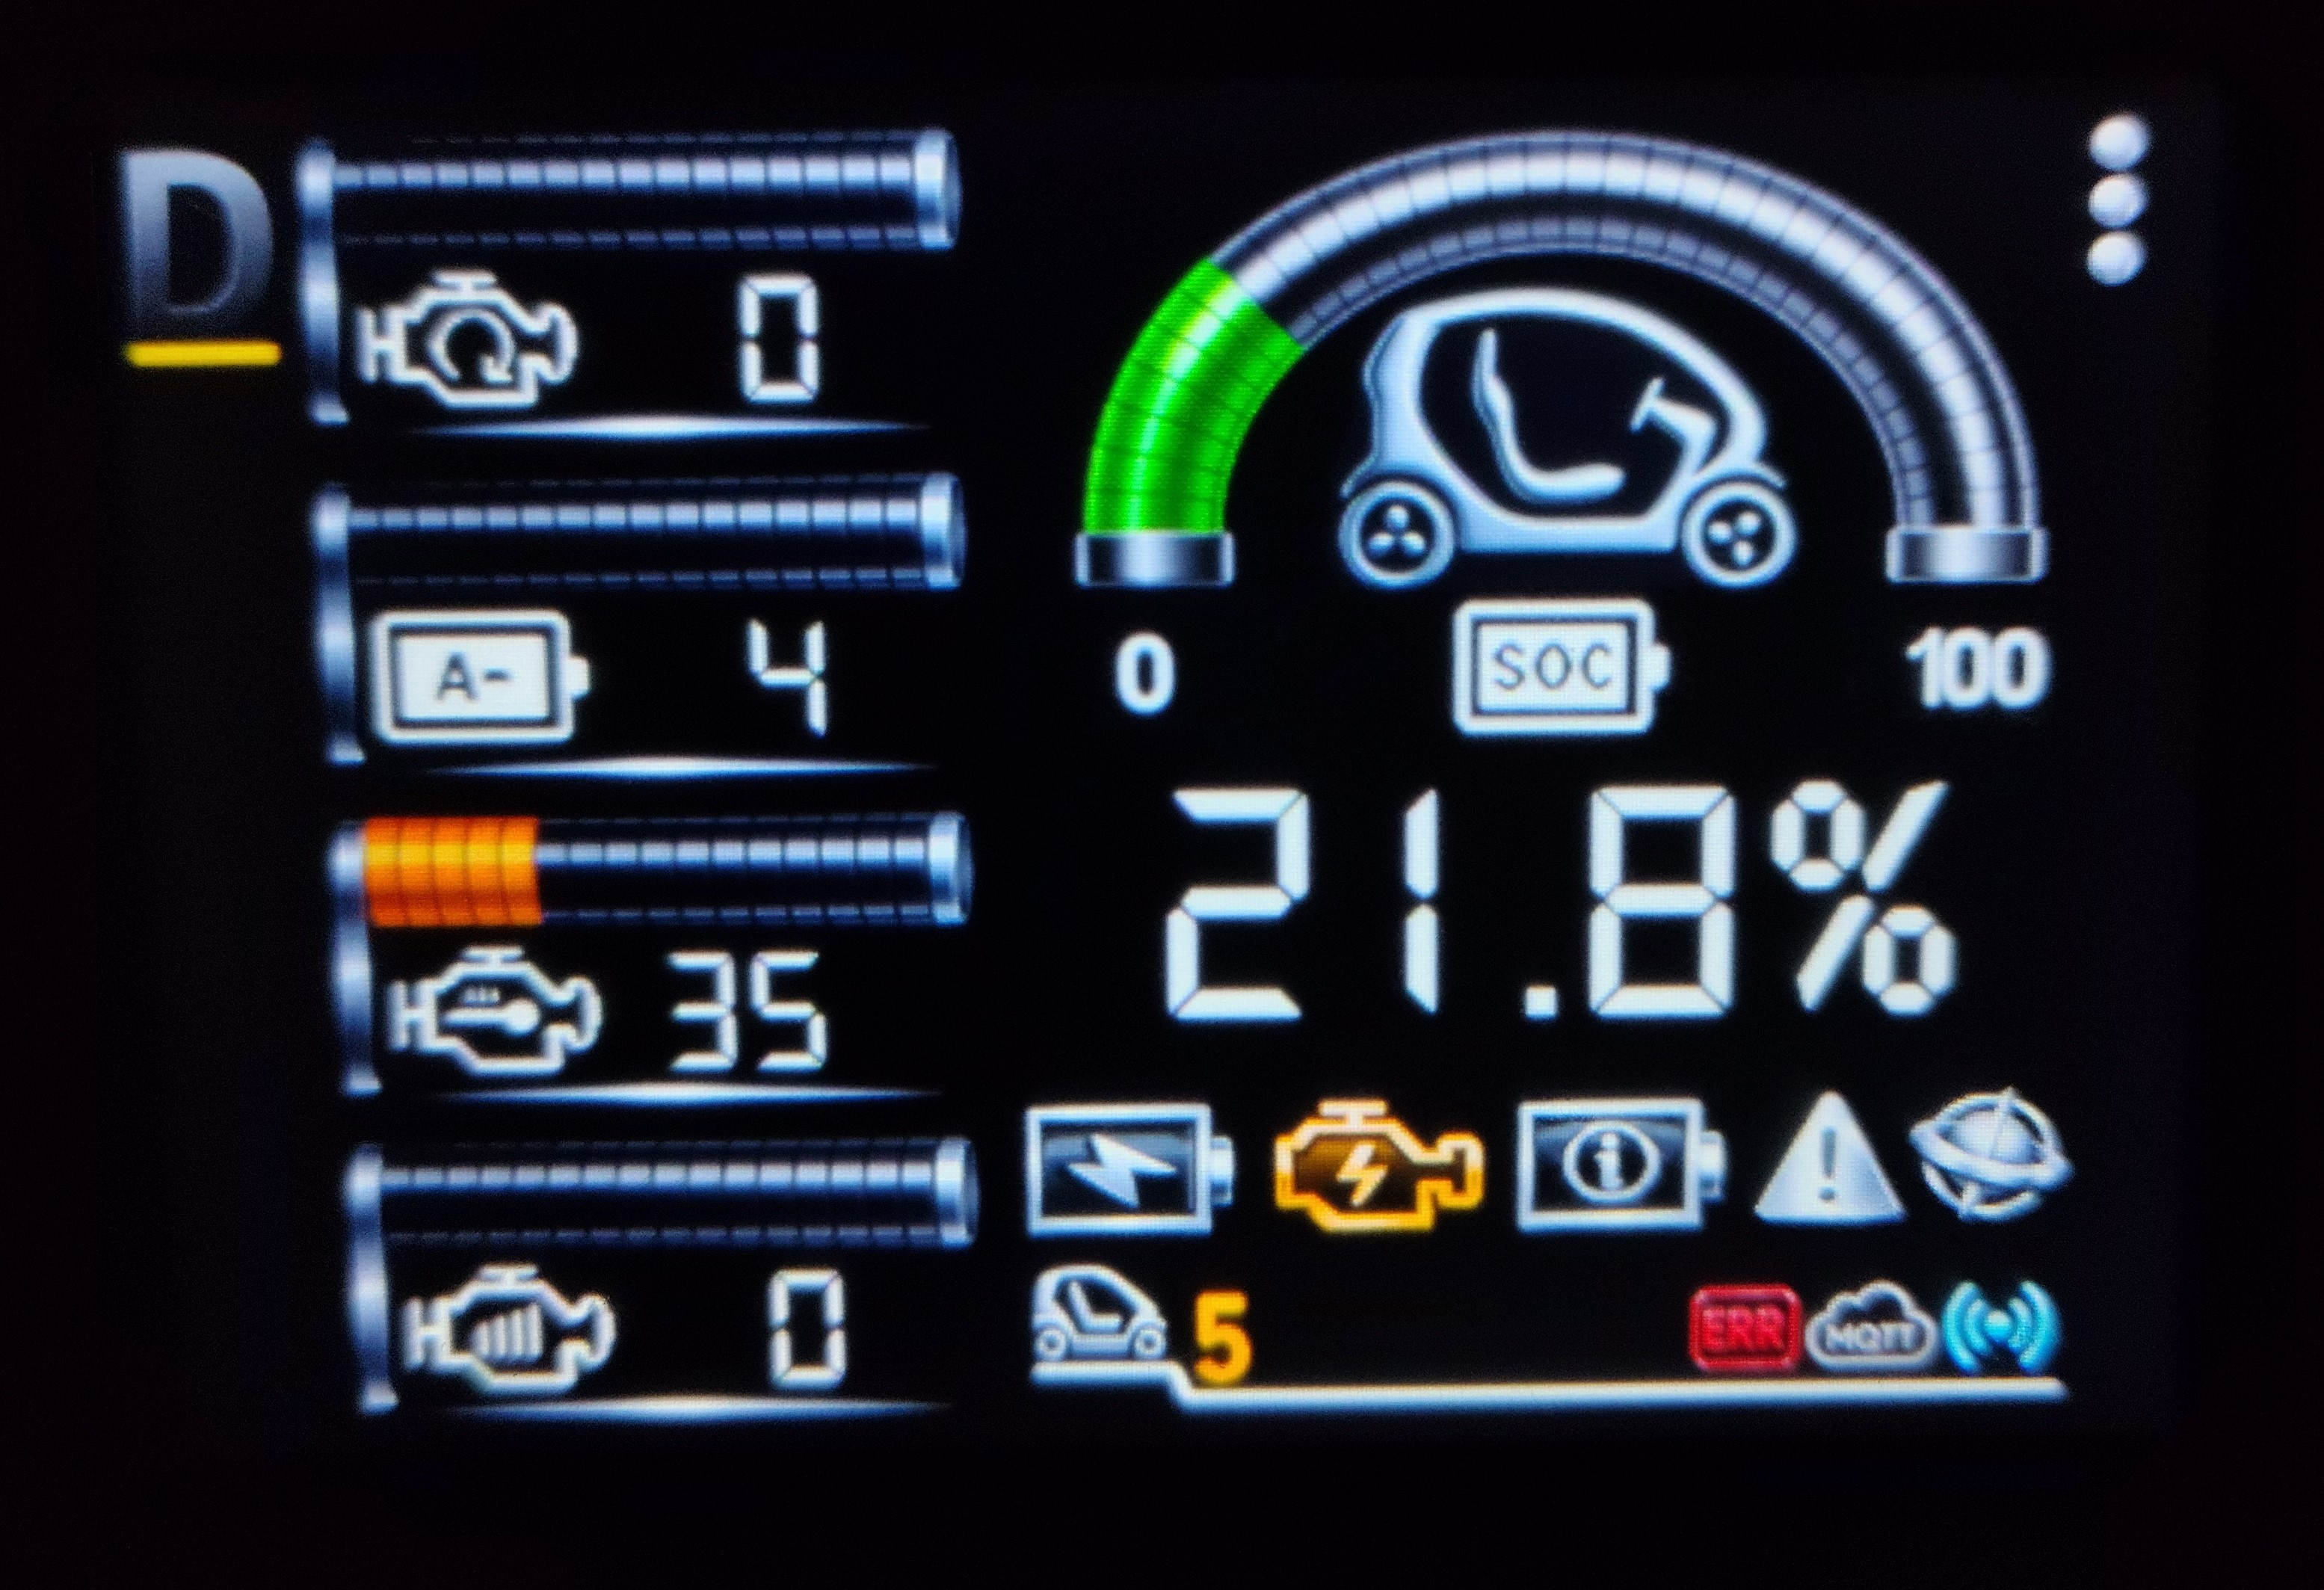
\includegraphics[width=0.8\textwidth]{figures/engine_page.jpg}
    \caption{Example of the shared layout (the motor page).}
\end{figure}

In the left side of the screen, as you can see in the photo, there is a list of four values,
grouped into a minimal grid. Each value is paired with its measure unit and a small
icon, which is unique for each data and all of them were listed in Section~\ref{sec:icon_list}. 
Above the value there is an orange progress bar which represents how big
(or small) is the value compared to its maximum (or minimum) value.\\

The right area of the screen is mainly occupied by the foreground data (or simply
selected data). It has a big Twizy icon surrounded by an arch shaped progress bar
which does the same function of the smaller one discussed before with the only
difference that it has 32 steps instead of 16 only. At the edges of the progress bar
there is the range or the multiplier of the value shown in the center of the page, which
is the one associated with the icon shown just above it.\\

In the bottom there is a list of icons, which are used to switch between the different pages of the ToM+. The icons are
the same for all pages, and they were all listed in Section~\ref{sec:page_icon_list}.
In the top left corner there is a small icon which shows the current gear of the vehicle.
If pressed, \textbf{it will take you back to the dashboard page}, we've just discussed.
In the top right corner there are three small dots, which if pressed will open the settings page.
Lastly, on the long white line at the bottom of the screen, there is the status bar with some icons we will discuss later.

\subsection{Changing the foreground data}

Changing the data shown in foreground is really easy and intuitive. You can do it just by 
tapping on the icon of the data you want to show in foreground and the values will swap.
In this way you can also rearrange the data in the left side of the screen,
which is really useful if you want to have a specific data in an arbitrary order.

\begin{figure}[H]
    \centering
    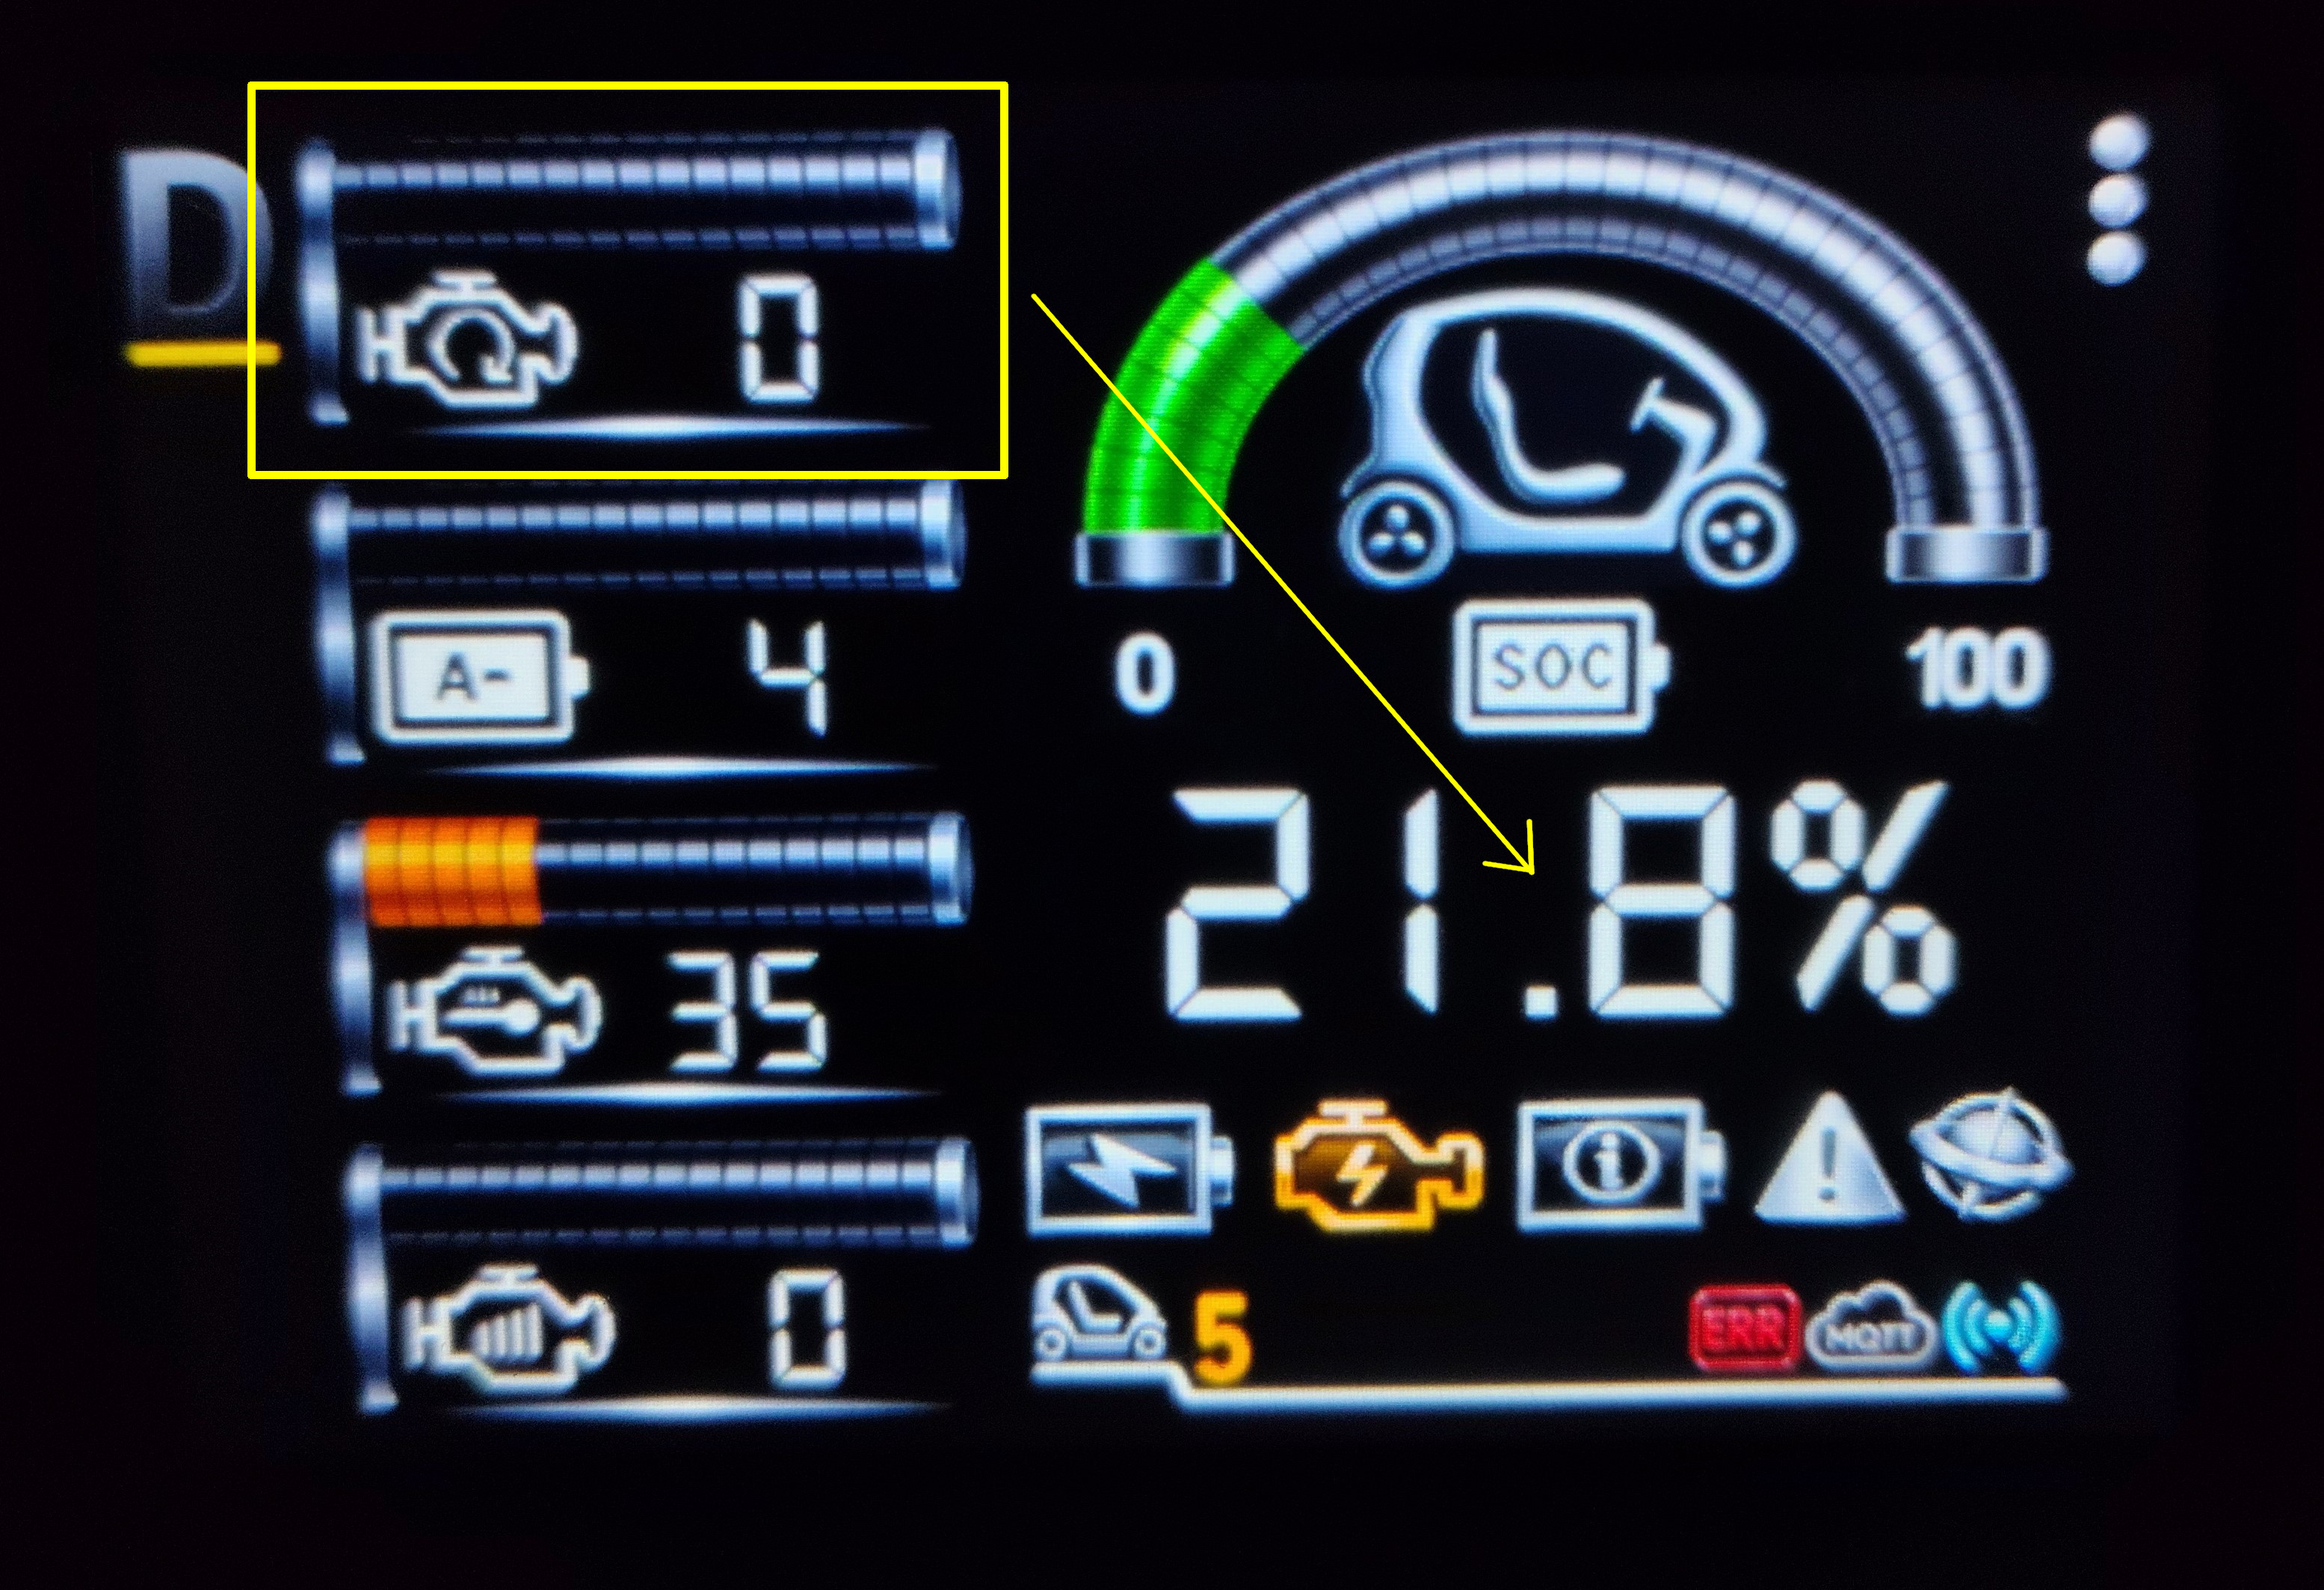
\includegraphics[width=0.7\textwidth]{figures/change_foreground.jpg}
    \caption{Example of changing the foreground data (in the motor page).}
\end{figure}

As an example, in the picture above, the user has tapped on the icon of the motor RPM, which is
currently shown in the left side of the screen. The two values have swapped and now the motor 
RPM is shown in foreground, while the battery SOC is shown in the left grid.

\subsection{Changing the active page}

To change the active page, you can tap on the icon of the page you want to switch to, which is located in 
the bottom line of the screen. The icon will become orange and the new page will be displayed.
In the image the active page is the motor page.

\begin{figure}[H]
    \centering
    
\includegraphics[width=0.7\textwidth]{figures/changing_page.jpg}
    \caption{Example of changing the active page (in the motor page).}
\end{figure}

Each of these actions can be performed using the button on the right wiper stalk,
which is really useful when driving, since you can keep your eyes on the road and
your hands on the steering wheel. The button can be used to cycle between the different pages,
to change the foreground data and more. It will be described in detail in Section~\ref{sec:web_wiper_stalk}.

\subsection{The status icon bar}
\label{sec:status_icon_bar}

Below the buttons to change page discussed in the previous paragraph, there is a long
white line that will show you the network connection status and when alarms or errors
trigger as well. At the beginning of the line, as you can see in the picture, is located a
small twizy icon with a number: it's a button that will take you to the trip
page, that will be discussed later in Section~\ref{sec:trip_page}. Now let's see the status icon bar.

\begin{figure}[H]
    \centering
    
\includegraphics[width=0.7\textwidth]{figures/status_icon_bar.jpg}
    \caption{The status icon bar.}
\end{figure}

Starting from the right side of the image you will see a magnetic blue wave symbol
that stands for the \textbf{Wi-Fi} connection status. In fact if it's powered and fixed as it is
above it means ToM is connected to a Wi-Fi, which can be both a public network or
one from the list you set. When the icon is greyed out ToM is not connected to any
networks and will look for Wi-Fi networks again after a cooldown period of five minutes.
Or you can force a new scan as soon as possible by tapping on the icon.
Last but not least if the icon is blinking ToM has performed a Wi-Fi scan
finding one or more networks and is trying to connect to one of them.\\

The next icon is a purple cloud with the \textbf{“MQTT”} text in it and, as you can guess,
stands for the \textbf{MQTT} connection status. The position of this icon is fixed and can't be
changed, as it is for Wi-Fi one. Another similarity with the previous icon is that can
be either fixed or greyed out with the same color code as before.\\

Then we have the error icon, which is a red rectangle with the \textbf{“ERR”} text in it.
It will be displayed when an error is present or hidden when there are no errors.\\

Finally we have alarm icons, represented with colored stars. Stars available are the one
shown in the picture, you can select which one to use for each alarm in the web server Alarm triggers page.
There you can choose whether to make them blink or not.

\begin{figure}[H]
    \centering
    
\includegraphics[width=0.7\textwidth]{figures/alarm_icons.png}
    \caption{The alarm icons.}
    \label{fig:alarm_icons}
\end{figure}

\subsection{Pop-ups}

On these pages, pop-ups will appear, depending on your configurations set on the
web server “Alarm triggers” page. There are two main types of pop-ups: the
first one that won't disappear until you notice and press it (this type will block
the whole system, pausing the values in the left grid and the foreground value as well). 
Otherwise, if you don't want to be bothered while driving you can use the second pop-up type, which
was specifically designed to automatically disappear after 10 seconds. \\

Here you can see an example of the simplest type of pop-up where the circled
warning icon will keep blinking. As you can see it's composed by a yellow box with
a dotted outline which contains the icon of the value and the value itself that triggered
the alarm previously set on the web server page (motor temperature = 35\textdegree~C).

\begin{figure}[H]
    \centering
    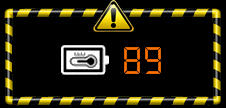
\includegraphics[width=0.7\textwidth]{figures/pop-up.PNG}
    \caption{An example of a pop-up.}
\end{figure}


\section{The battery info page}

The battery info page will give you more detailed info about every single cell of the
battery. As you may know standard Twizy batteries have 14 cells and a shared temperature sensor for each couple of them.
In this page you are able to monitor each cell voltage and its temperature as well, and you can also have an
overview of the full battery voltage. In the image is shown how it usually looks like.

\begin{figure}[H]
    \centering
    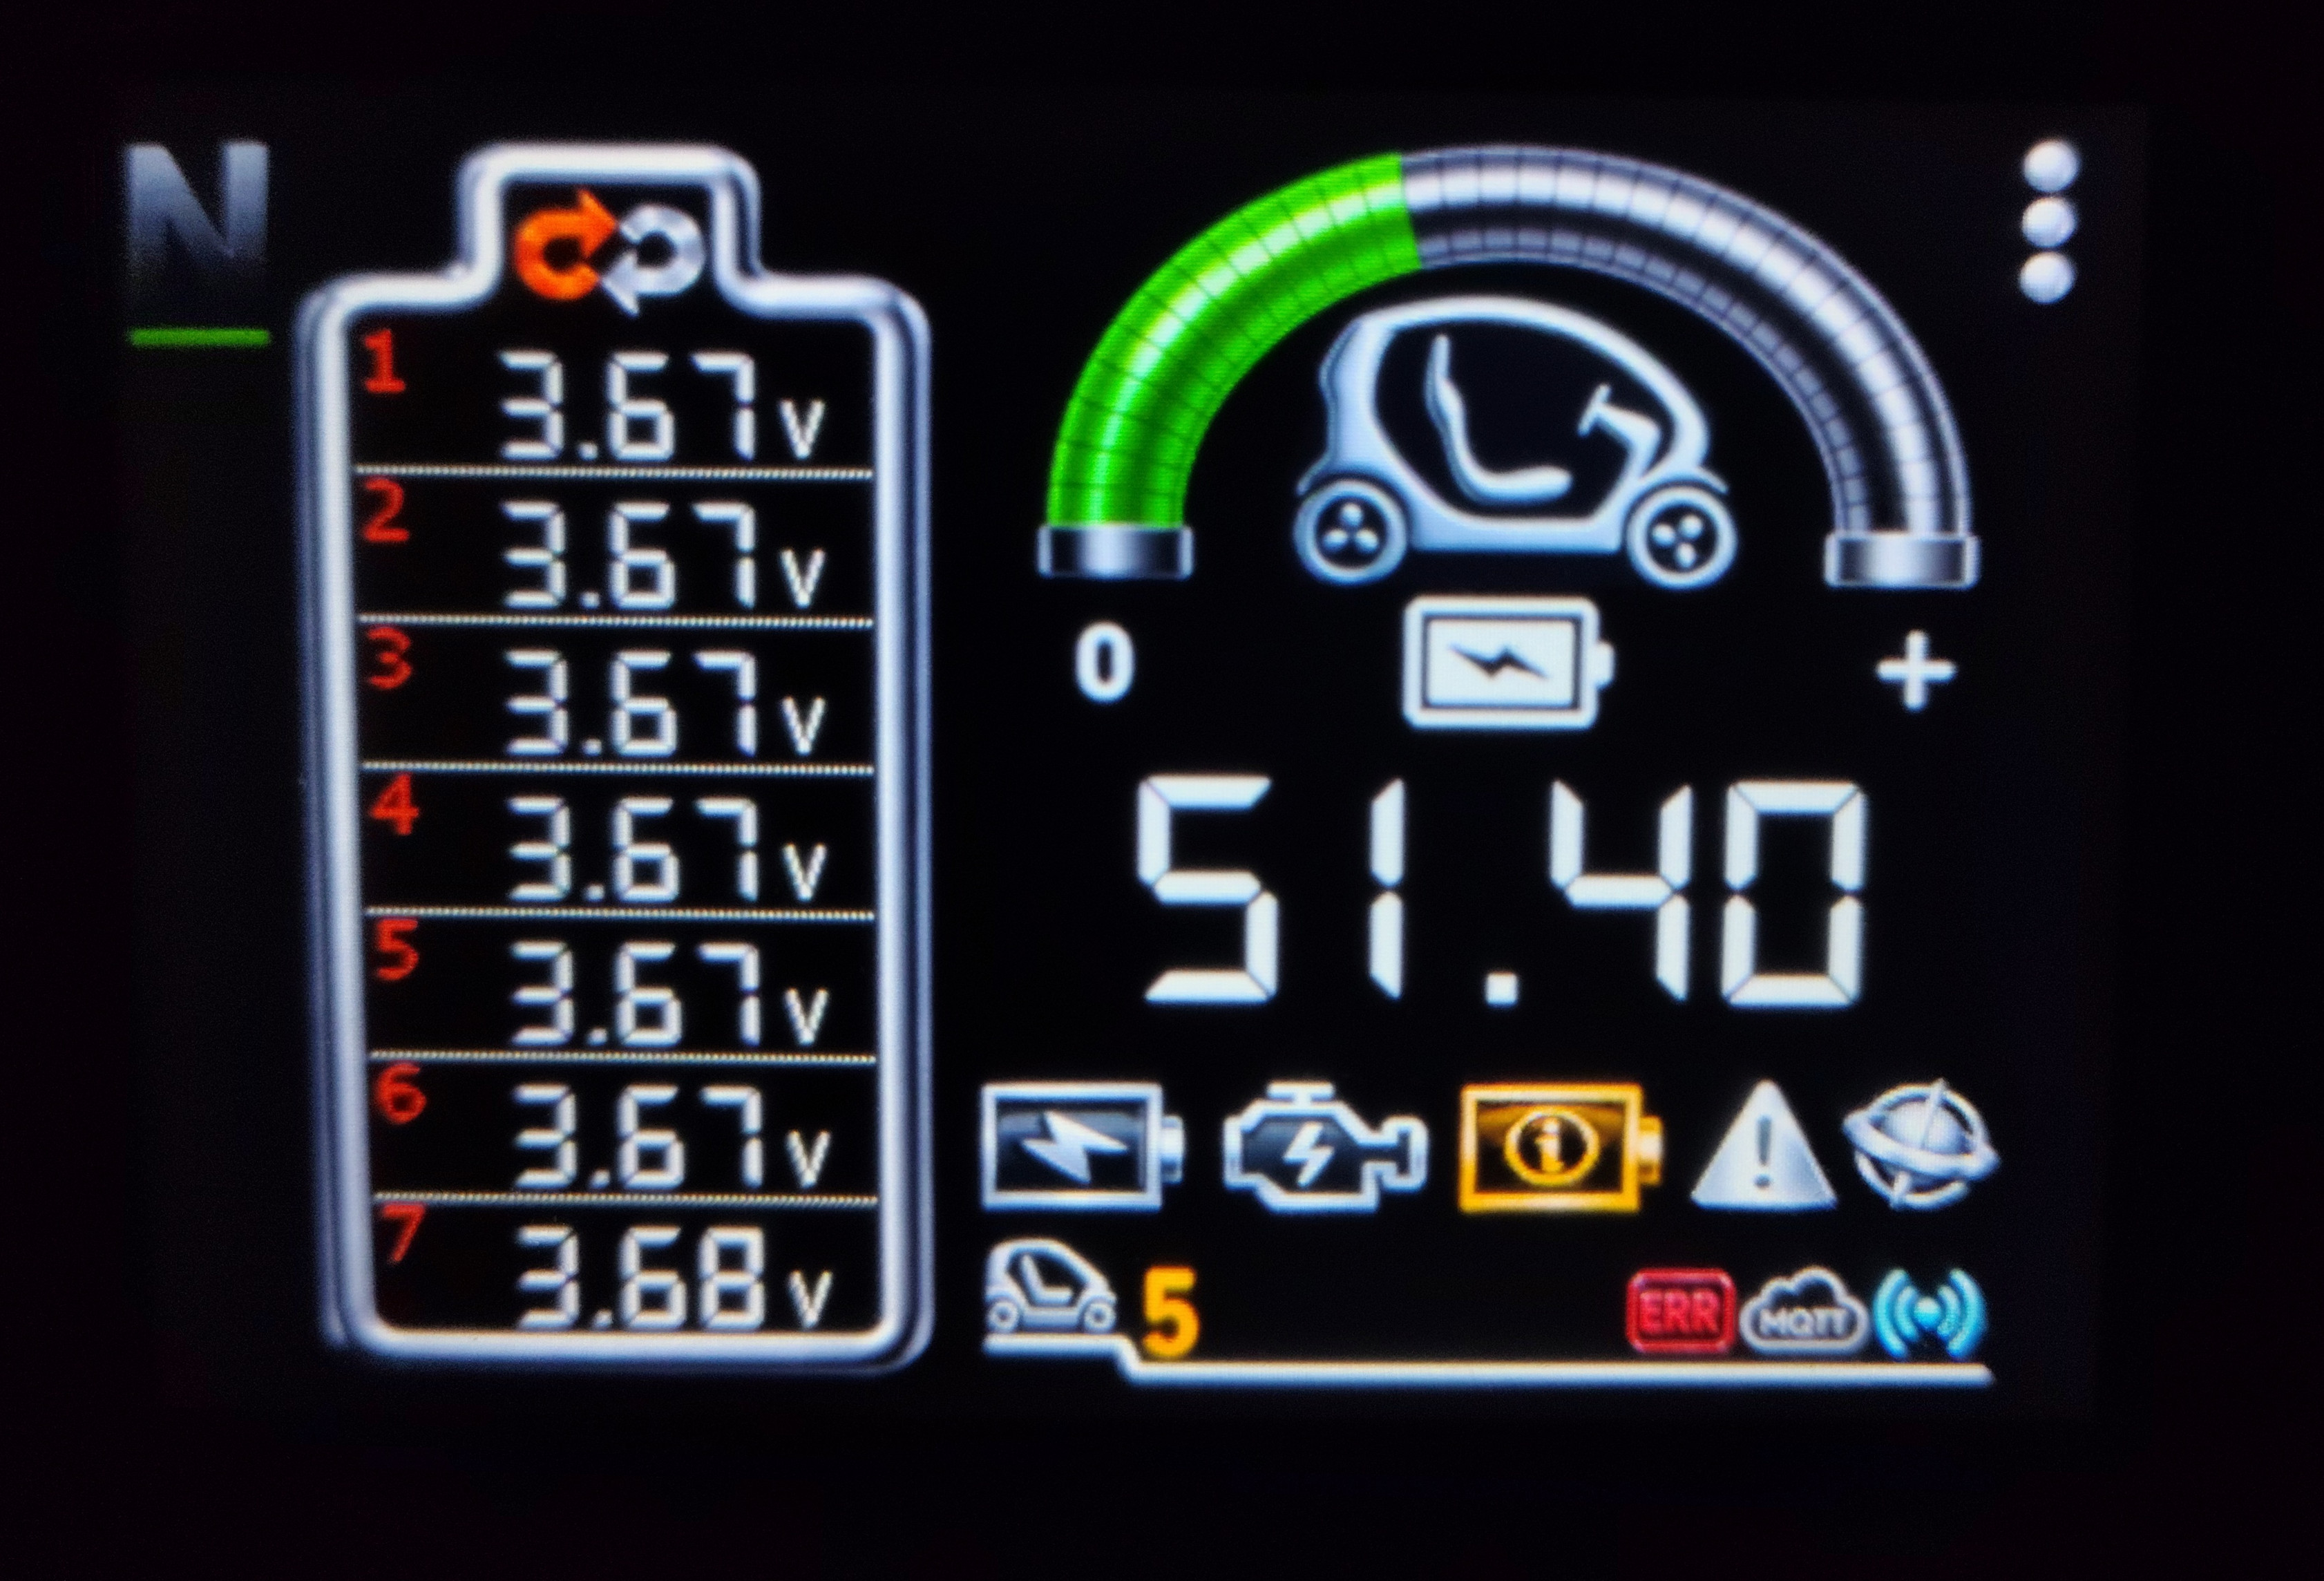
\includegraphics[width=0.8\textwidth]{figures/binfo_page.jpg}
    \caption{The battery info page.}
\end{figure}

\subsection{Checking voltage and temperature}

As shown in the image above in the left side of the page is located a battery shaped
white line which contains a small table with the first seven cells voltages. To see the
remaining cell voltages press the orange and white arrow symbol (the one circled
in the next photo) and the grid will show the next values.


If you press the same arrow button again the data shown will change again, becoming
the cells temperatures, expressed in Celsius. The foreground value would
change as well and as you may notice from the icon above it, showing the full
battery temperature, which is the same of each cell in this example. Refer to the image below to see the change.

\begin{figure}[ht]
    \centering

    \begin{subfigure}[t]{0.48\textwidth}
        \centering
        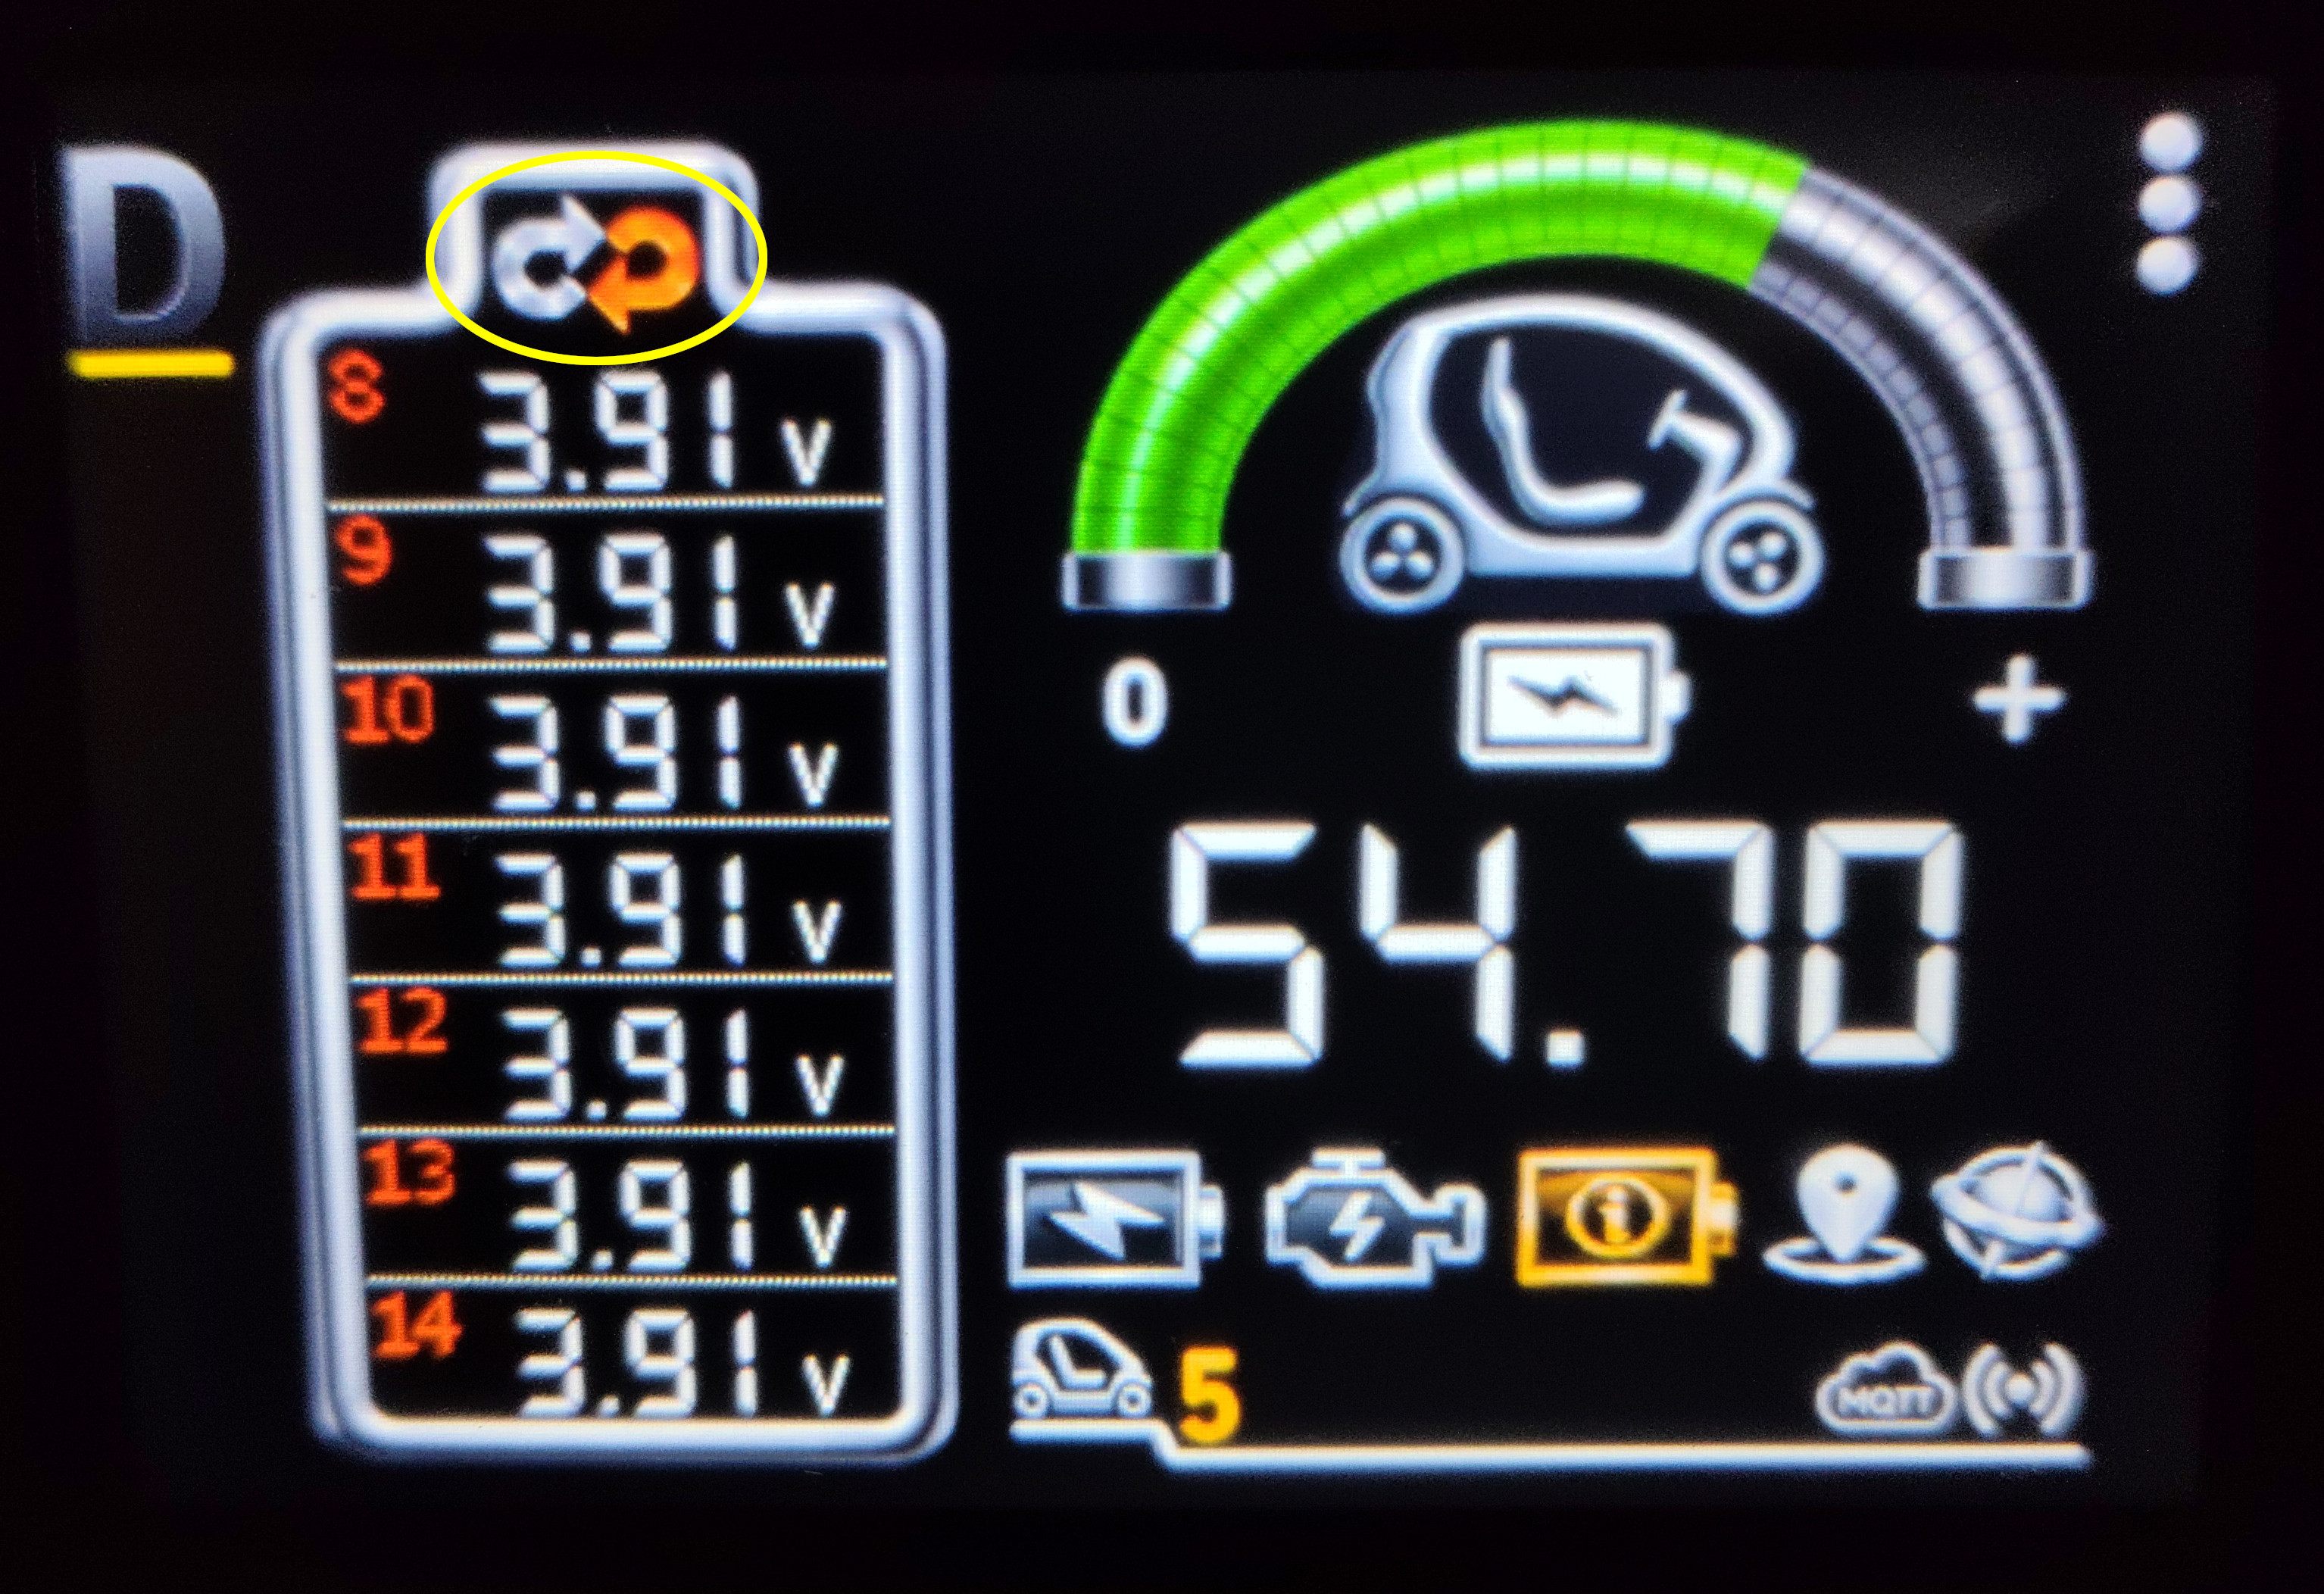
\includegraphics[width=\linewidth]{figures/binfo_page2.jpg}
        \caption{Remaining cell voltages.}
    \end{subfigure}
    \hfill
    \begin{subfigure}[t]{0.48\textwidth}
        \centering
        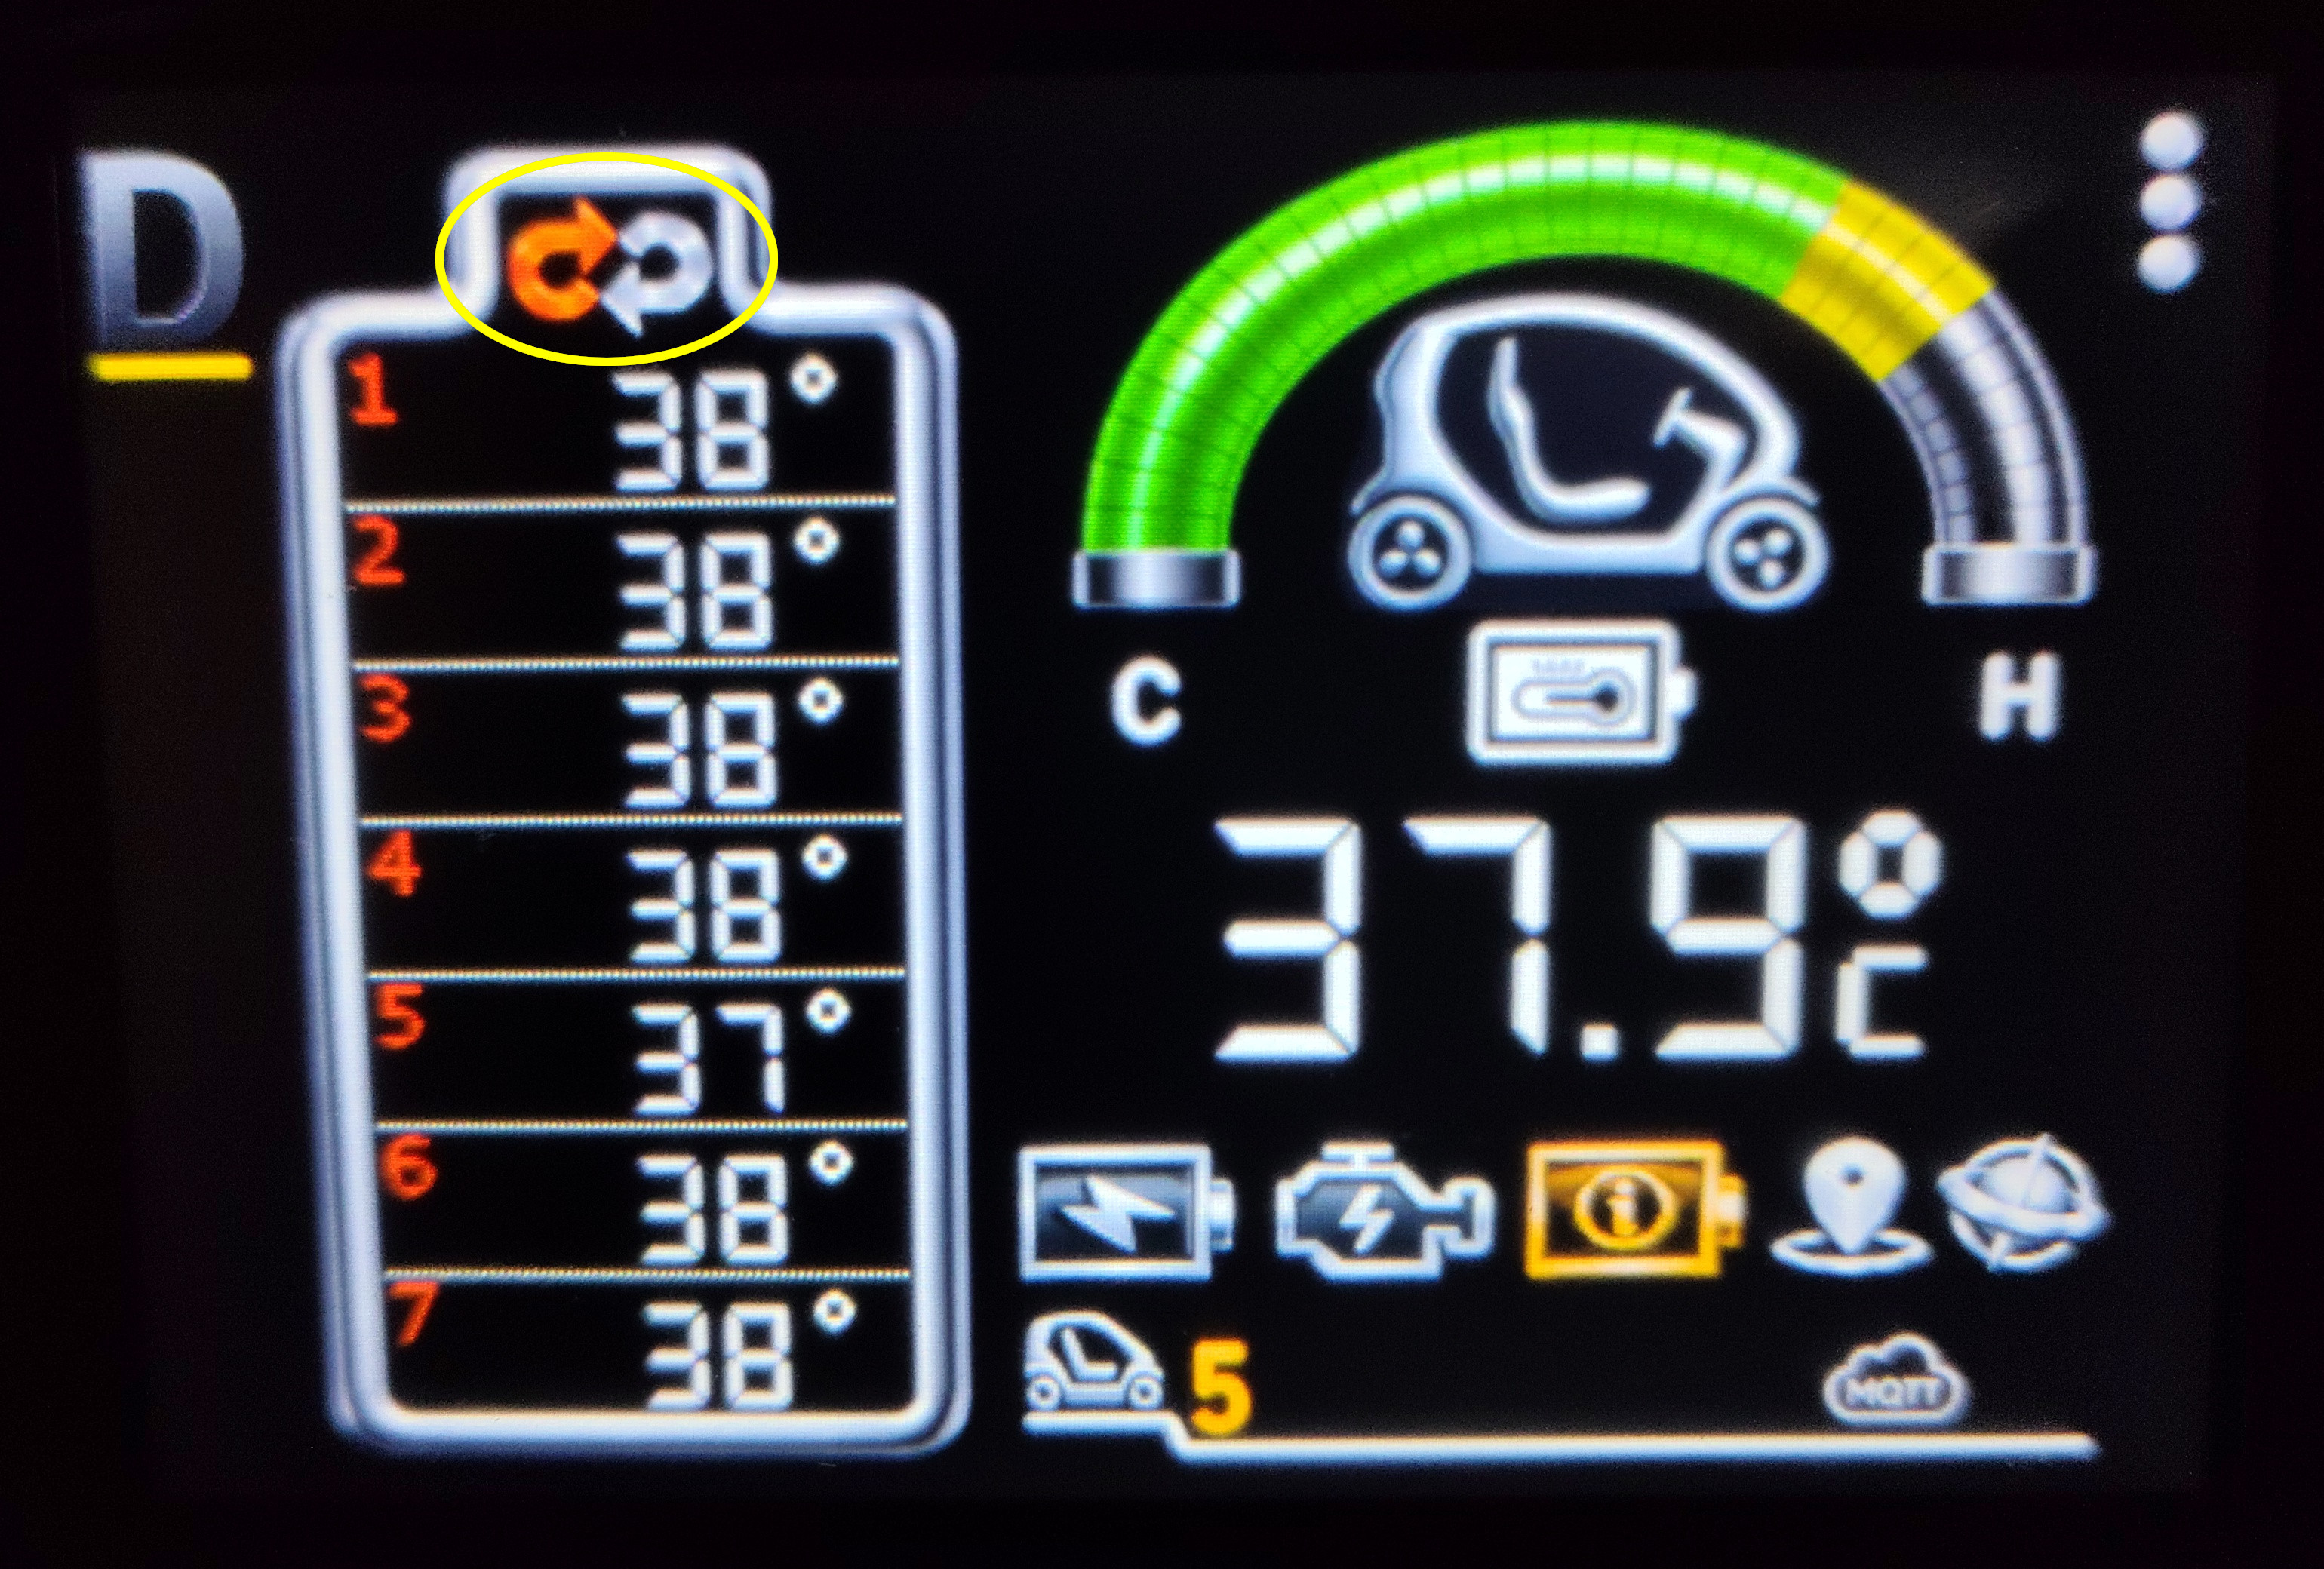
\includegraphics[width=\linewidth]{figures/binfo_page3.jpg}
        \caption{Cell temperatures.}
    \end{subfigure}
\end{figure}

\subsection{The condensed battery info page}
\label{sec:condensed_binfo}

Pressing the same button again will take you to a special page which contains all the
data we discussed in the previous paragraph at once.

\begin{figure}[H]
    \centering
    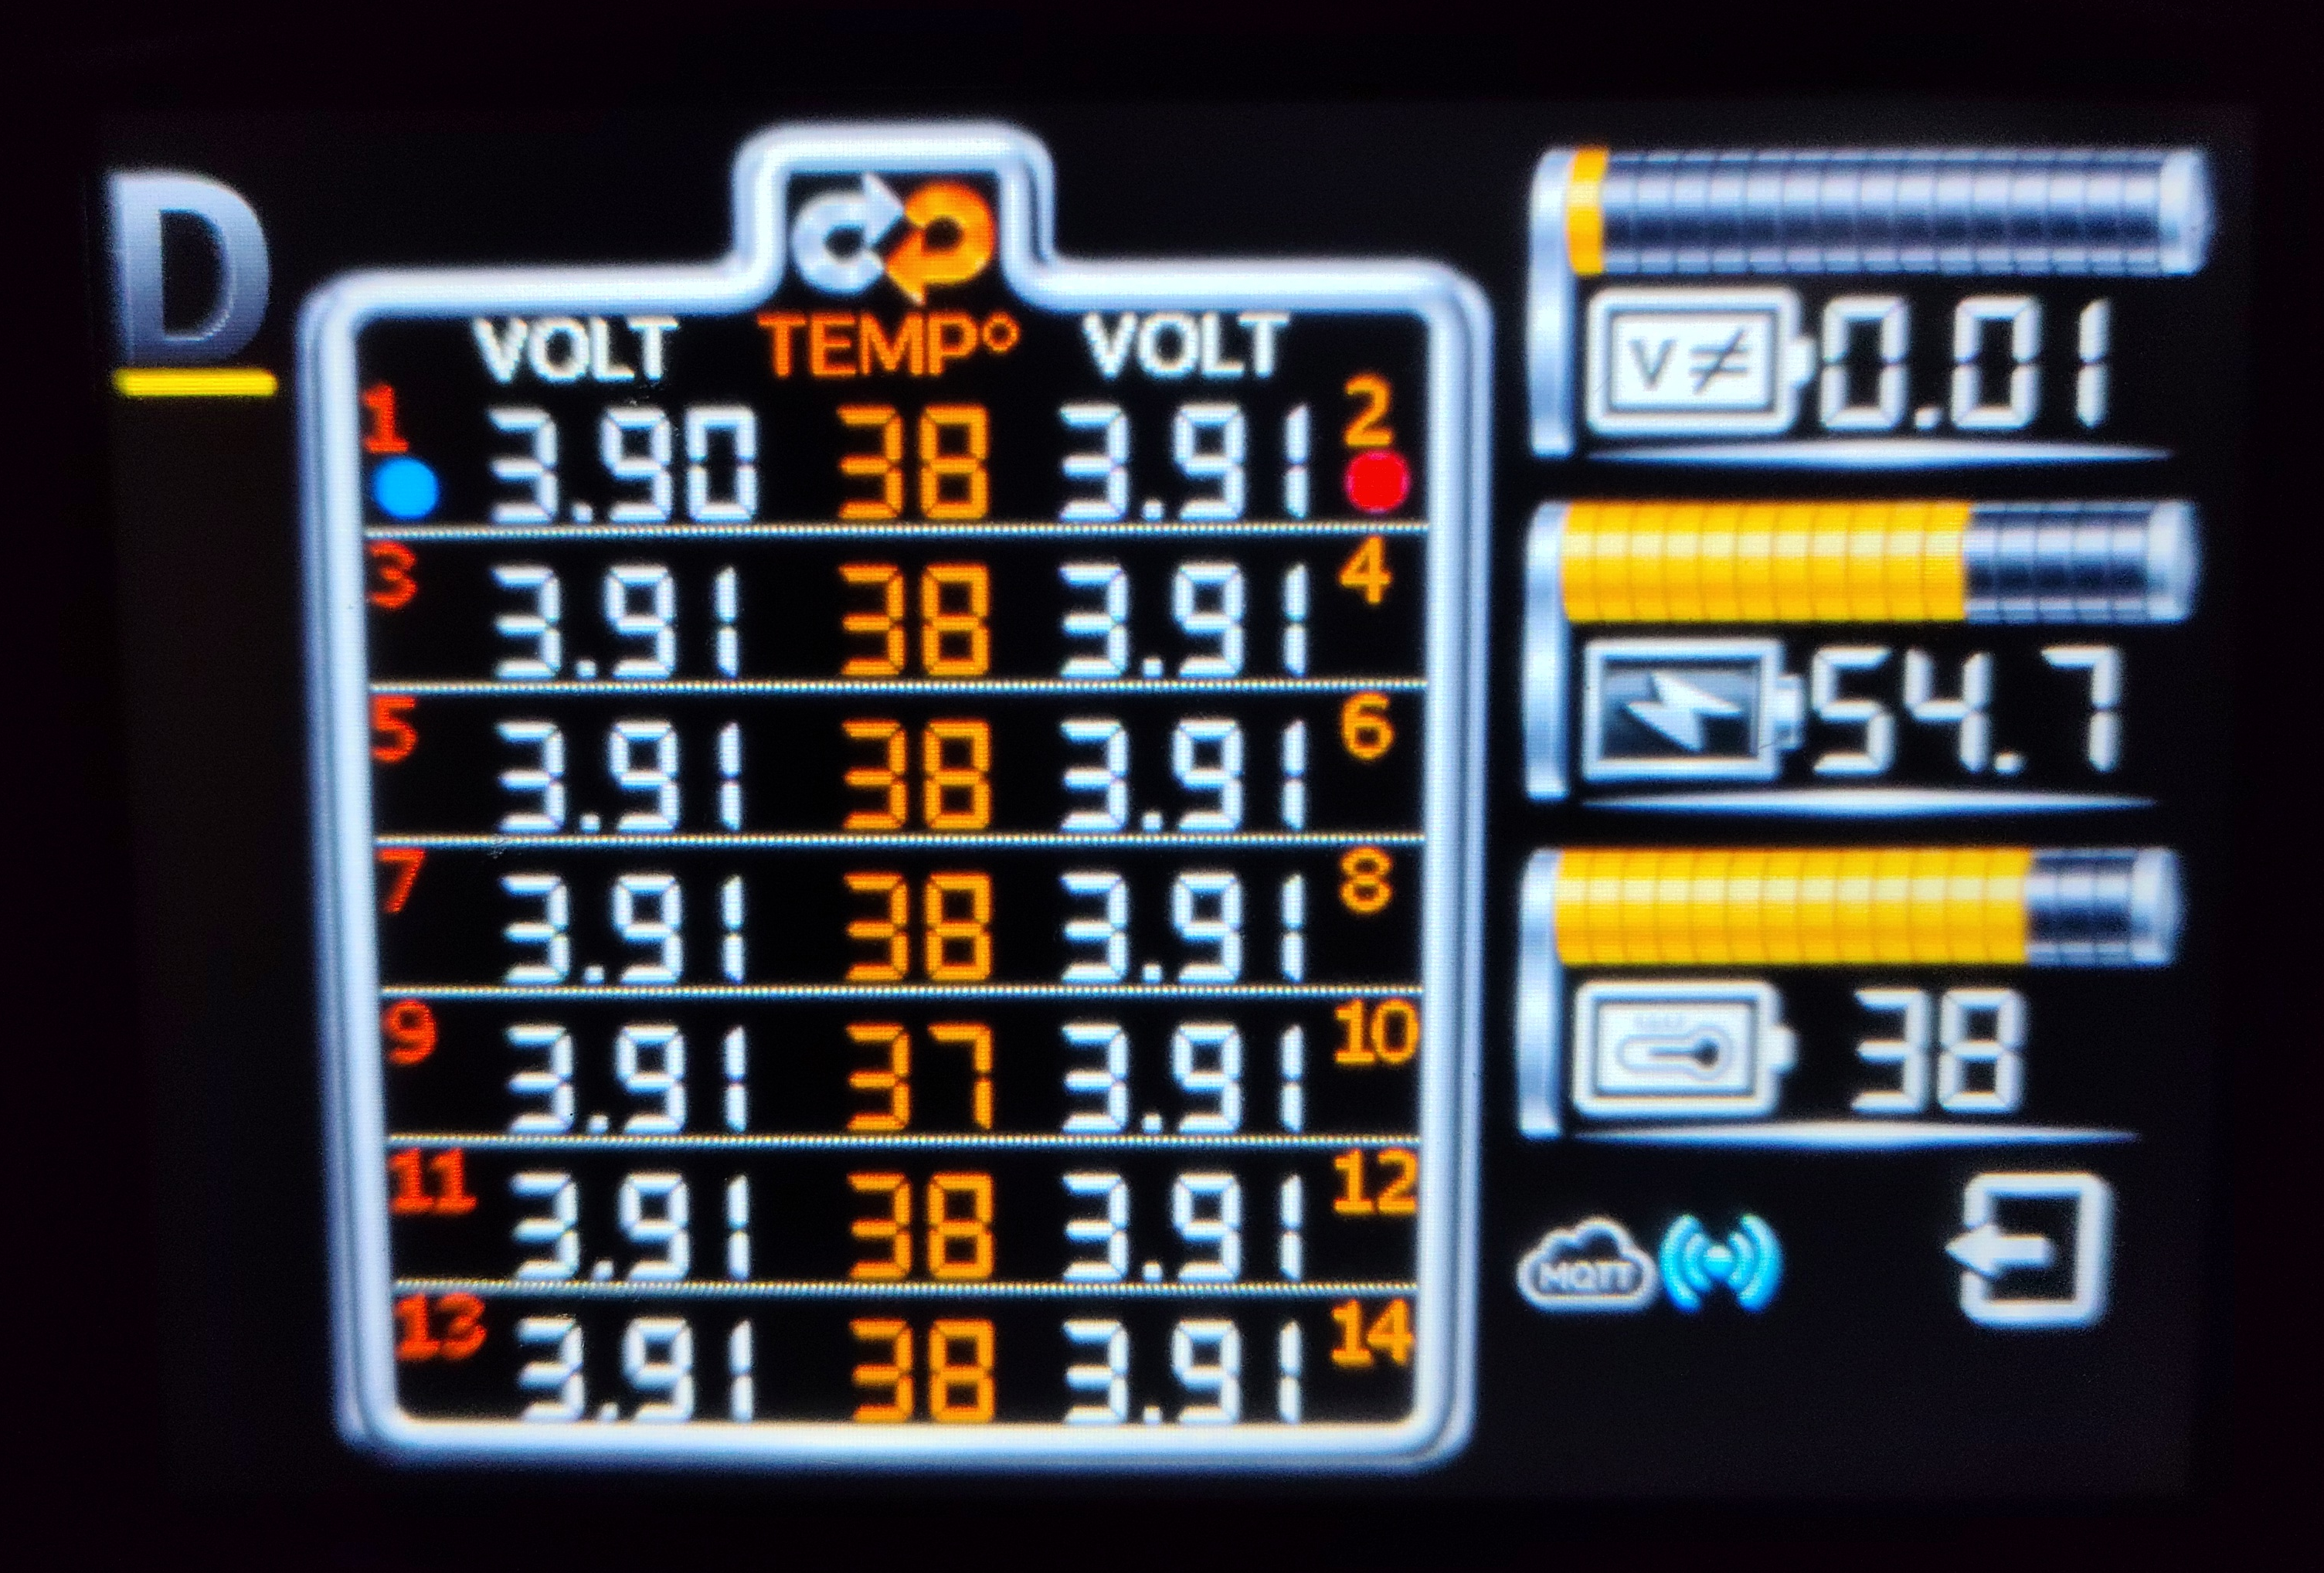
\includegraphics[width=0.8\textwidth]{figures/binfo_page_condensed.png}
    \caption{The condensed battery info page.}
\end{figure}

In the photo above you will see that the screen is divided in two parts. The first one is
the same battery shaped white line but a little bigger, in order to contain all voltage
and temperature values. The temperature is located between the two cells which share
that temperature sensor. In the right side of the page you can see the value that were
previously shown in foreground, i.e.~the full battery voltage and the full battery
temperature. There is also the SOC value in the first position because it's always
useful.\\

In this page there wasn't enough space to put the buttons to change page, because it's
more important to have those status icon we discussed before. If you need to change page you can press the exit
button in the bottom right corner and then you will be taken to a page that has the controls to change the active page.\\

An important note of the last update is the difference between the cell with the 
minimum and maximum voltage, respectively represented by a blue and red dot. 
This value is really important because it can tell you
if the battery is healthy or not. If the difference is too high, it means that 
the battery is unbalanced and it could be a sign of a problem. ToM+ will 
show you this value in the condensed battery info page, and you can also set 
an alarm trigger in the web server to be notified when the difference is too high.\\

You can decide in the settings whether this condensed battery page is shown as the
default page when you press the battery info button or not. The process is shown in
Section~\ref{sec:settings_page}. If you select the option to have all the four page we saw in this
paragraph, then you can also press the arrow button while on the condensed page to
cycle back to the other battery pages info.

\section{The alarm log page}
\label{sec:alarm_log}

In this page you will be able to see all alarm triggers, if you missed one or if you put
them silent not to be disturbed while driving. Let's see how it looks like.

\begin{figure}[H]
    \centering
    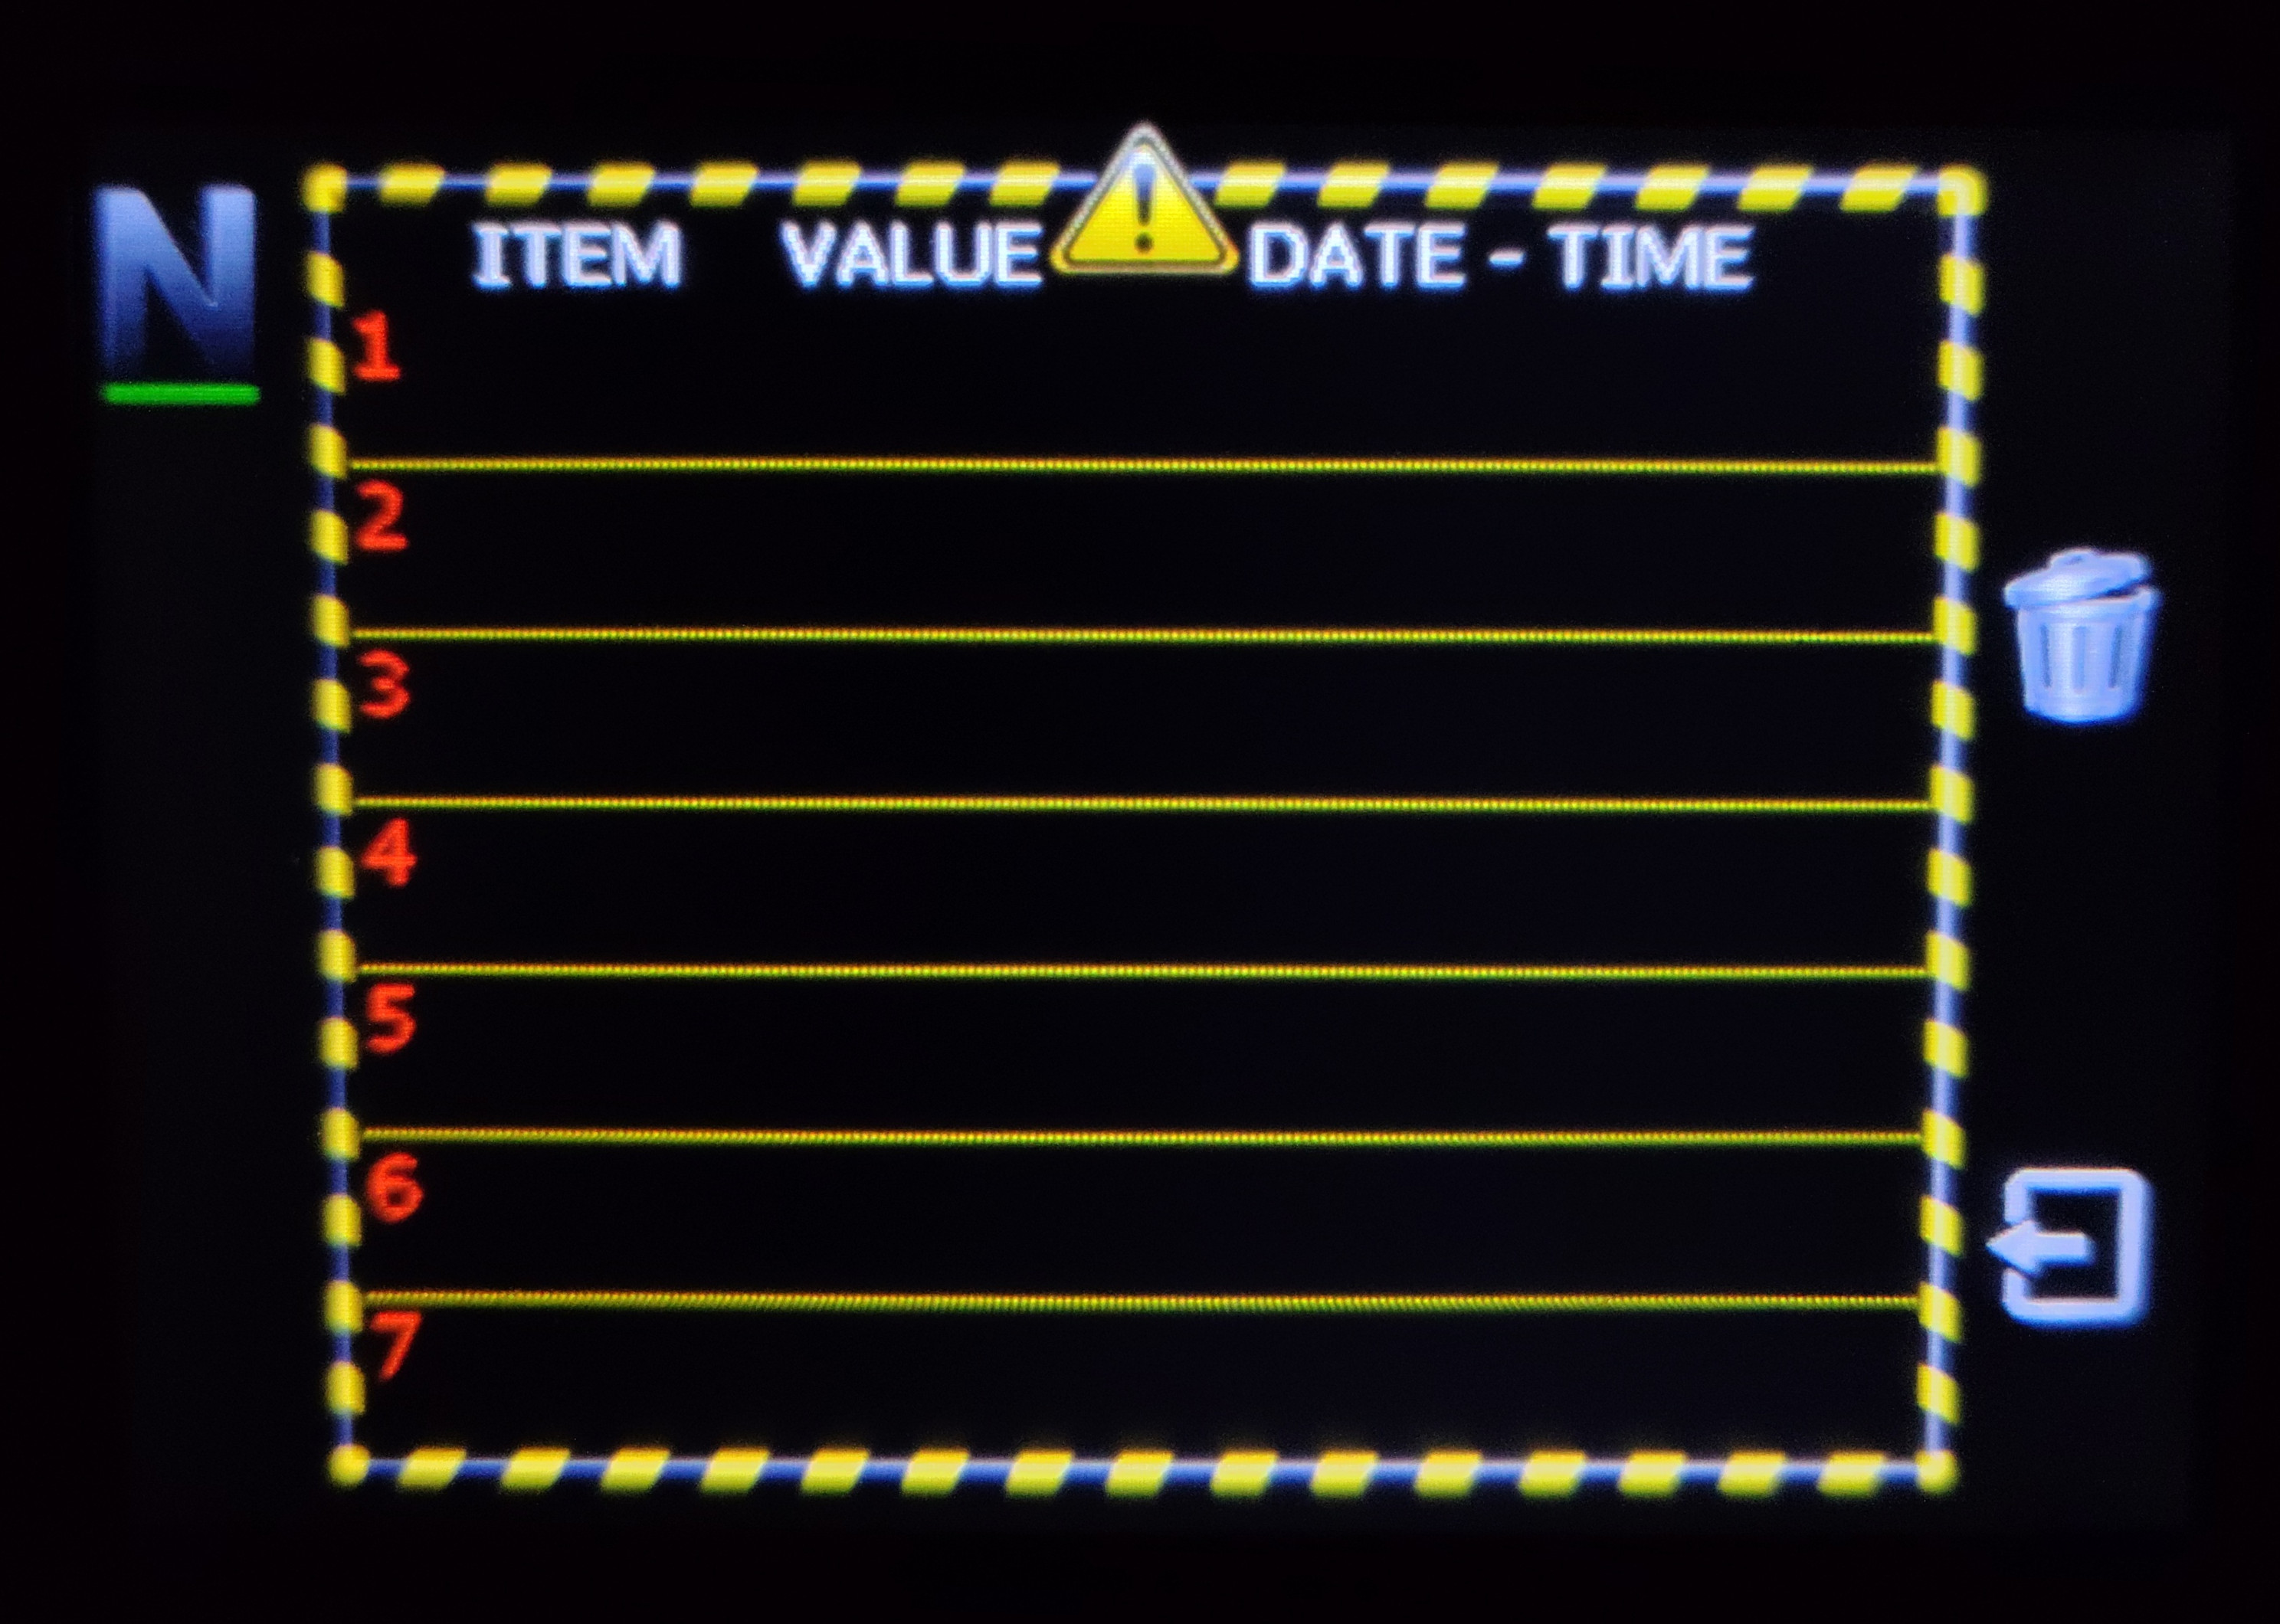
\includegraphics[width=0.8\textwidth]{figures/alarm_page.jpg}
    \caption{The 3D alarm log page.}
\end{figure}

The image show a small table which contains the item that caused the alarm to trigger
paired with its icon and its value. Then I added a date and time as well (available if
connected to a network the first time) to know when that record was added to the list.\\

In the next images (with the old design), most records are related to the battery SOC, specifically when it goes
below the 30\%. You will discover how to set your own alarm on the web server in Section~\ref{sec:web_alarm_triggers}.

\begin{figure}[H]
    \centering
    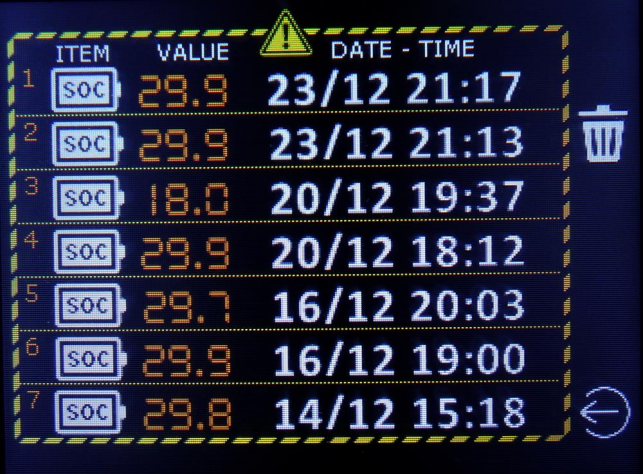
\includegraphics[width=0.7\textwidth]{figures/alarm_log_old1.png}
    \caption{The 3D alarm log page.}
\end{figure}

\subsection{Checking older alarm triggers}

If you need to see older alarm triggers, which doesn't appear in the list of the first
seven ones, then you can press the yellow warning icon at the top of the table, and
this will change the values shown with the older ones. You can do this action twice,
because ToM is able store up to 21 alarm triggers and forgets older ones.

\begin{figure}[H]
    \centering
    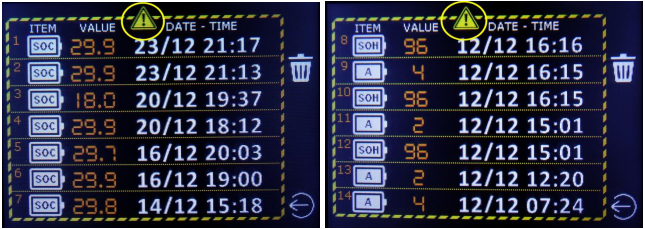
\includegraphics[width=1\textwidth]{figures/alarm_log_old2.png}
    \caption{Changing the shown triggers.}
\end{figure}

As you can see in these two photos of the alarm log page, when I pressed the circled
yellow warning button the data shown changed with some of the older ones as you
may notice comparing the dates. The item counter on the left changed as well (8--14).

\subsection{Deleting an alarm trigger}
\label{sec:delete_log_record}

If you don't need one or more records anymore, you can choose to delete some of
them. Select one or more records to permanently remove by pressing their date or time 
(a small red check sign will appear next to the chosen records). 
Then press the trash can icon circled in yellow in
the second photo to delete the selected records. Those records
will disappear and will be replaced by the next records, causing a shift of the whole
list as you may notice in the second picture.

\begin{figure}[H]
    \centering
    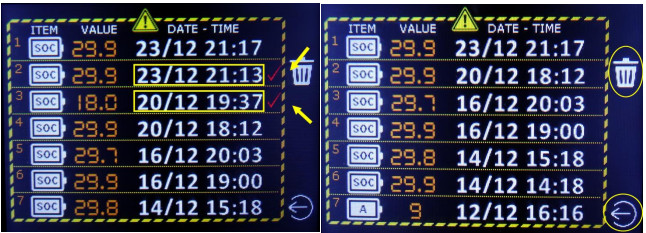
\includegraphics[width=1\textwidth]{figures/alarm_log_old3.jpg}
    \caption{Deleting selected alarm triggers.}
\end{figure}

In this page there aren't any status icon bar or buttons to change page, since it's quite
a settings page and doesn't need such controls. To exit, press the arrow button in the
bottom right corner and ToM will take you to the page you were before viewing the
alarm log page and from that you can change the active page again.

\section{The trip page}
\label{sec:trip_page}

This page is able to store the data about a trip \textit{(trip means the time from when you
start driving to when you power off your Twizy)} and then decide to store or discard
these values when you start driving again. You can store simultaneously up to five
trip data. The layout is the same as the main page, so the controls to change the order
of the values or the data in foreground was already discussed in Section~\ref{sec:main-layout}.
Next paragraphs are about how to reset a trip and how to change the current trip.

\begin{figure}[H]
    \centering
    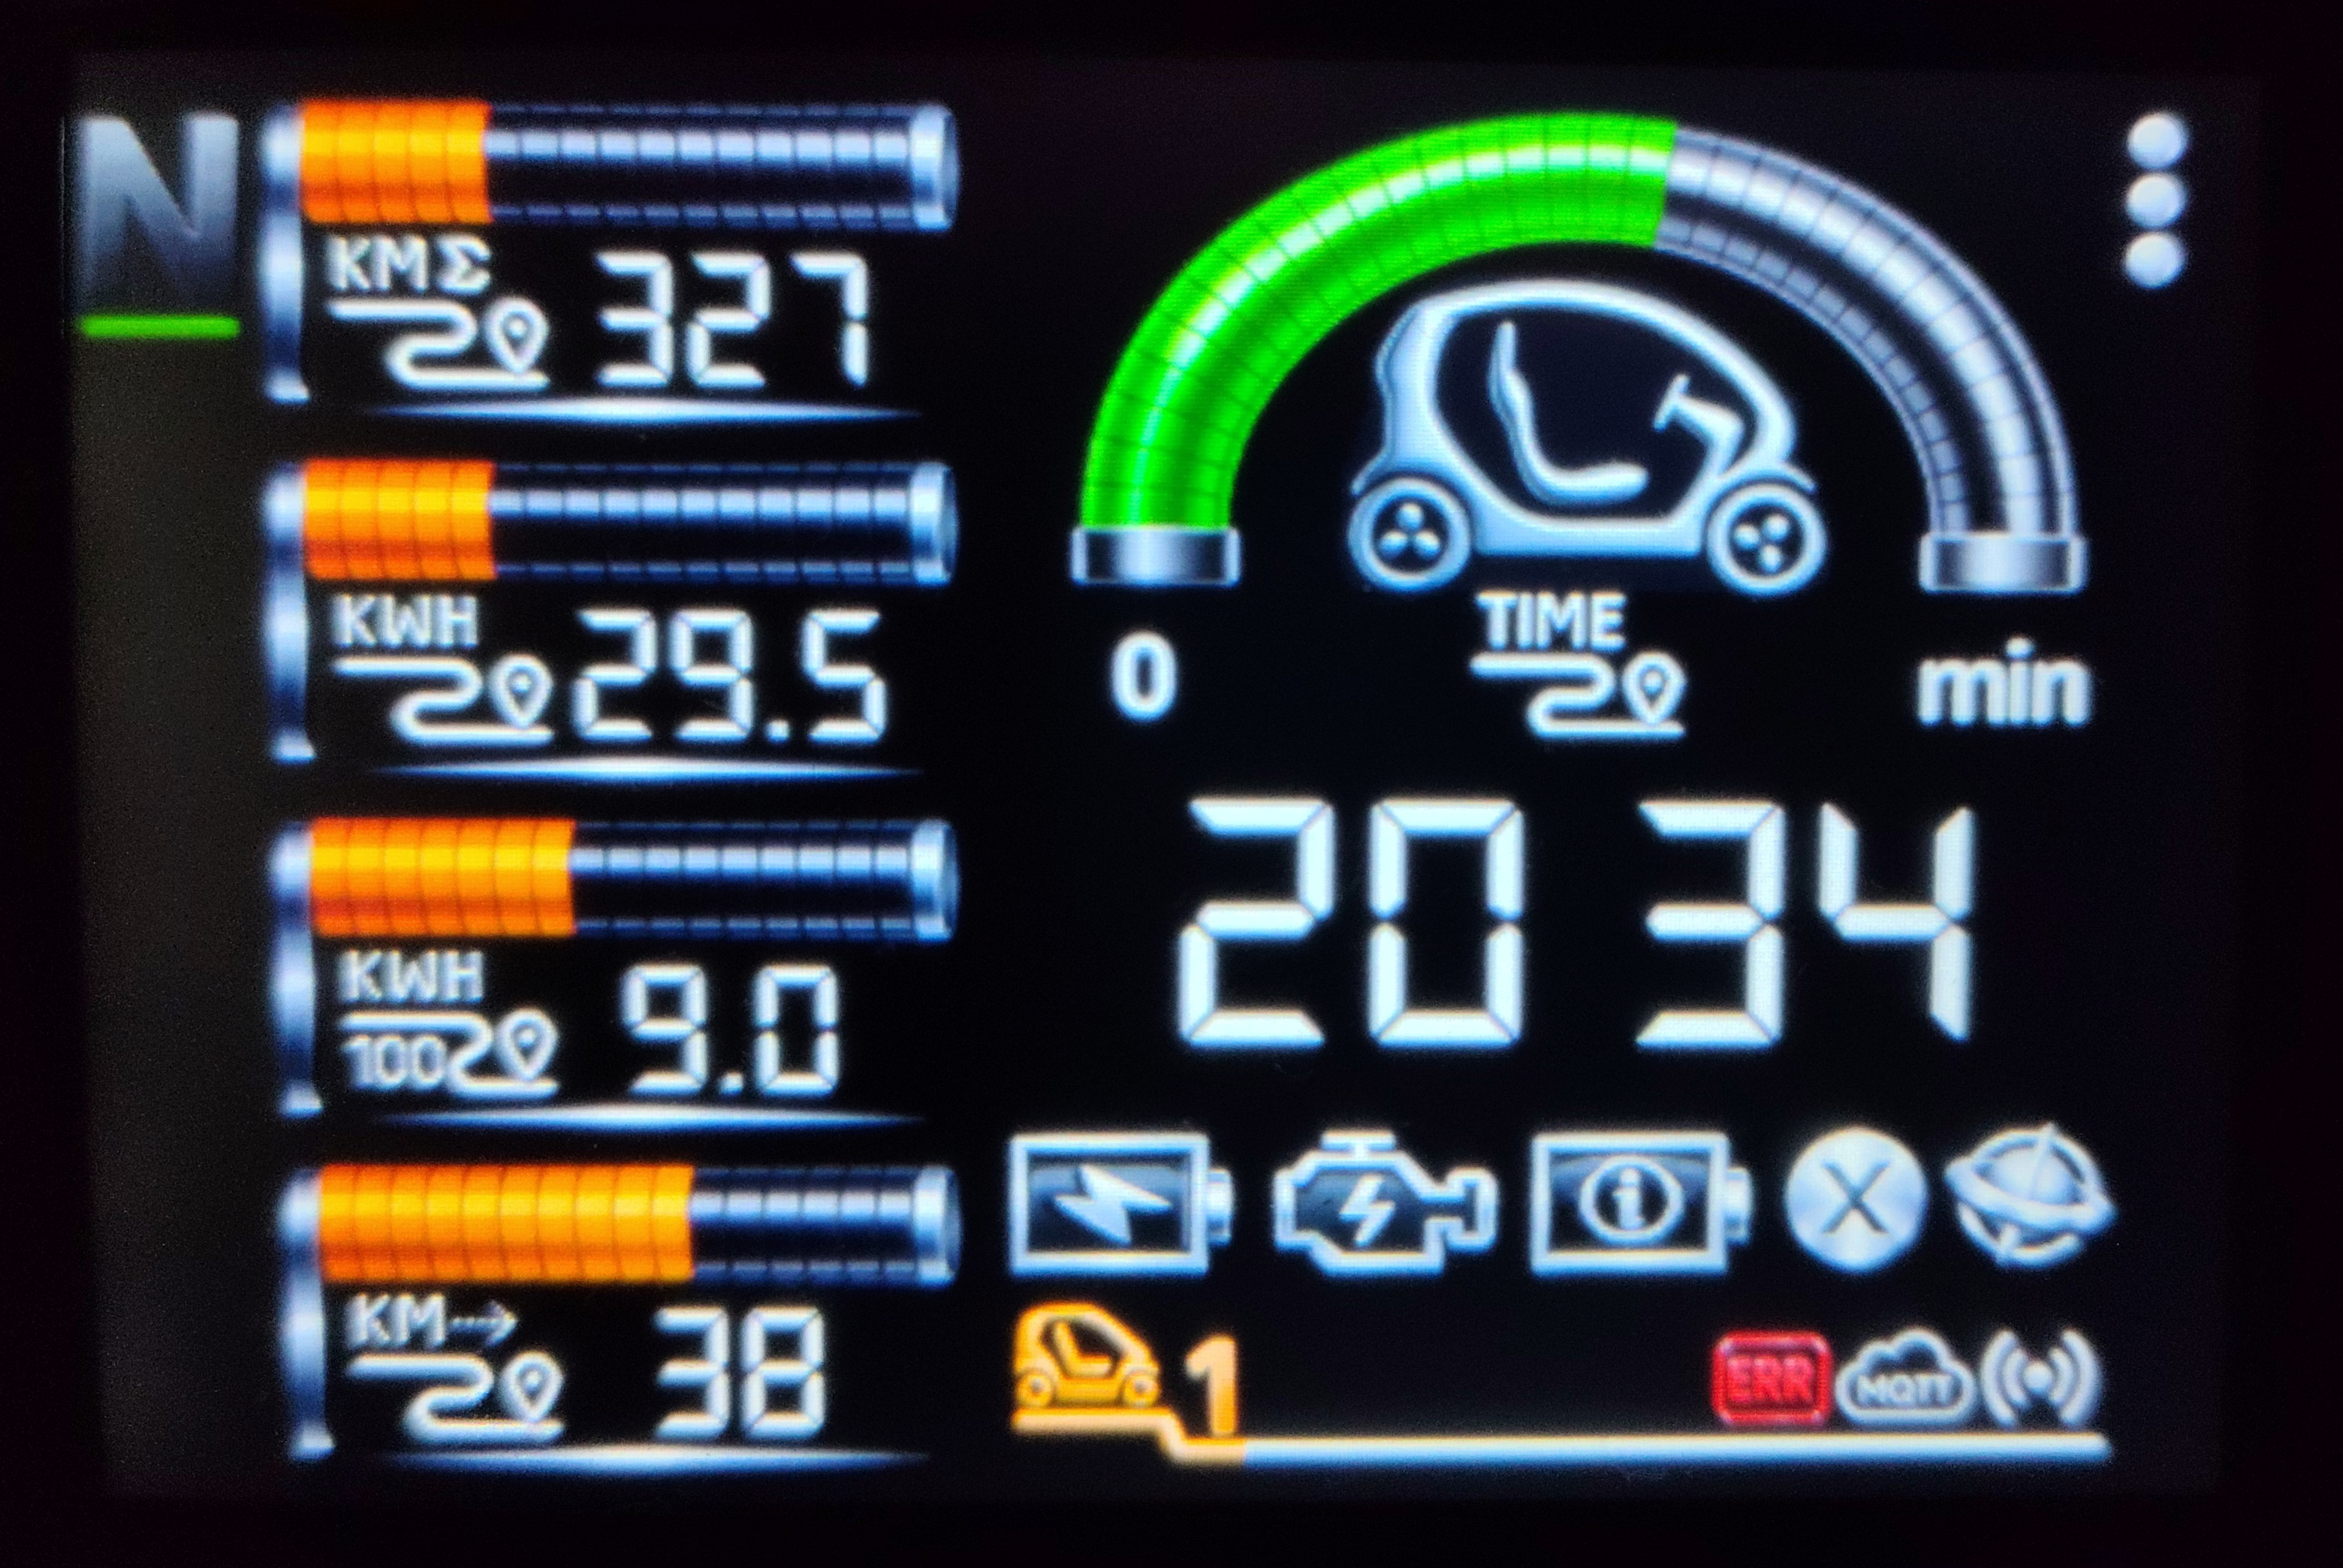
\includegraphics[width=0.8\textwidth]{figures/trip_page_full.jpg}
    \caption{The trip page.}
\end{figure}

\subsection{Changing the current trip}

If you want to start recording the data on a specific trip chosen from 1 to 5 you can
press the trip icon circled in yellow in the previous image. When you
first press it, you will be taken to the trip nr. 1 and pressing it again and again will
cycle through all the available trip, so that you can select the one you would like to
start or continue.\\

To see in what trip ToM is currently recording refer to the orange
number in the trip icon. Once you choose the desired trip you can also change the
active page if you want, without losing the selected trip, because ToM will keep
recording values even if the trip page is not focused.

\subsection{Disable trip recording}

In this example I'm currently on the motor page and I'm recording data on the fifth
trip page, as it's specified by the small orange number near the trip icon. If you want
to pause the trip recording, you can do that on ToM+ by \textbf{holding down for three seconds the trip button} while
another page is active (in this example the battery one).\\

\begin{figure}[ht]
    \centering

    \begin{subfigure}[t]{0.48\textwidth}
        \centering
        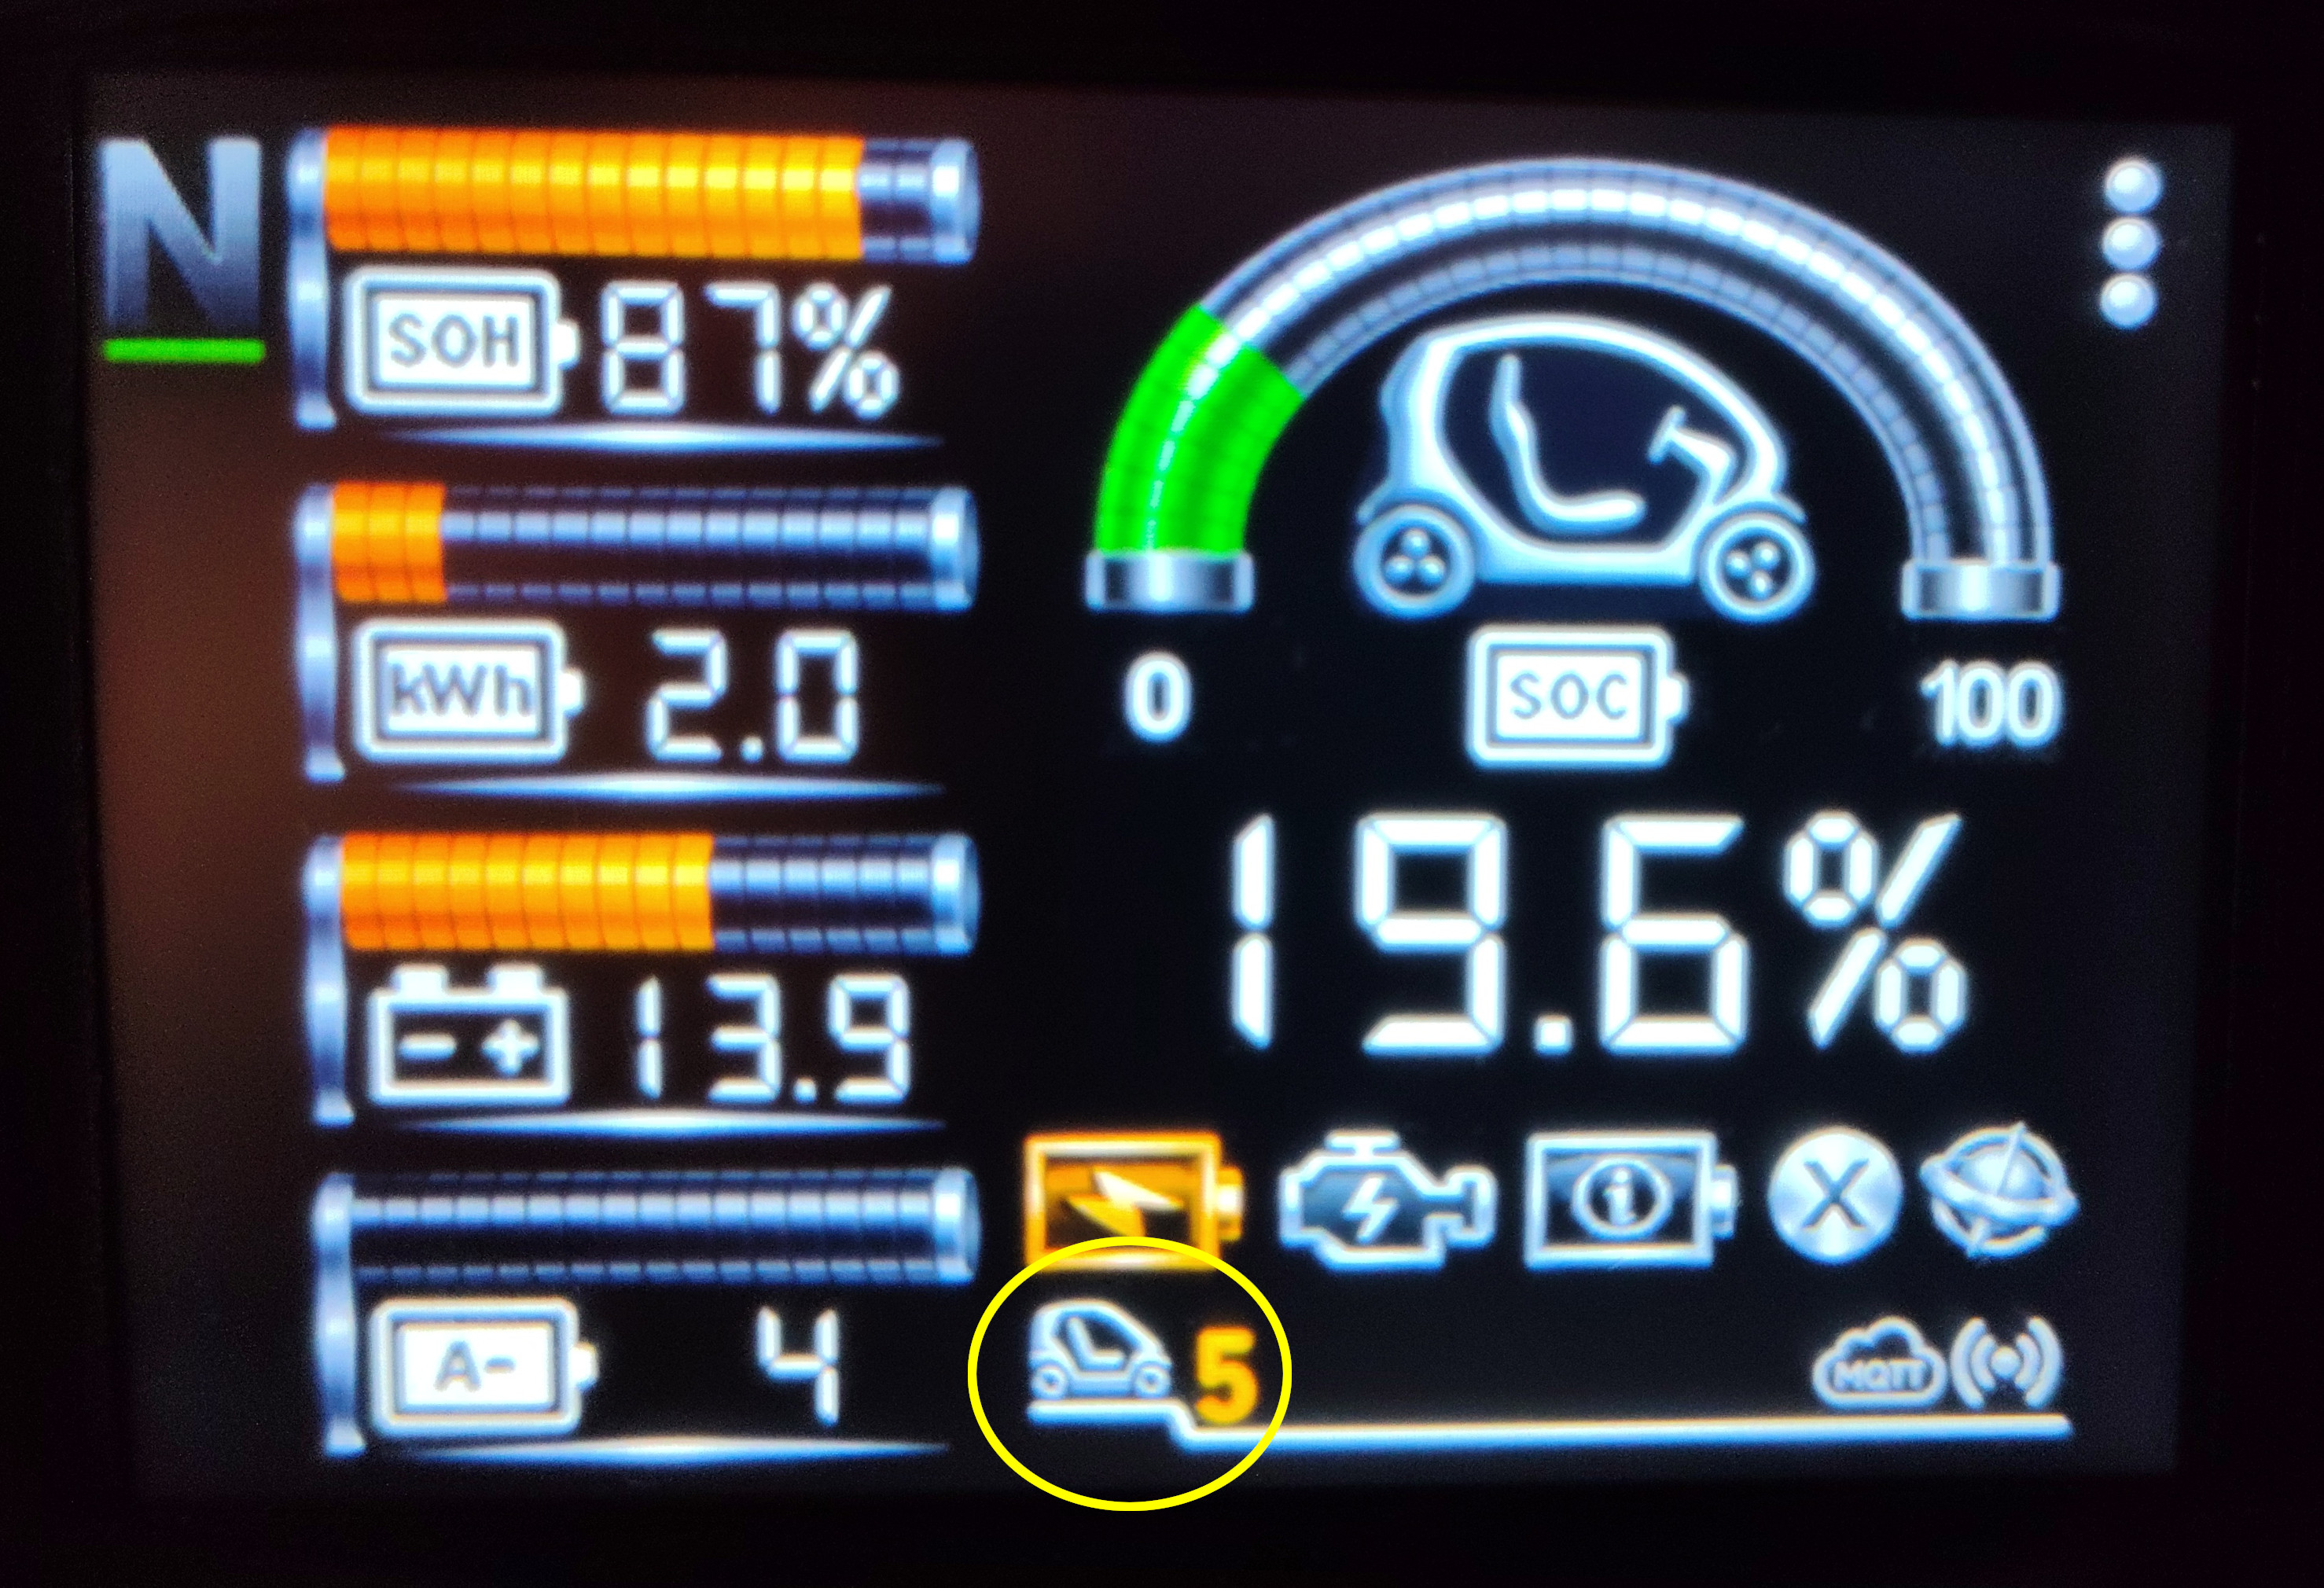
\includegraphics[width=\linewidth]{figures/trip_page_on.jpg}
        \caption{Trip recording active on trip 5.}
    \end{subfigure}
    \hfill
    \begin{subfigure}[t]{0.48\textwidth}
        \centering
        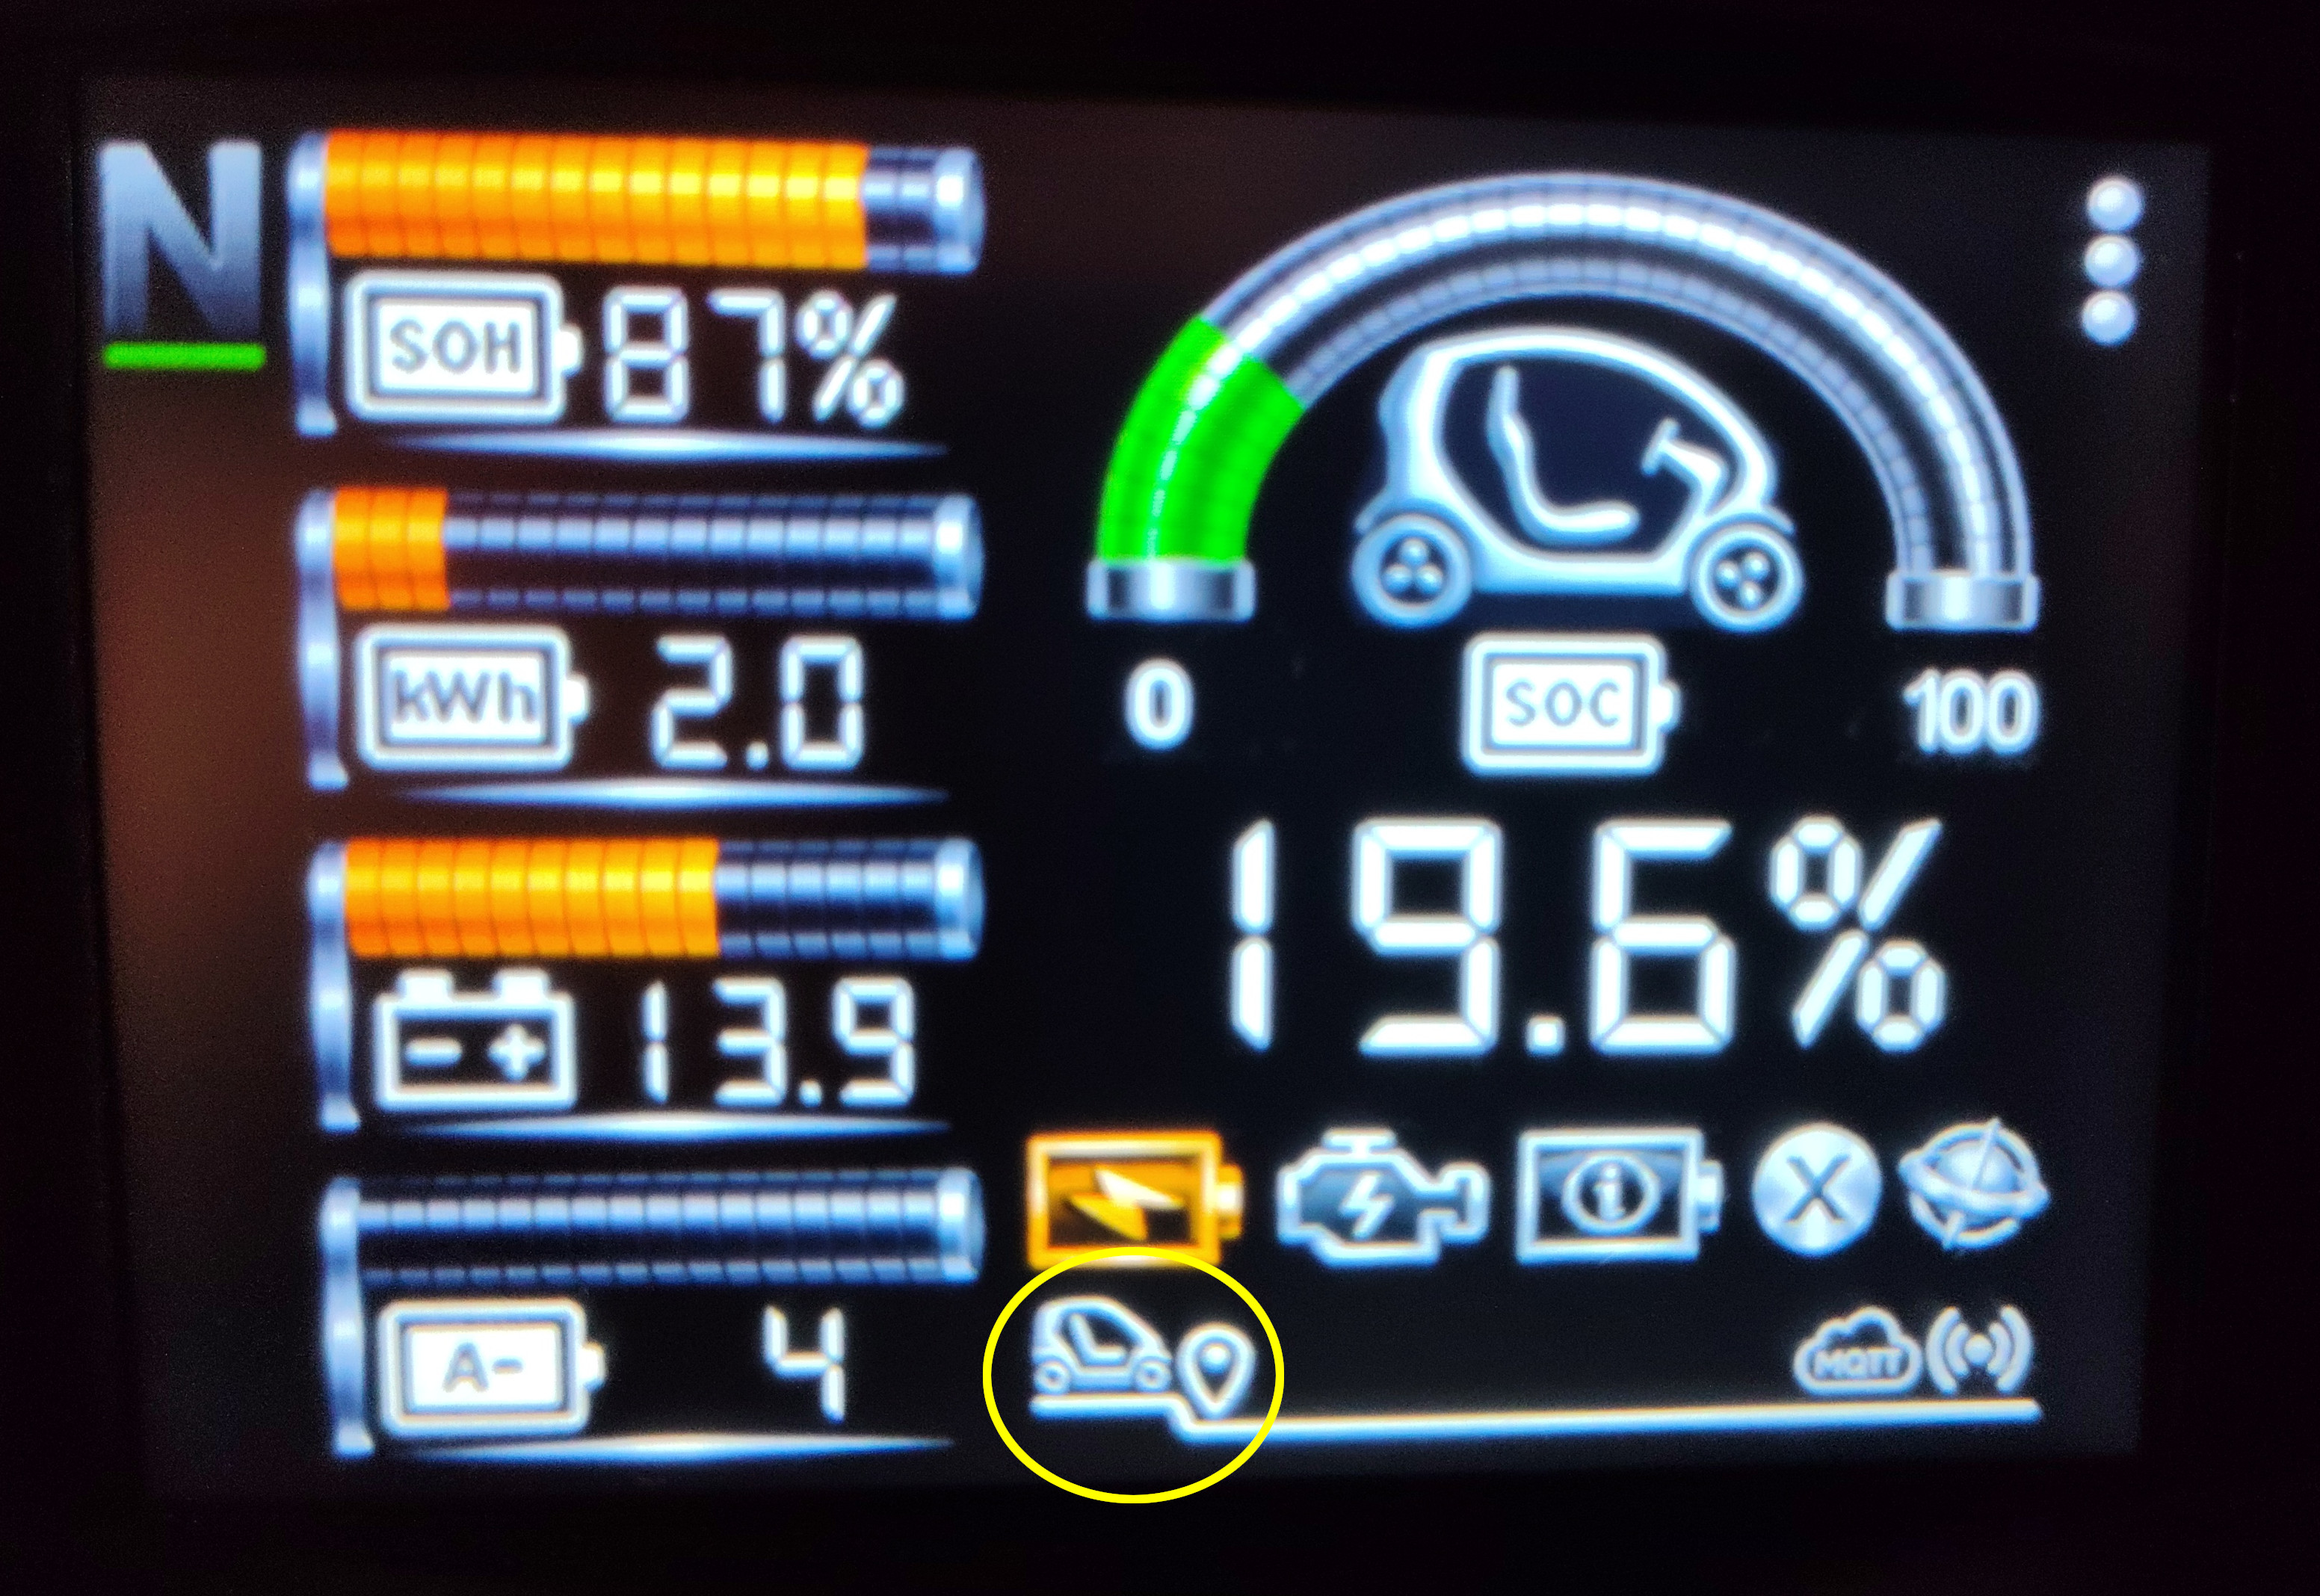
\includegraphics[width=\linewidth]{figures/trip_page_off.jpg}
        \caption{Trip recording paused.}
    \end{subfigure}
\end{figure}

Once you have released it, ToM+ changes the small trip icon showing the map symbol
instead of the trip number, to let you know it's not recording data anymore (second
picture). When you are ready to start recording the trip again, press on the trip page
until you find the desired trip cycling through all the available ones.

\subsection{Reset a trip}

If you want to clear a specific trip data you can select it and \textbf{hold down for three seconds
the trip button}. Once you have released it, you should notice that all trip values in
the page were reset (tipically to zero). The difference between this action and the previous 
one is that in this case the trip data is cleared, while in the previous one the trip data is just paused.
In addition, here you need to be on the trip page, while in the previous one you should be on any other page.

\clearpage

\section{The trip history page}
\label{sec:trip_history}

This page stores the data of the last twenty trips and the layout is the same as the alarm log page.
The values are updated and stored only when the selected trip is the \textbf{number 5}.

\subsection{How to access the trip history page}

This page is not accessible from the main page, but you can reach it by \textbf{long pressing 
the alarm log icon} (i.e. the fourth one) in the bottom line of the screen until it changes. This is because the trip history page
is not a page you will use often, so it was decided to hide it from the main page
to save space, as well as the error page. So, the sequence of pages available by \textbf{long pressing the alarm log icon} are:
alarm log page (Section~\ref{sec:alarm_log}) $\rightarrow$ error page (Section~\ref{sec:error_page}) $\rightarrow$ trip history page $\rightarrow$ back to alarm log page,
each one with the respective icon. Next time ToM+ turns on, trip history page will be the default fourth icon.\\

\begin{figure}[H]
    \centering
    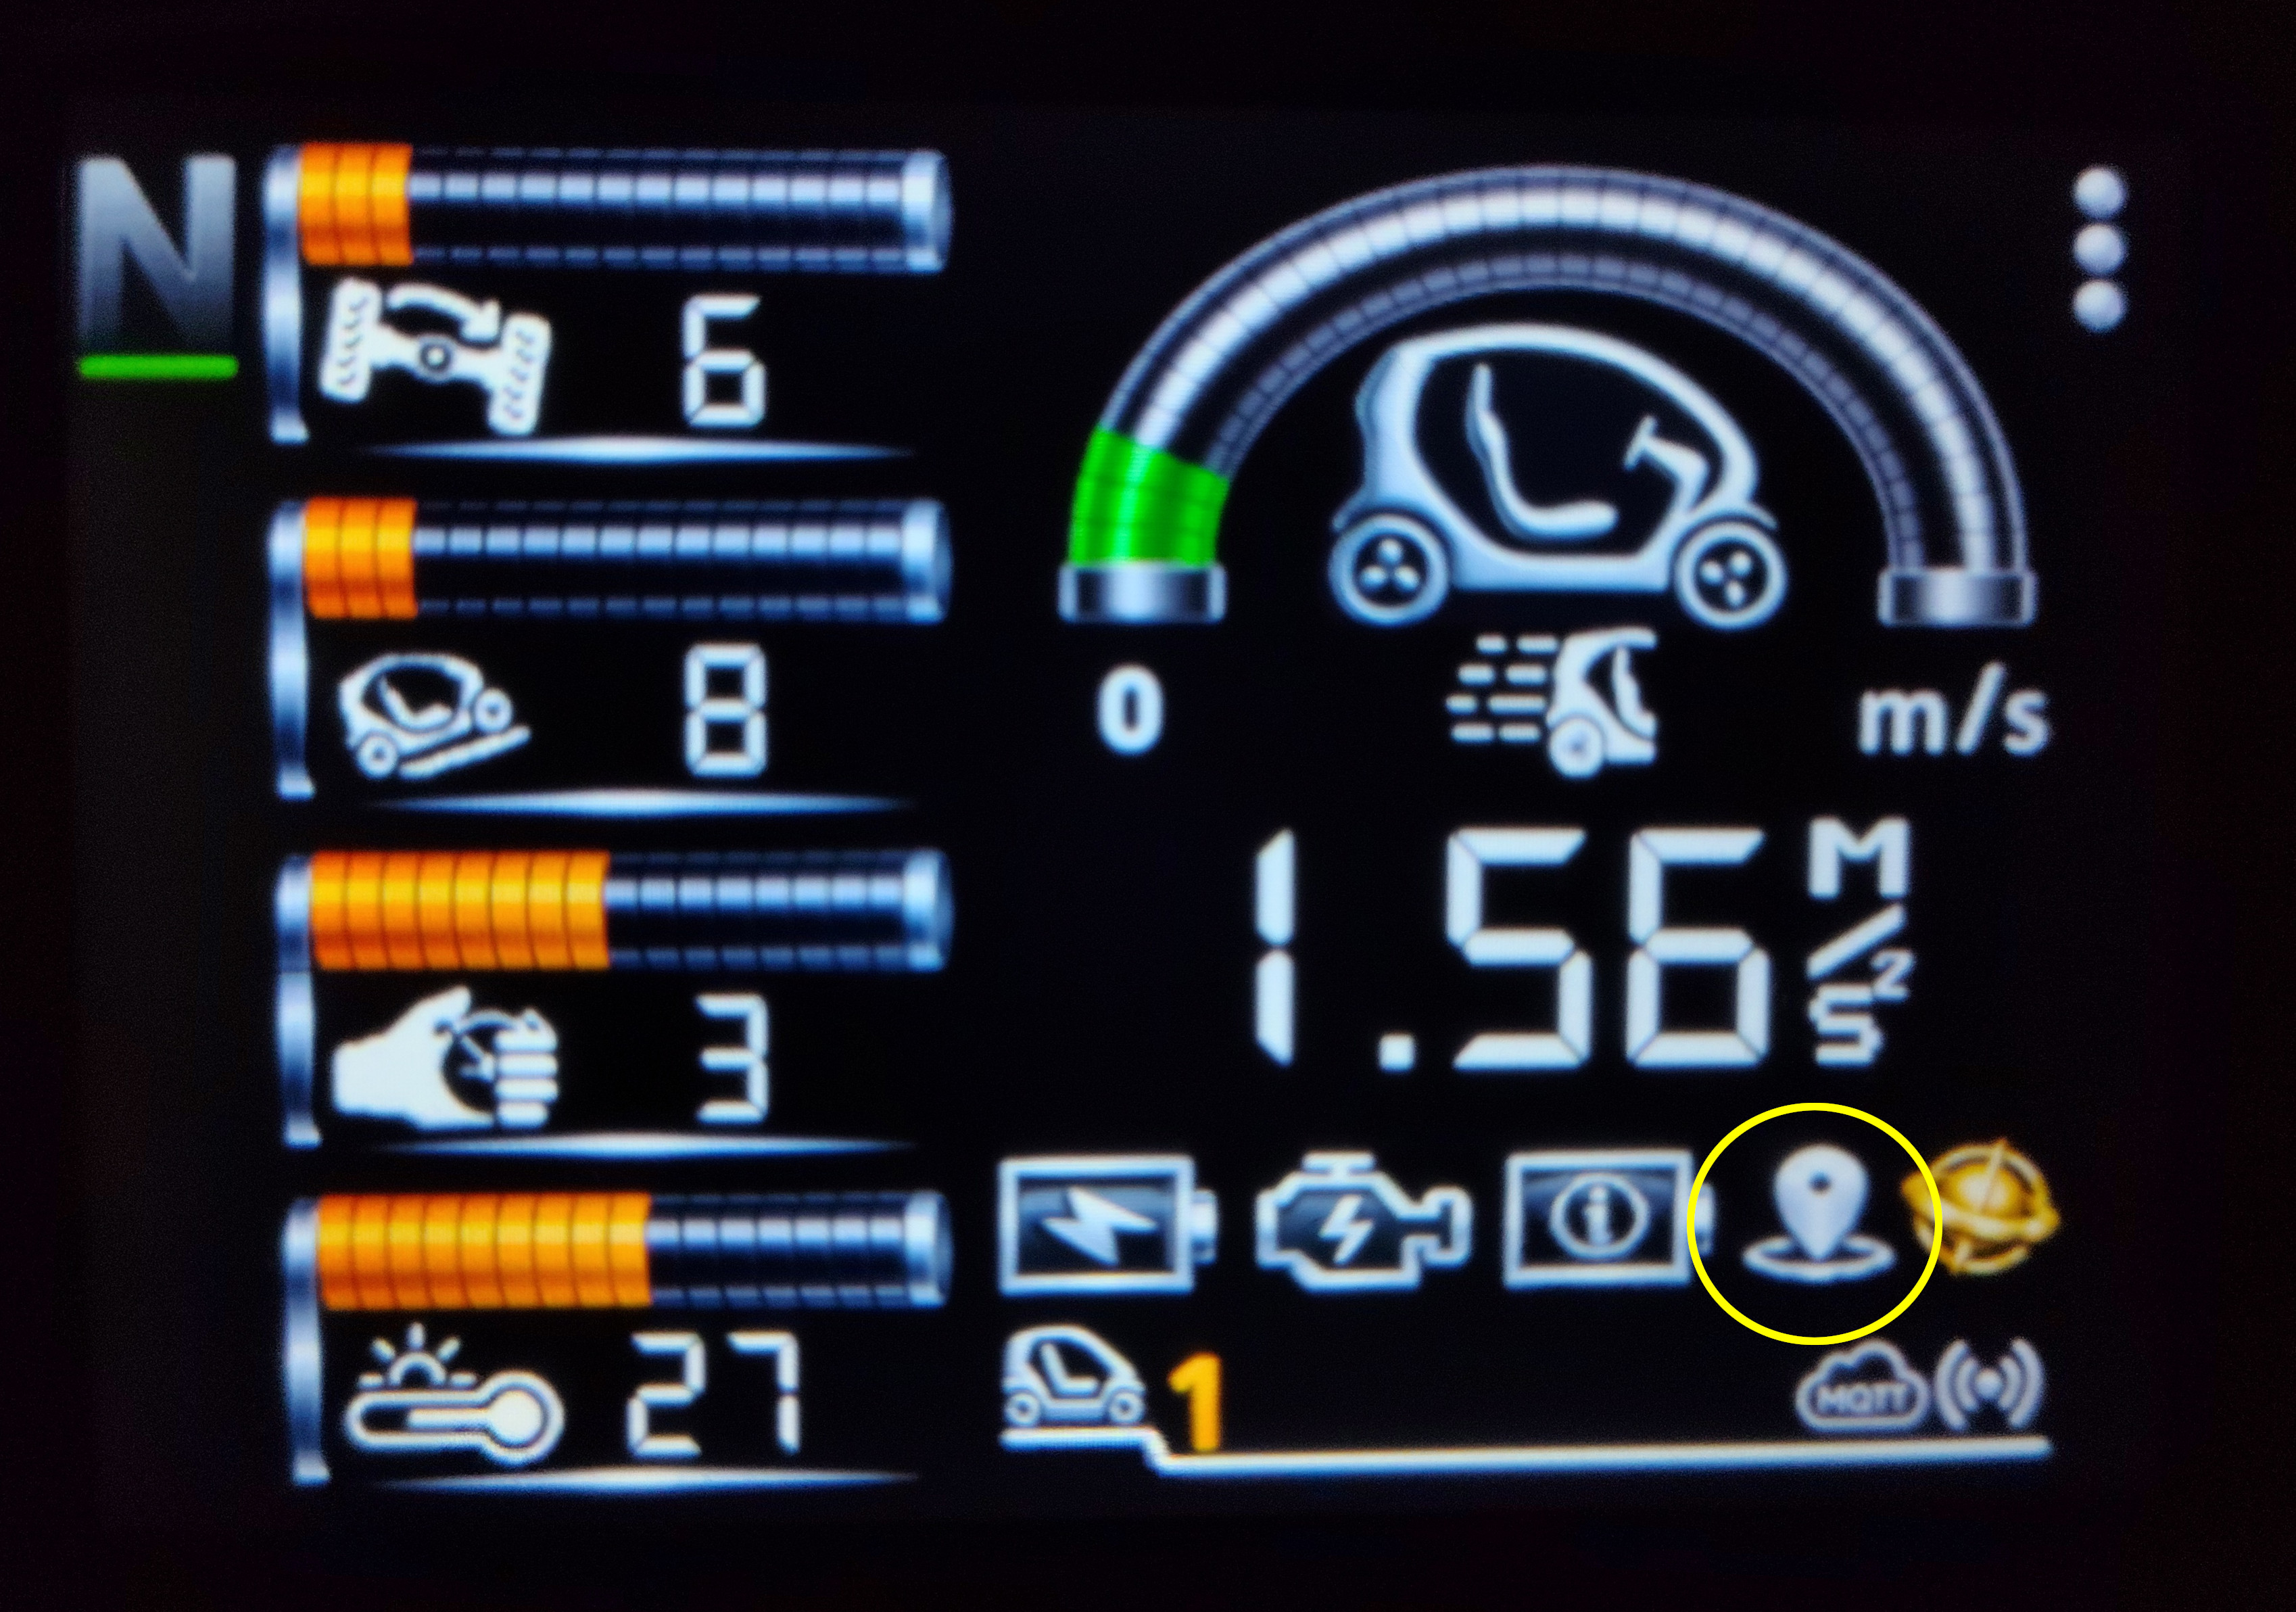
\includegraphics[width=0.8\textwidth]{figures/enter_trip_log_page.jpg}
    \caption{The icon to access the trip history page.}
\end{figure}

\subsection{Main trip history page controls}

\begin{figure}[H]
    \centering
    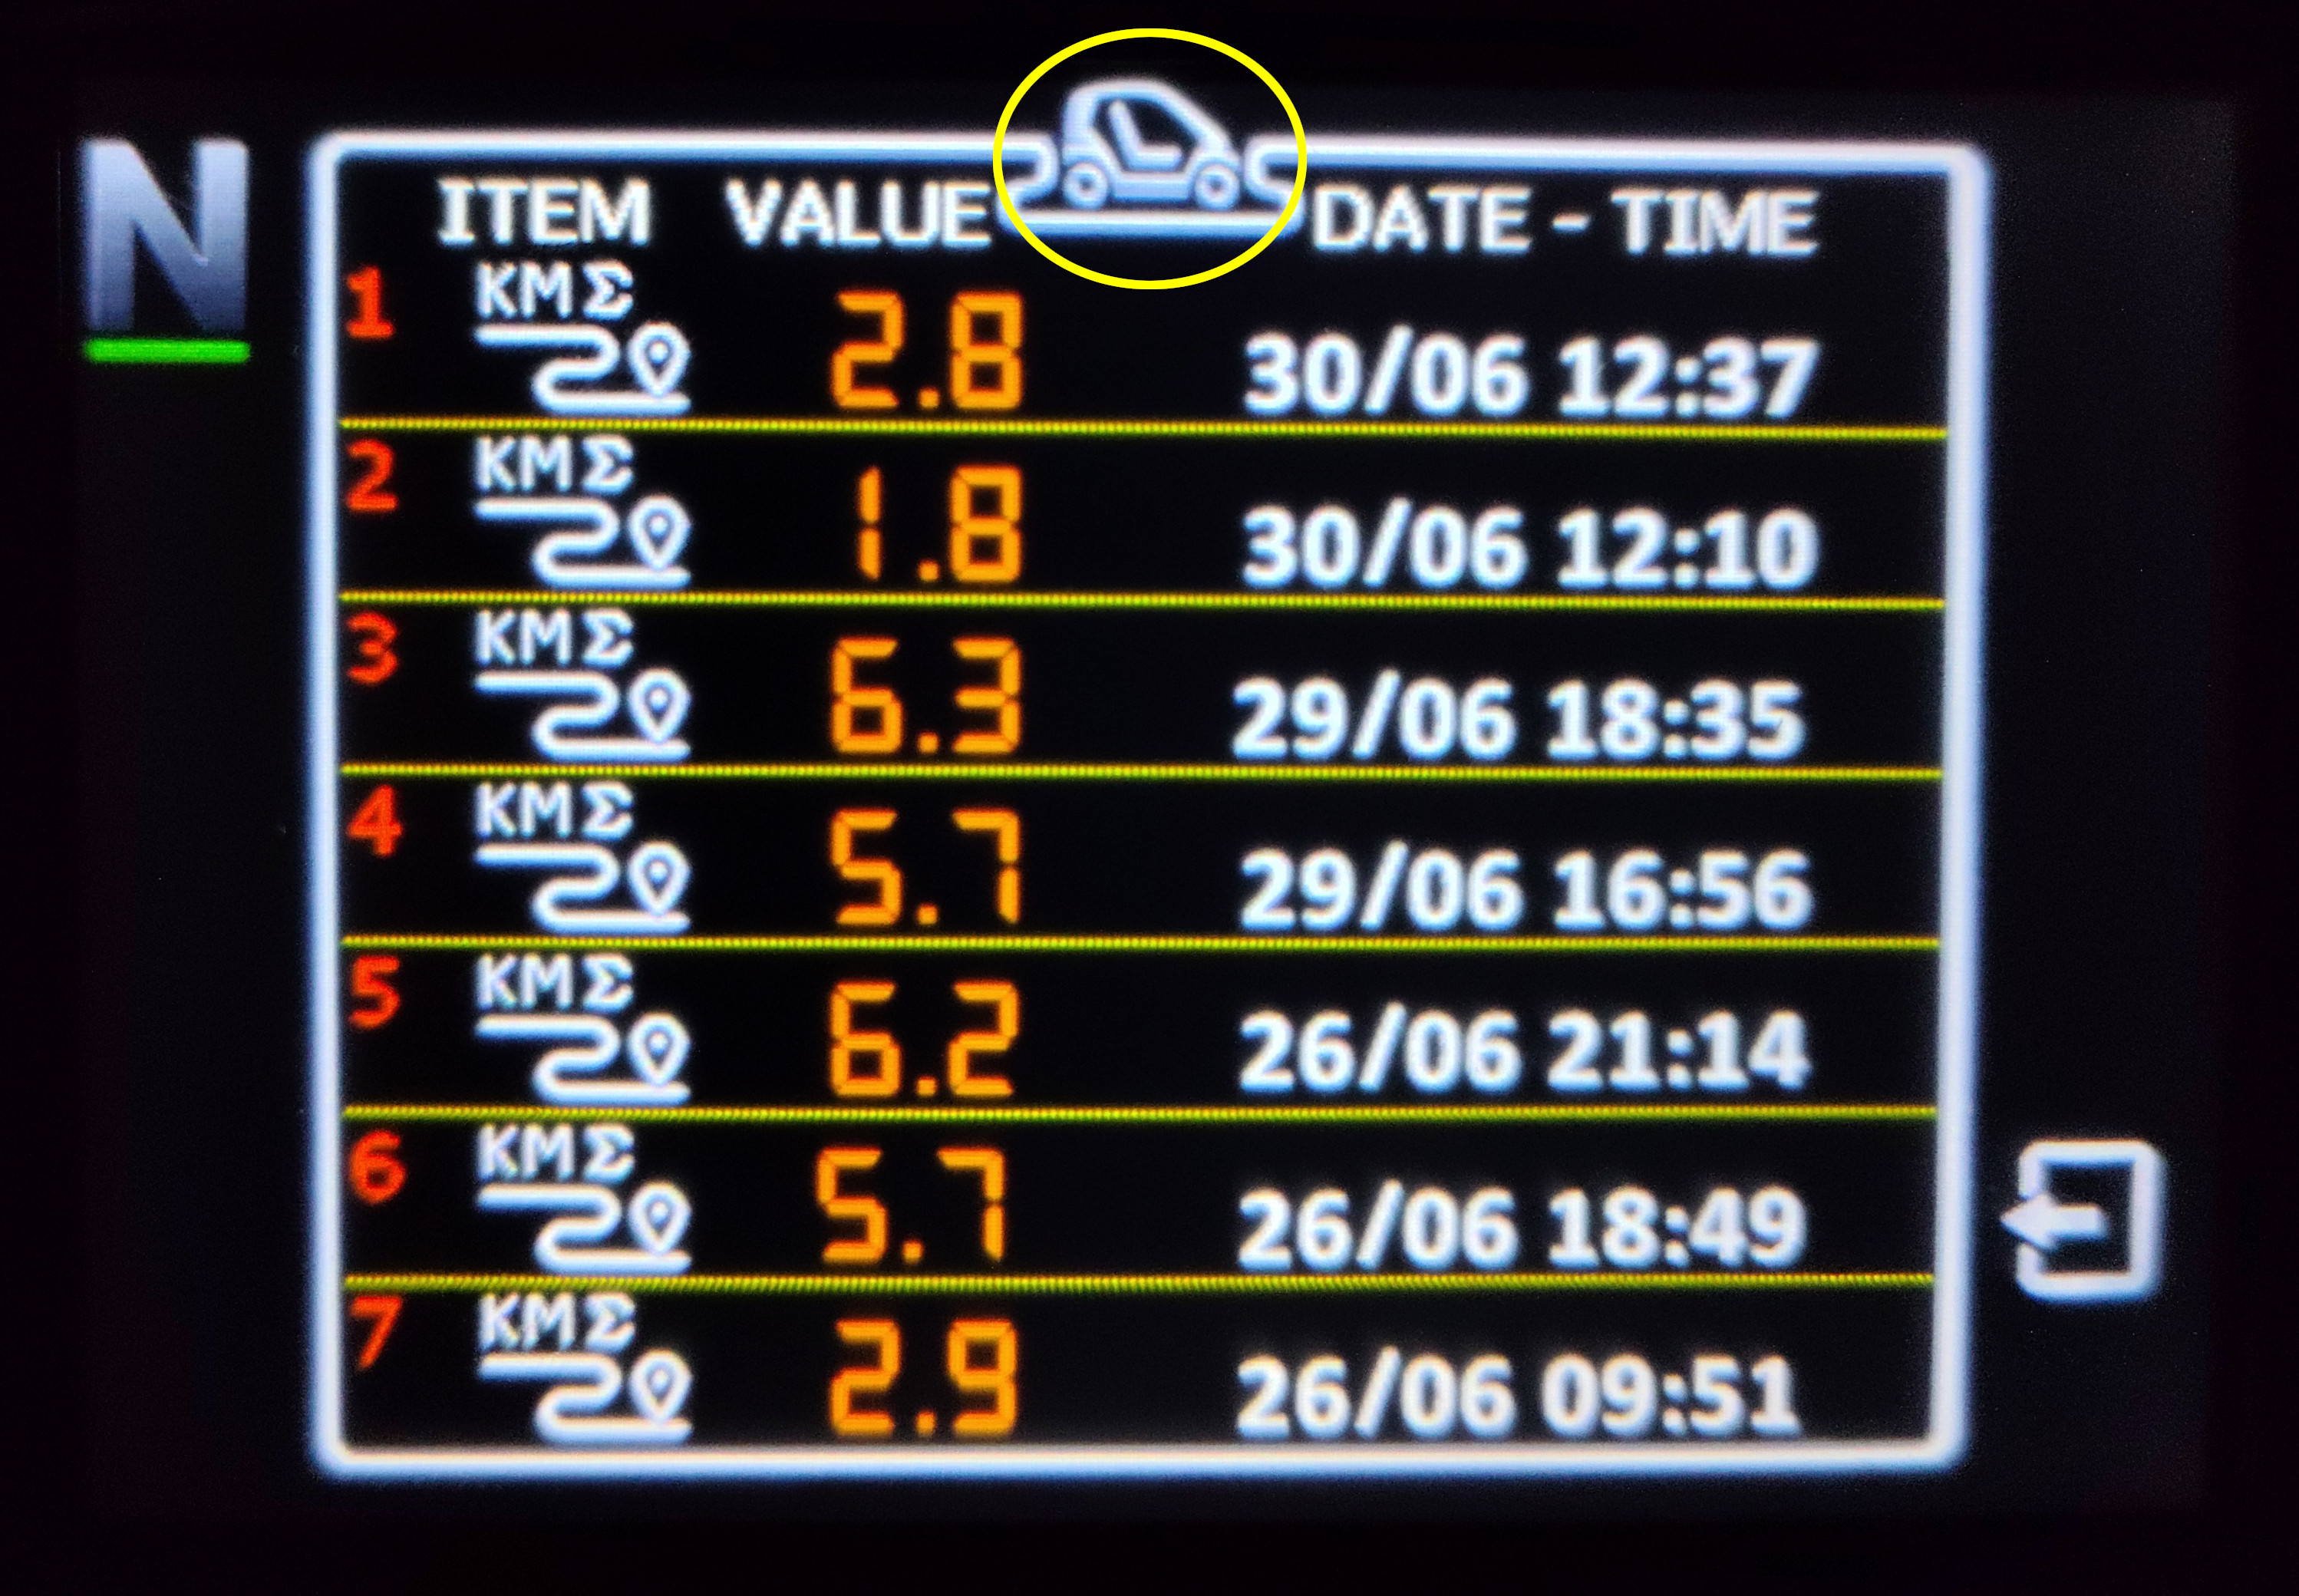
\includegraphics[width=0.8\textwidth]{figures/trip_history_page.jpg}
    \caption{The trip history page.}
\end{figure}

In this image you can see the first seven trips stored in the list, with their date and time, the distance traveled.
You can easily change the data shown on each row by pressing on the icon of the data as shown below.
The data will cycle between most of the trip data available, so you can choose which one to show. 
In the next images you can see the same page with the trip power consumption and average speed.

\begin{figure}[ht]
    \centering

    \begin{subfigure}[t]{0.48\textwidth}
        \centering
        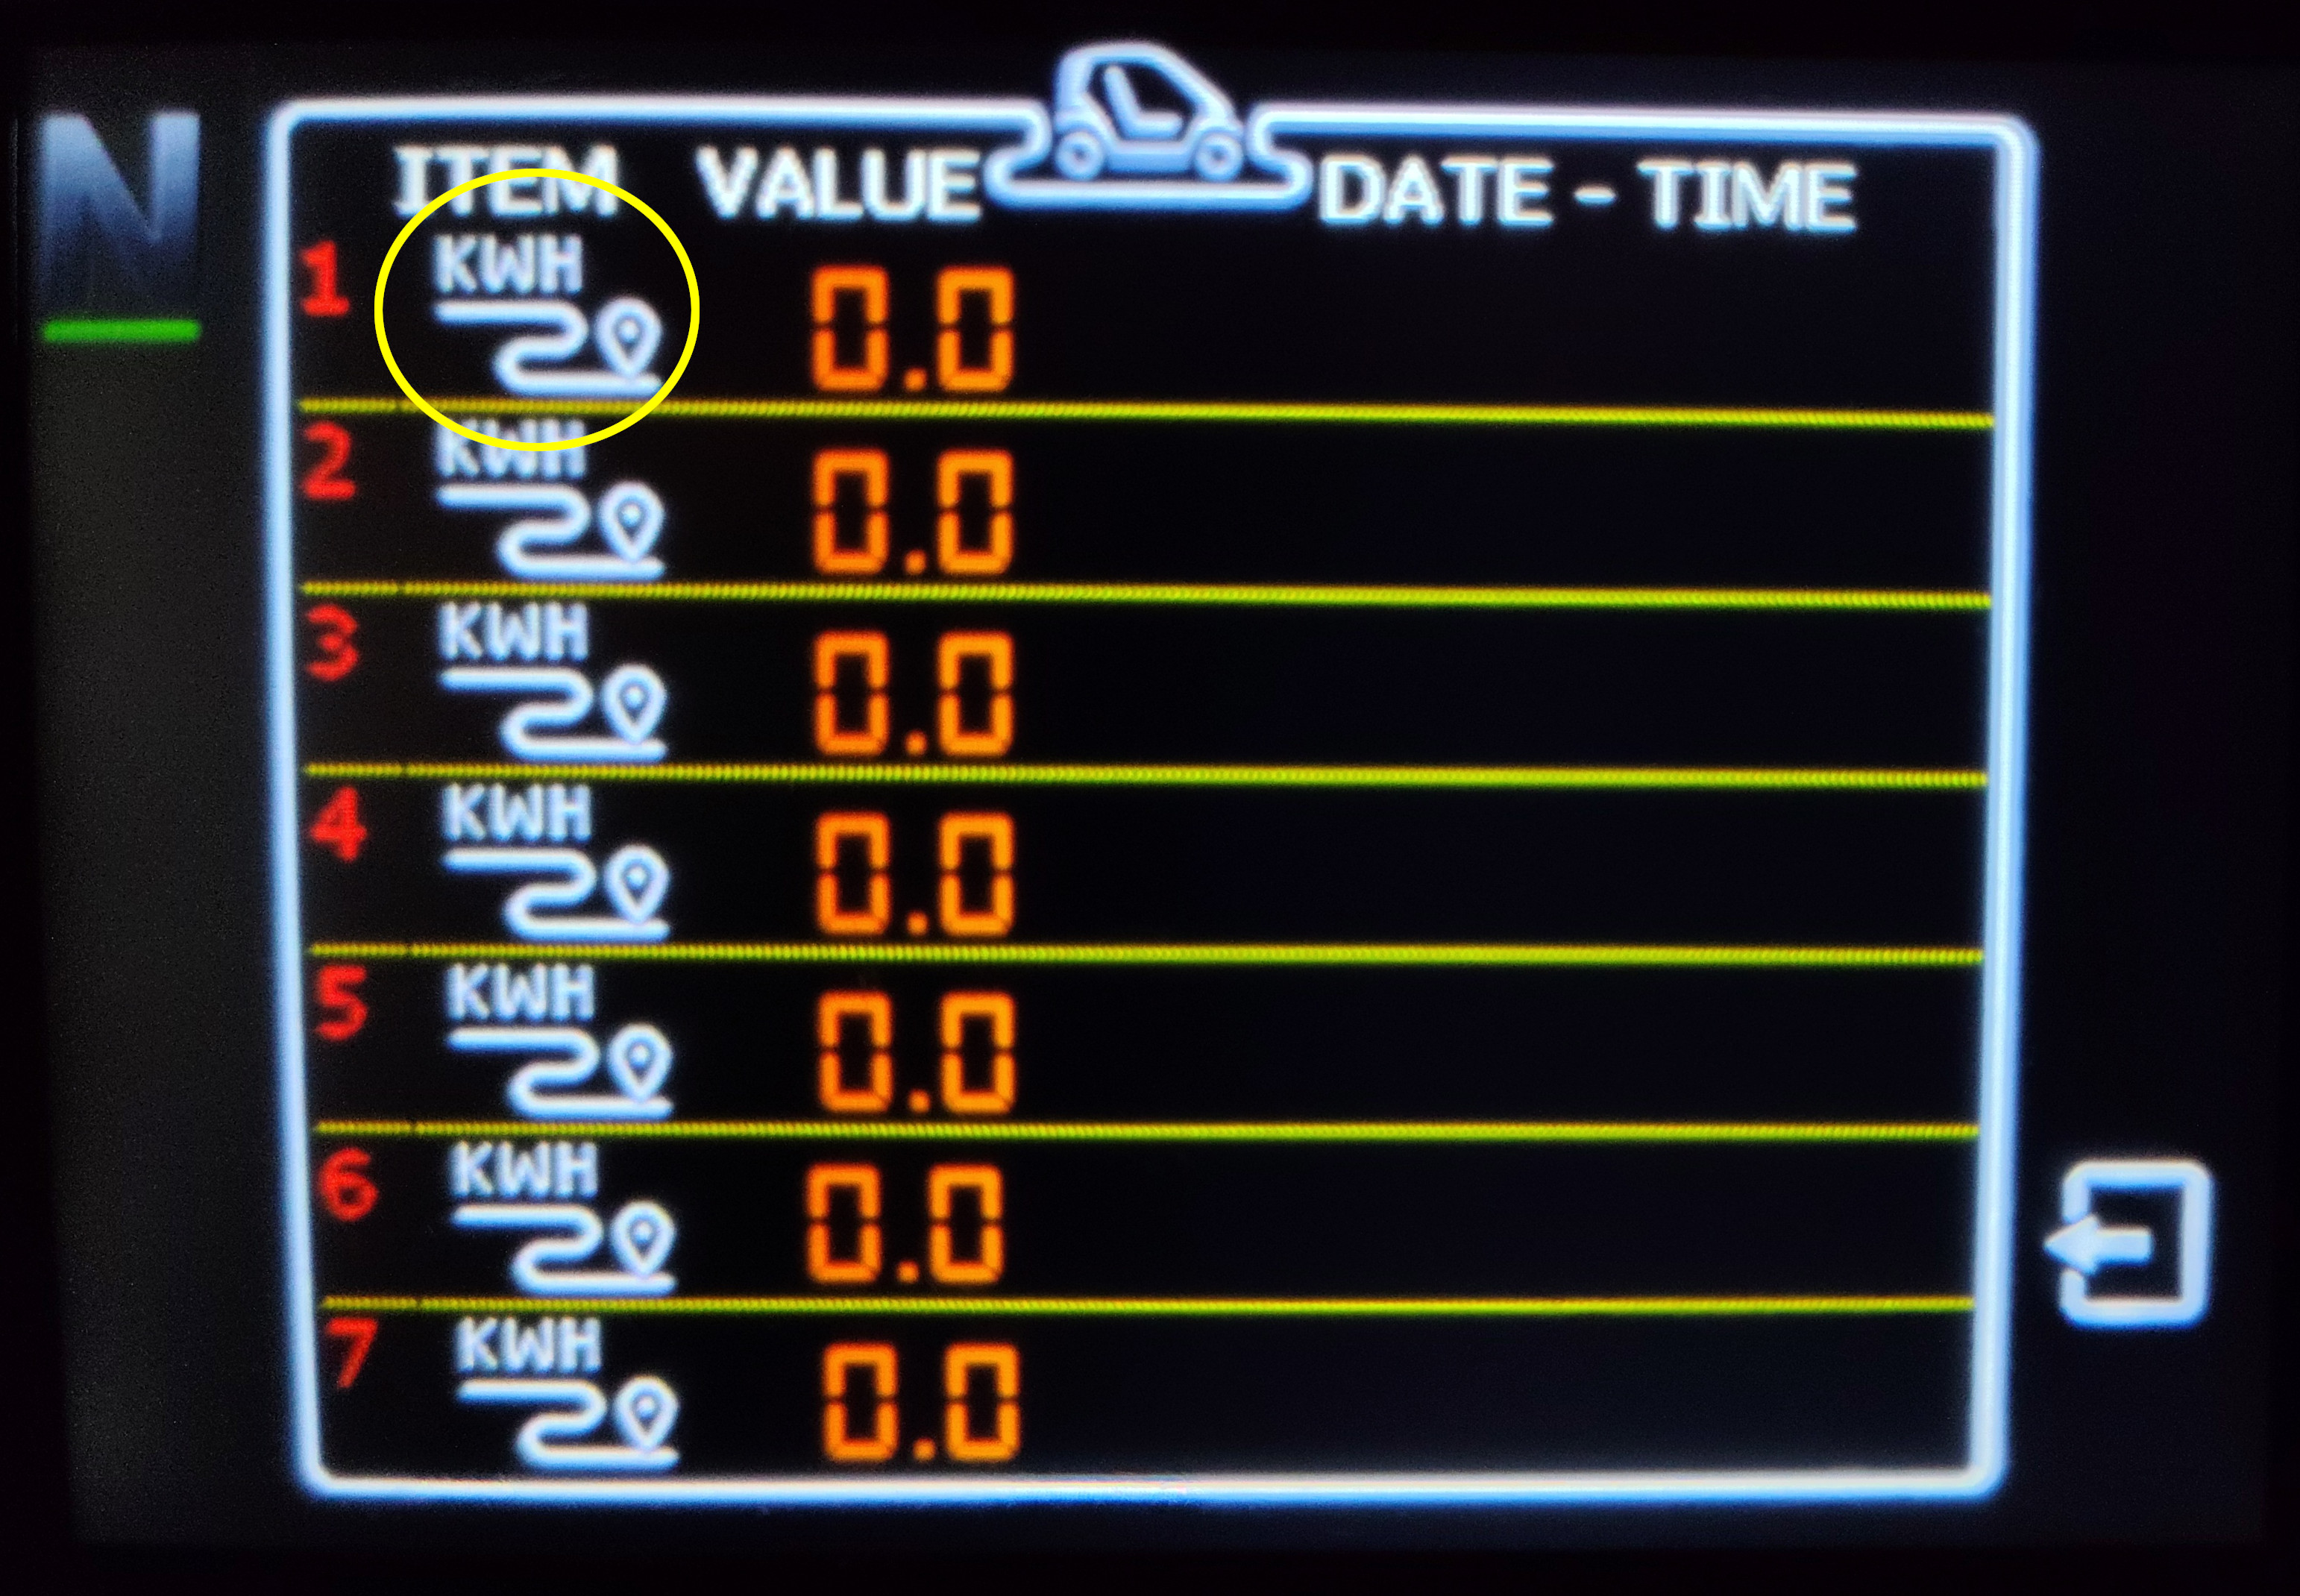
\includegraphics[width=\linewidth]{figures/trip_log_kwh.jpg}
        \caption{Showing trip power consumption.}
    \end{subfigure}
    \hfill
    \begin{subfigure}[t]{0.48\textwidth}
        \centering
        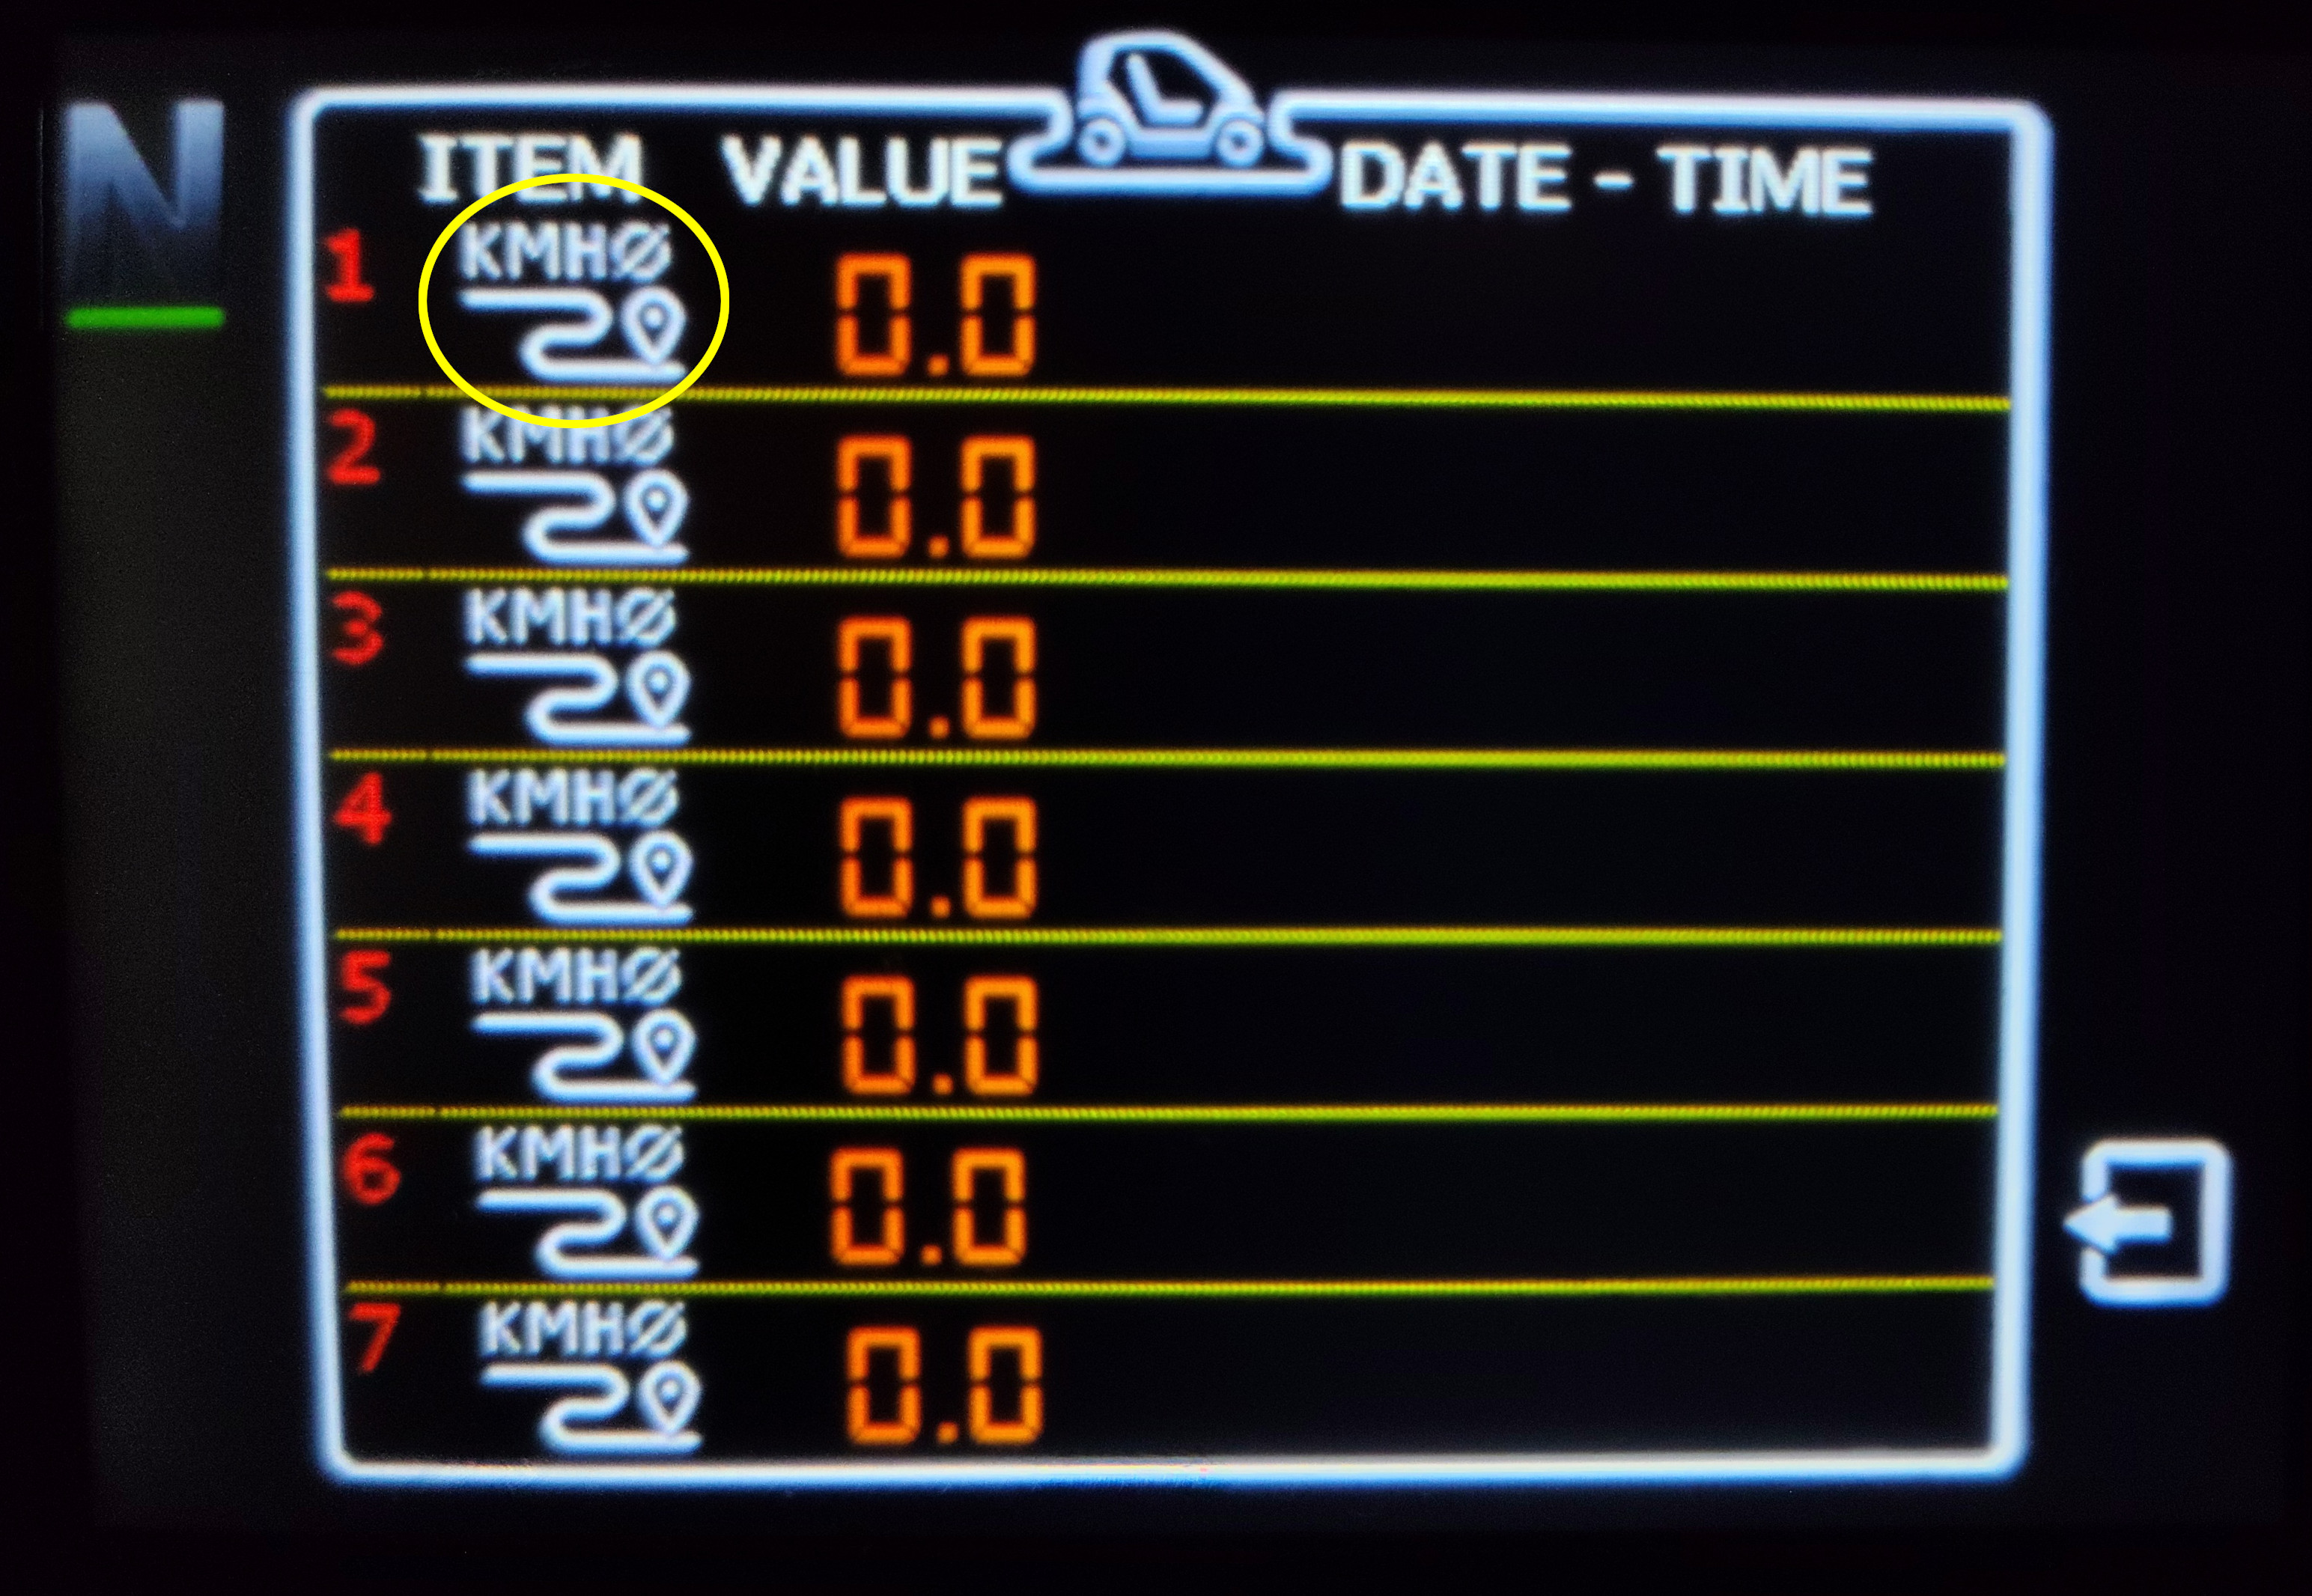
\includegraphics[width=\linewidth]{figures/trip_log_kmh.jpg}
        \caption{Showing trip average speed.}
    \end{subfigure}
\end{figure}

On the web server you can see all of them at once, it will be discussed in Section~\ref{sec:web_trip_history}.

\clearpage

\section{The error page}
\label{sec:error_page}

This page is similar to the alarm log page and the trip history page, but it will show you the last DTC errors that occurred.
The controls to delete records or to see older ones was already discussed in Section~\ref{sec:alarm_log}

\subsection{How to access the error page}

This page is not accessible from the main page, but you can reach it by \textbf{long pressing 
the alarm log icon} (i.e. the fourth one) in the bottom line of the screen until
it changes. As we discussed before, the sequence of pages available by long 
pressing the alarm log icon are: alarm log page (Section~\ref{sec:alarm_log}) 
$\rightarrow$ error page $\rightarrow$ trip history page (Section~\ref{sec:trip_history})
$\rightarrow$ back to alarm log page, each one with the respective icon. 
Next time ToM+ turns on, error page will be the default fourth icon.\\

\begin{figure}[ht]
    \centering

    \begin{subfigure}[t]{0.48\textwidth}
        \centering
        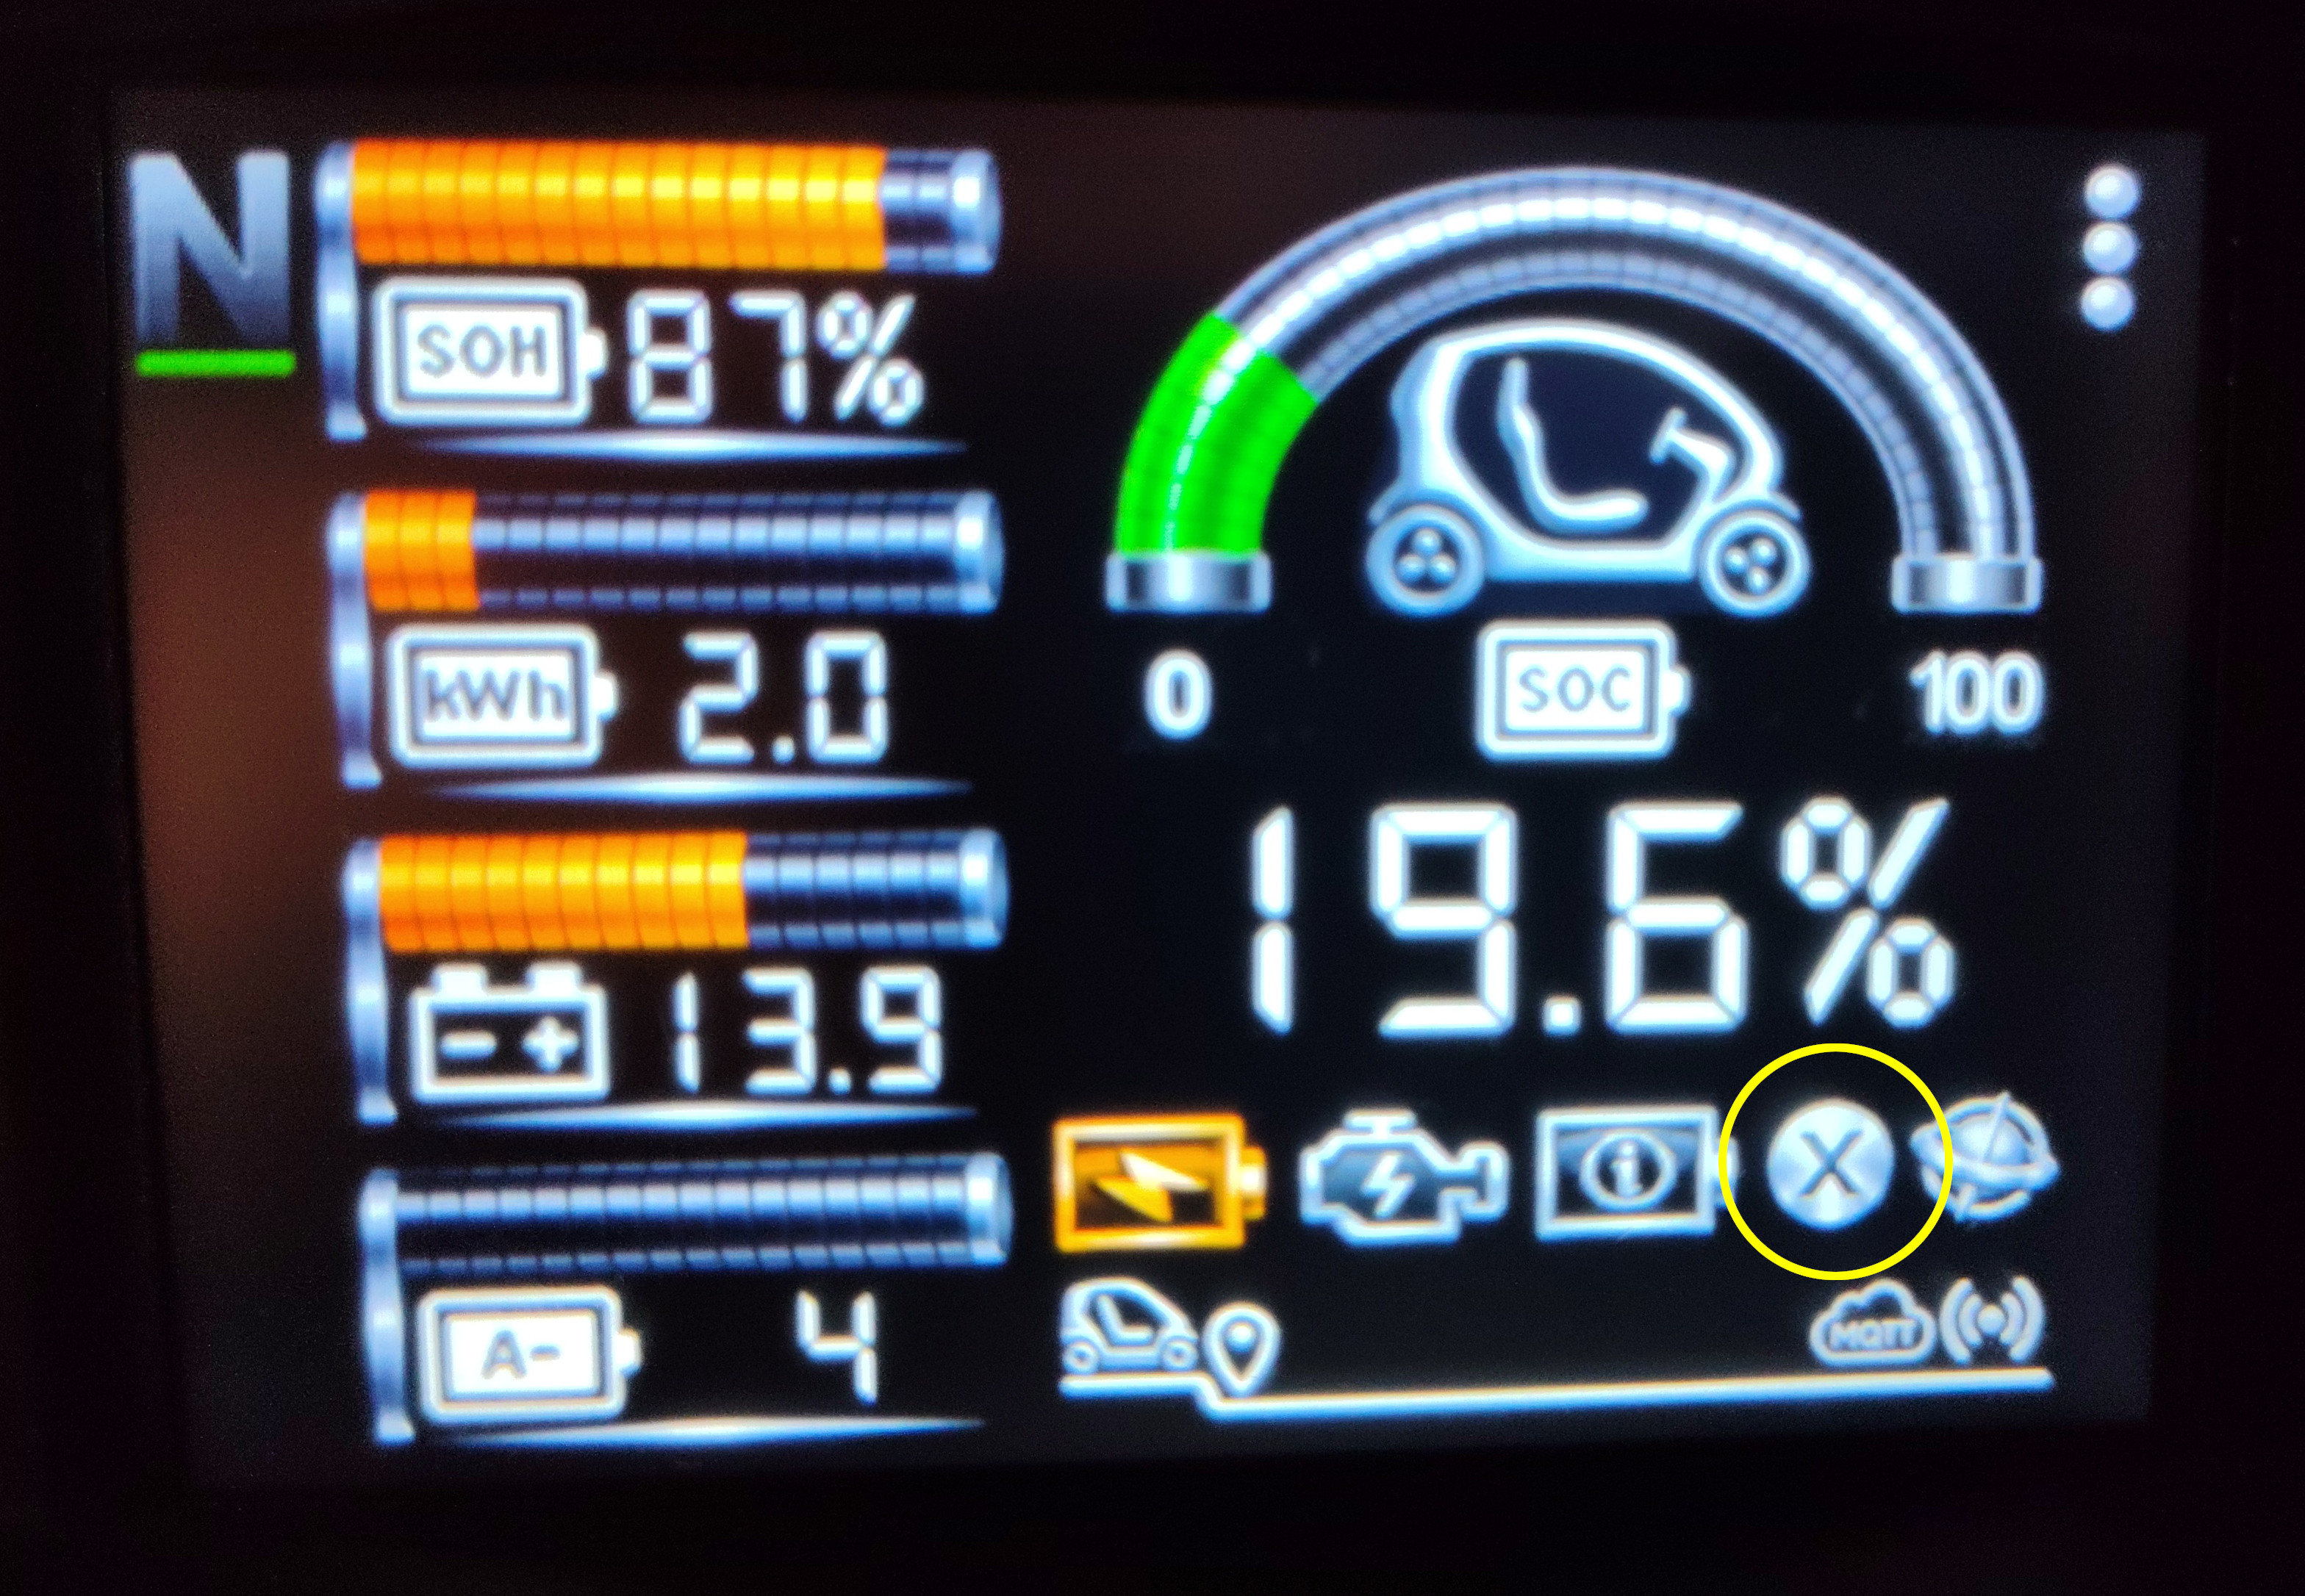
\includegraphics[width=\linewidth]{figures/enter_error_page.jpg}
        \caption{The icon to access the error page.}
    \end{subfigure}
    \hfill
    \begin{subfigure}[t]{0.48\textwidth}
        \centering
        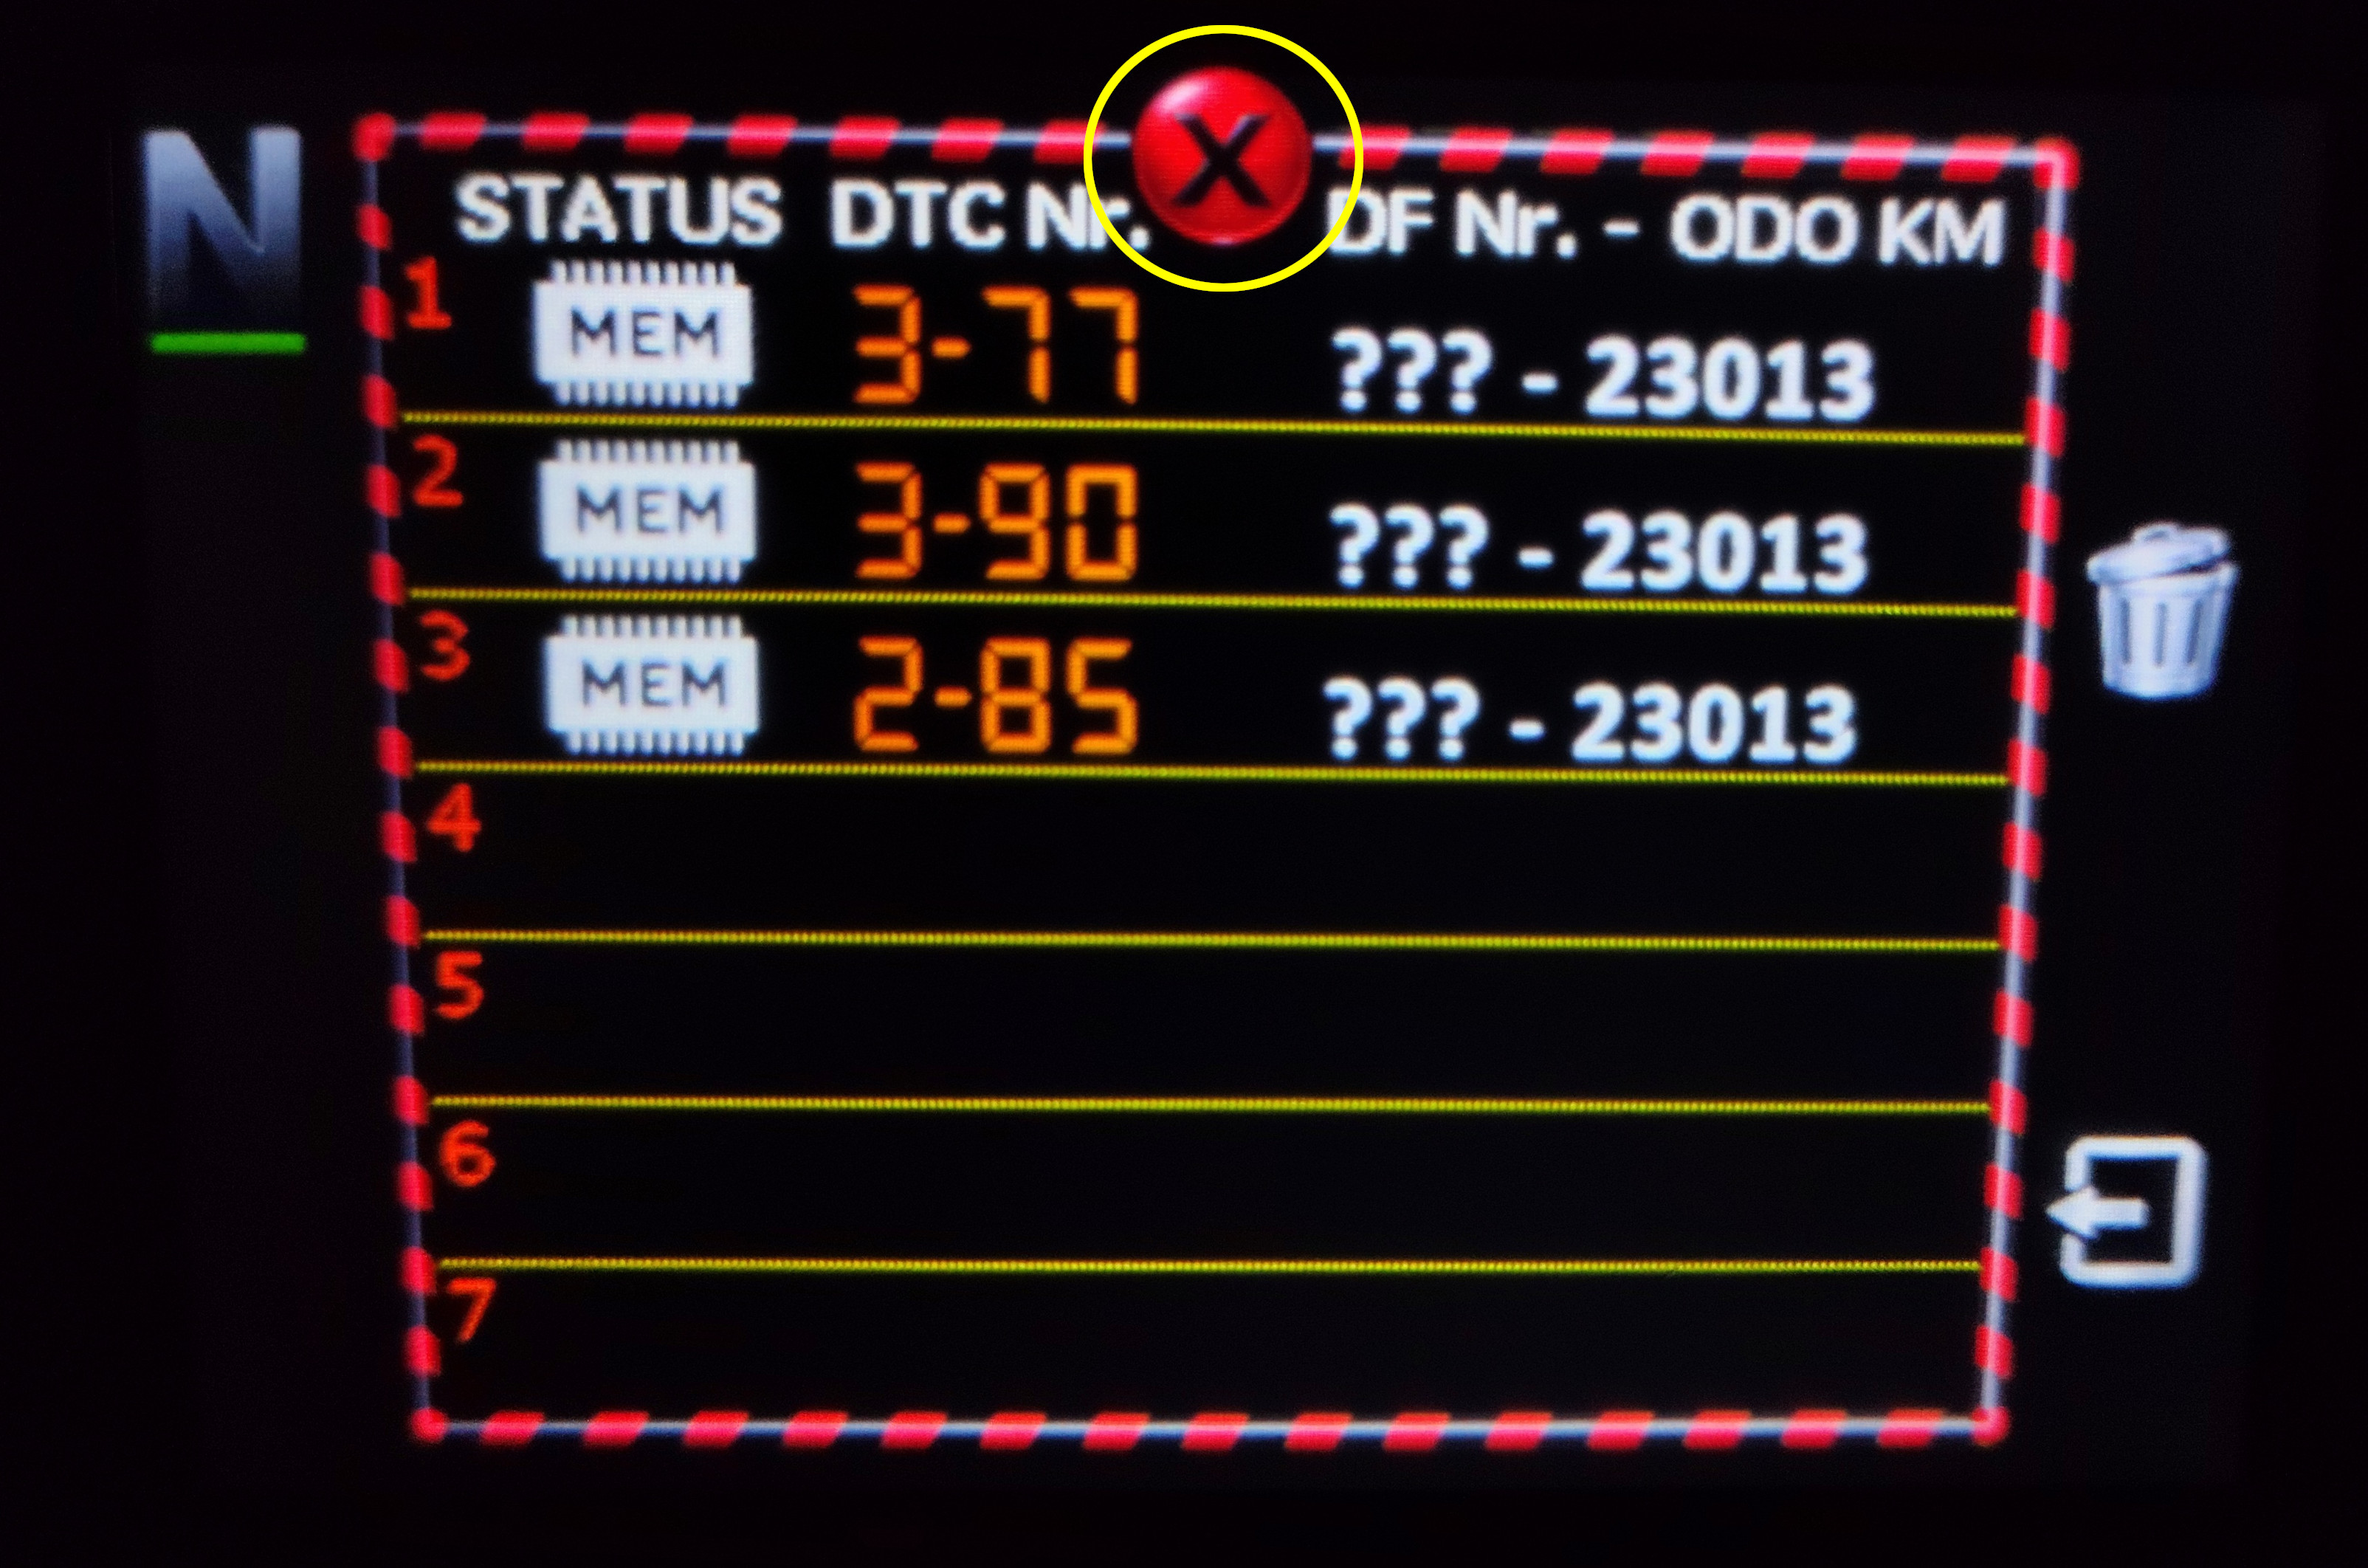
\includegraphics[width=\linewidth]{figures/error_page.jpg}
        \caption{Showing the error page.}
    \end{subfigure}
\end{figure}

\subsection{Main error page controls}

As you can see in the second image above, the error page is similar to the alarm log page. 
It shows a list of the last 14 errors that occurred, with their ODO, the DTC number,
the DF number if available, and a representative icon. Refer to the relative page on
the web server for more information such as SOC, speed and a brief description (Section~\ref{sec:web_diagnostic}).\\

By pressing on the icon of the error (circled in yellow in the image) you can cycle between the pages of stored errors,
which are 14 in total. The first page shows the last 7 errors, while the second page shows the older ones.
To \textbf{delete error records} both in this page and on the car, simply click on the trash can icon.\\

To enable DF numbers and descriptions please refer to Section~\ref{sec:add_wifi_profile}.
If DF numbers are shown (instead of \textit{???}) you can press that number to
have \textbf{additional description} about the pressed error. The seventh line will be
replaced by this additional info and you can click on it to hide again.\\

As in other pages the space wasn't enough to put the buttons to change page, so you can press
the exit button in the bottom right corner to go back to the previous page and then change the active one if you want.

\clearpage

\section{The charging page}
\label{sec:charging_page}

This page doesn't show while driving and there isn't a specific button to view it. That
is mainly because this charging screen appears automatically when Twizy is currently
in charge state. 

As you can see in the image the layout is the same as the dashboard page. The current
SOC is shown in the center replacing the speed value.\\

An animation will start as well, with a different speed depending on the charging power level.
In the photo below there are also some charging specific data, which you can change in the settings
as it will be explained later. In this page you don't have the icons status bar, but you still
have the network status icons in the bottom right corner, since you can monitor your car charging
values when the car is powered off too. In fact, ToM+ will power on automatically when you plug your
Twizy into a valid power supply.

\begin{figure}[H]
    \centering
    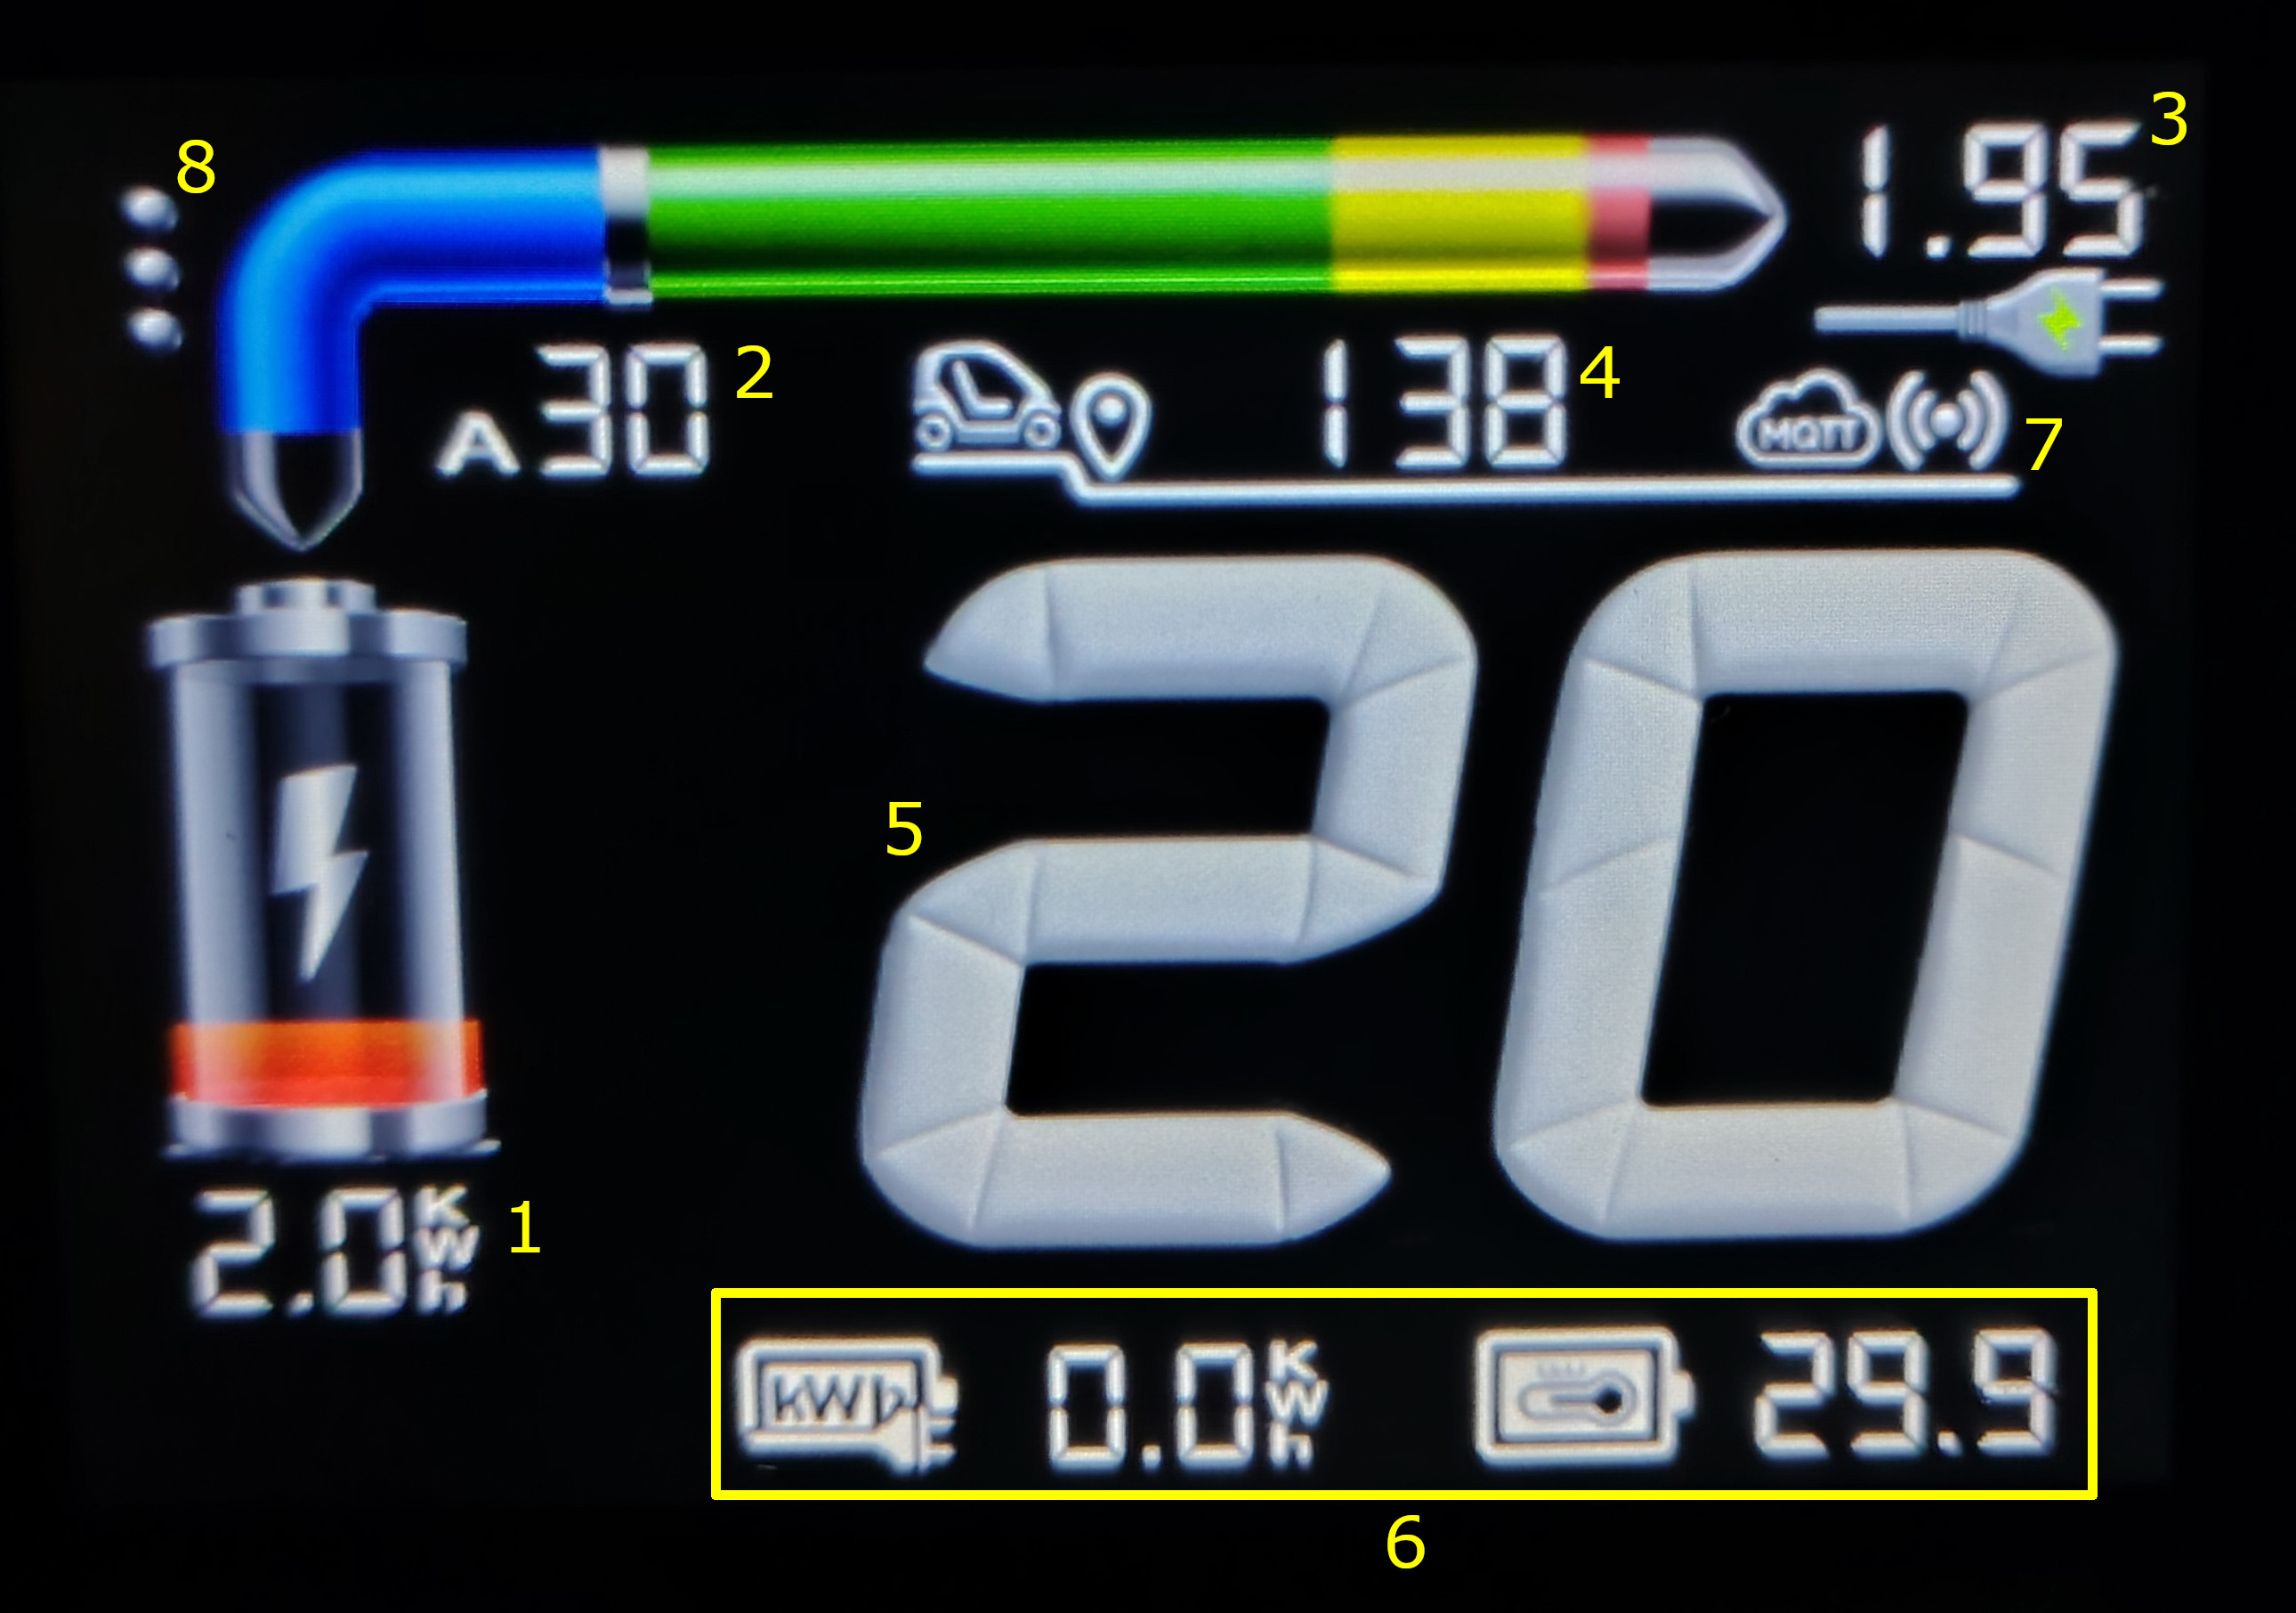
\includegraphics[width=0.8\textwidth]{figures/charging_page.jpg}
    \caption{The charging page.}
\end{figure}

\begin{description}
\item[\textbf{1}] Current power stored in the battery, expressed in \(kWh\).
\item[\textbf{2}] A value chosen from torque, power consumption and current consumption, which is used to fill
the blue part of the power bar. Tap on the value to cycle between the three options.
\item[\textbf{3}] Current charging power, expressed in \(kW\), used to fill the right side of the power bar.
\item[\textbf{4}] Shows the ETA, i.e., the estimated time to complete charging.
\item[\textbf{5}] The current SOC, i.e., the state of charge of the battery, expressed in \%.
\item[\textbf{6}] Additional displayed values, you can cycle between them by tapping on the icon to change.
\item[\textbf{7}] Icons for MQTT and WiFi. Greyed out when disconnected, and colored when connected. Tap on the icons if you want to perform a new WiFi scan or a MQTT reconnection.
\item[\textbf{8}] Shortcut button to open the settings page, to access more advanced settings.
\end{description}


\section{The settings page}
\label{sec:settings_page}

In order to let ToM be much more customizable here is the settings page, accessed by
pressing the three dots on the top right corner in any of the main pages. Now you can
easily edit the basic appearance of your personal ToM.

\begin{figure}[H]
    \centering
    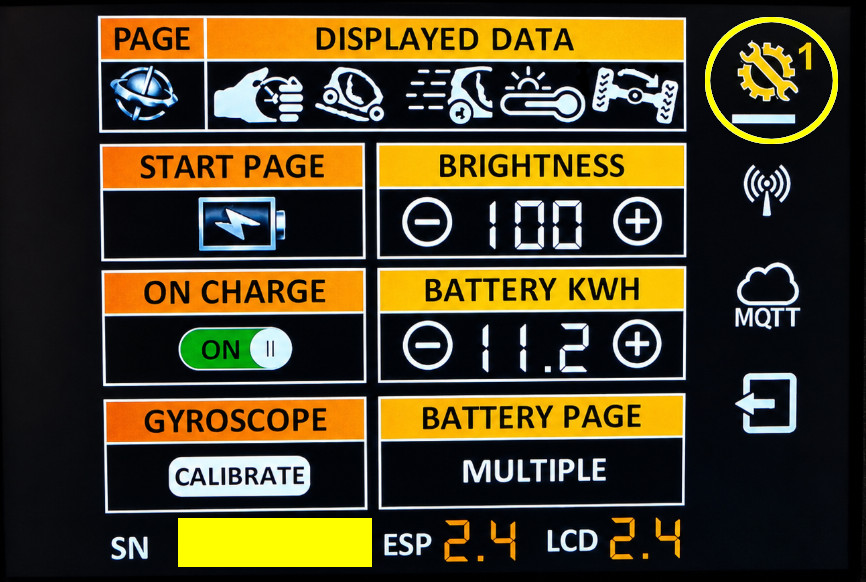
\includegraphics[width=0.8\textwidth]{figures/settings_page1.jpg}
    \caption{The first settings page.}
    \label{fig:settings_page}
\end{figure}


\noindent The last row will give you info about your personal ToM and will display:
\begin{itemize}
    \item Your ToM \textbf{Serial Number} in the first field (it's censored in the figure above)
    \item The black box (ESP) firmware version (currently 2.4 in the figure)
    \item The LCD touch display firmware version (currently 2.4 in the figure)
\end{itemize}
You can update to the latest version of the firmware as explained in Section~\ref{sec:update_procedure}.


\subsection{First settings page}

As you may notice in the image above, the circled button in the top right corner will tell you
which settings page you are currently on. In this case it's the first one, but you can press it to
switch to the second one. The first page is mainly about the appearance of the ToM+, while the second one is about the behavior of the ToM+ and some other advanced settings.

\subsubsection{Customizing page values}

If you want to change the order of the data displayed in one of the page or even
combine data from different pages you can do it in the settings page, following this steps.

\begin{figure}[H]
    \centering
    
\includegraphics[width=0.8\textwidth]{figures/settings_page1_values.jpg}
    \caption{Customizing page values.}
\end{figure}

Pressing on the first icon you will cycle between all available pages whose icons were
explained before in Section~\ref{sec:page_icon_list} and will let you customize values for that specific page.
In the image above the user has selected the gyroscope page, so the values shown on the right are the ones currently set for that page.\\

Each of the five icons under the \textbf{Displayed Data} header can be customized just
tapping on it, cycling between all data until you find the desired one (icon meaning explained in Section~\ref{sec:icon_list}).
For instance you can also choose to put some motor data on the battery page as well, combining the two of them.\\

\begin{figure}[H]
    \centering
    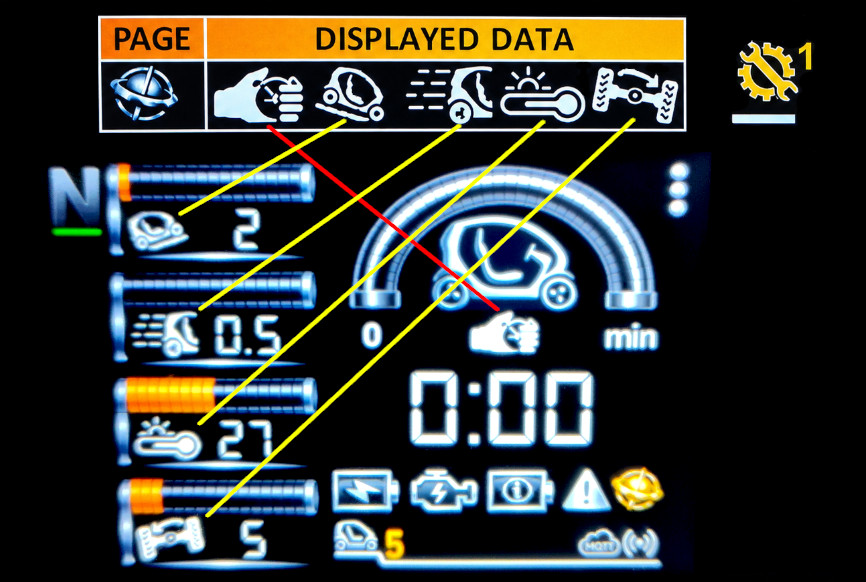
\includegraphics[width=0.8\textwidth]{figures/settings_page1_matching.jpg}
    \caption{Resulting layout values.}
    \label{fig:icon_arrangement}
\end{figure}

After you have customized the shown values \textbf{remember to save by pressing the exit button}.
The new configuration will result as shown in the figure: the first data will be the one
displayed in the foreground at the center of the page, while all the other ones will be
listed in the left side table in the order you specified in the settings page.

\subsubsection{Choosing the starting page}

You can choose which page will be the first one to show when you leave the dashboard page.
To do that press the icon to cycle through all available pages until you find the one you want.
Remember that this configuration is ignored in ToM+ because the dashboard page
will always be the displayed starting one. So, this only work for standard ToM.\\

In the image below the user has selected the battery page, so when leaving the dashboard page ToM+ will show it first.\\

\begin{figure}[H]
    \centering
    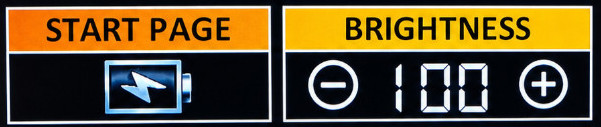
\includegraphics[width=0.7\textwidth]{figures/settings_page1_bright.jpg}
    \caption{Customizing start page and brightness.}
\end{figure}

\subsubsection{Adjusting display brightness}

As you can see in the image above, you can adjust the display brightness by pressing on the \texttt{-} or \texttt{+} buttons.
The brightness can be set from 0 to 100\% and the change will be applied immediately.\\

\subsubsection{Enable/Disable the charging page}

ToM+ has a specific page to display more specific charging data (Section~\ref{sec:charging_page}). You can choose
whether to keep it enabled (\textit{trust me, it's worth it!}) or disabled.


Tap or slide the button on the left to choose between ON and OFF.~When the sliding button is
set to ON the ToM will boot up and load the charging page when your Twizy is
charging otherwise, in the OFF state it will be switched off while charging. To save
your edits press the bottom right corner exit button.\\

\begin{figure}[H]
    \centering
    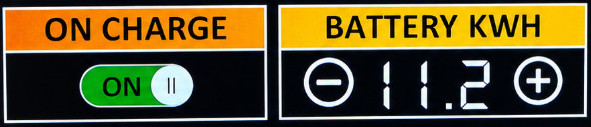
\includegraphics[width=0.7\textwidth]{figures/settings_page1_charge.jpg}
    \caption{Customizing charging page and battery kWh.}
\end{figure}

\subsubsection{Setting your battery capacity}

You can set your battery capacity in kWh, which is useful if you have a Twizy with a
different battery than the standard one. This will help ToM+ to calculate the 
remaining range more accurately. You can adjust the value by 0.1 kWh steps by pressing on 
the \texttt{-} or \texttt{+} buttons, and the change will be applied immediately.
Make sure to \textbf{save your new configuration} by pressing the bottom right corner exit button.

\subsubsection{Calibrating gyroscope module}

If you figure out that gyroscope inclination data could be possibly wrong try pressing
the “CALIBRATE” button which will perform a gyroscope calibration. Make sure
you are \textbf{on a plain surface} with your Twizy before doing this operation otherwise
your inclination data would be even worse. The process is shown down here:

\begin{figure}[H]
    \centering
    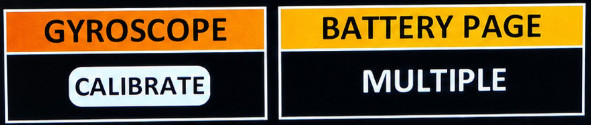
\includegraphics[width=0.7\textwidth]{figures/settings_page1_calibrate.jpg}
    \caption{Adjusting gyroscope calibration.}
\end{figure}

\subsubsection{Changing battery page mode}

You can choose whether to have the condensed battery info page only (Section~\ref{sec:condensed_binfo}) when you press the battery info button or not.

The two available options are \textit{'Condensed'} and \textit{'Multiple'} and you can switch
between them by pressing on the text. The change will be applied as soon as you press the bottom right corner exit button.
\textbf{Multiple} mode will show all the four battery pages we discussed in Section~\ref{sec:condensed_binfo},
while \textbf{Condensed} mode will show only the condensed page.\\

\subsection{Second settings page}

This second settings page is about some advanced settings about the charging process. 
To access it press the circled button in the top right corner of the first settings page and
press it again to navigate to the first settings page.\\

\begin{figure}[H]
    \centering
    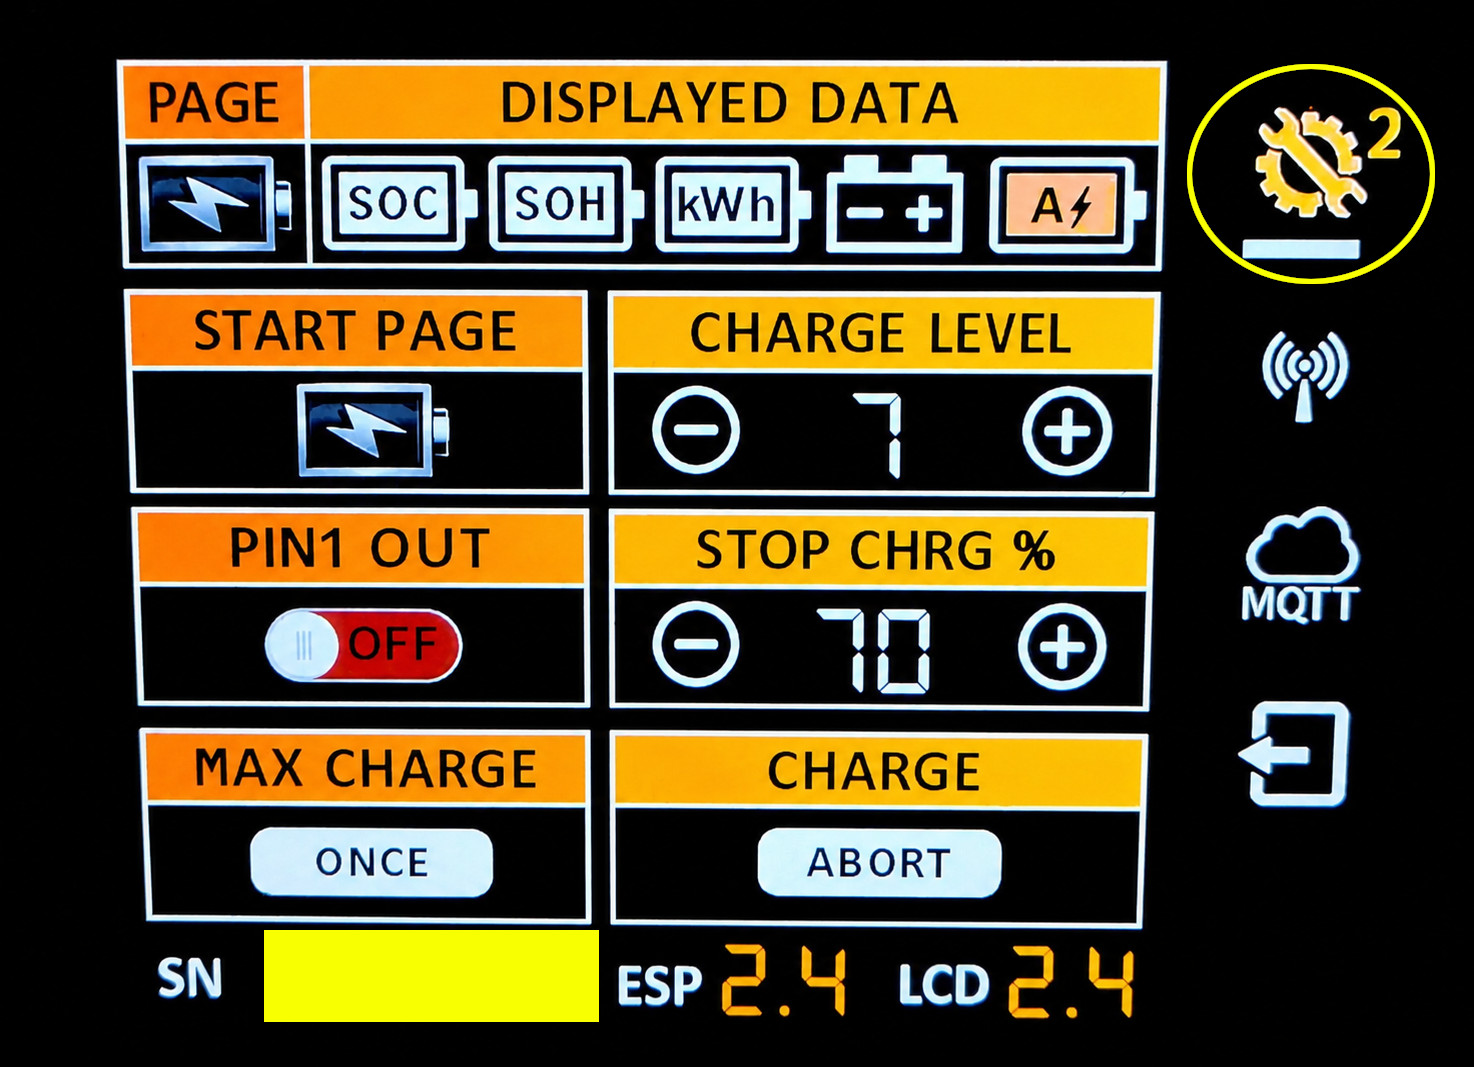
\includegraphics[width=0.8\textwidth]{figures/settings_page2.jpg}
    \caption{Second settings page.}
\end{figure}

\subsubsection{Changing charge level}

You can choose the maximum charge level of your Twizy battery, which is useful if you want to
limit the power absorbed by the battery to increase its lifetime or for other purposes.
The level \textit{'0'} means the limiter is disabled, while the level \textit{'1'} to \textit{'7'} means will use the
corresponding charge level up to the maximum available. 

To increase or decrease the level press on the \texttt{-} or \texttt{+} buttons.
The change will be applied to the current charge if already charging or to the next charge if not.\\

\begin{figure}[H]
    \centering
    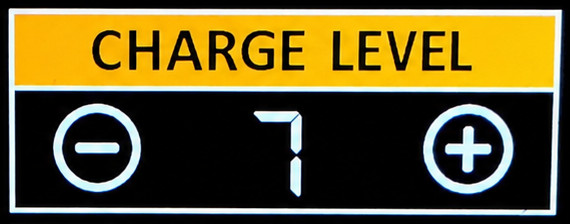
\includegraphics[width=0.5\textwidth]{figures/settings_page2_lvl.jpg}
    \caption{Changing charge level.}
\end{figure}

\subsubsection{Manual control of expansion PIN1}

Some users reported that would be useful to have a manual control of the expansion PIN1, which is normally used to control
an auxiliary charger. So, when needed, you can manually control the expansion PIN1 by pressing the ON/OFF button.
The change will be applied as soon as you press the bottom right corner exit button.\\

\begin{figure}[H]
    \centering
    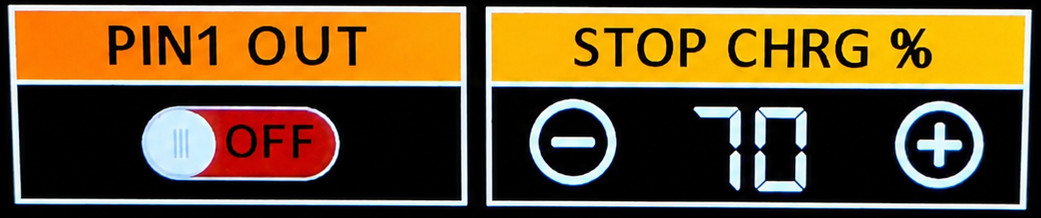
\includegraphics[width=0.7\textwidth]{figures/settings_page2_stop.jpg}
    \caption{Manual control of expansion PIN1 and stop charge level.}
\end{figure}

\subsubsection{Stopping the charge at a specific SOC}

You can choose to stop the charge at a specific SOC, which is useful if you want to
increase the battery lifetime. You can set the value from 0 to 100\% by pressing on the \texttt{-} or \texttt{+} buttons.
The change will be applied to the current charge if already charging or to the next charge if not.\\

\subsubsection{Making a max parameters charge}

You can choose to make a charge with no power and SOC limits, which is useful if you want once in a while
to balance the battery cells. You can press the button to start the max parameters charge,
which will be applied to the current charge if already charging or to the next charge if not.\\

\begin{figure}[H]
    \centering
    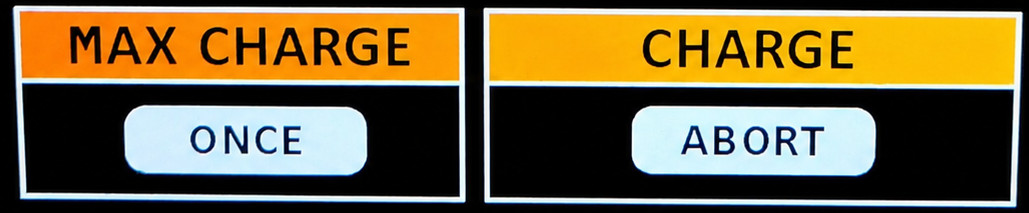
\includegraphics[width=0.7\textwidth]{figures/settings_page2_max.jpg}
    \caption{Max parameters charge and abort charging process.}
\end{figure}

\subsubsection{Abort charging process}

You can choose to abort the charging process, which is useful if you want to stop the charge immediately.
You can press the button to abort the charge, which will be applied instantly.\\

\clearpage

\subsection{The right side menu}

\iconbox{icons/SetupRed1.png}
{Settings page (1 or 2)}
{Shows in which settings page you are. Click to switch.}

\iconbox{icons/WifiBianco.PNG}
{WiFi settings page}
{Change page to the WiFi settings. (Section~\ref{sec:wifi_settings})}

\iconbox{icons/MQTTBianco.PNG}
{MQTT settings page}
{Change page to the MQTT settings. (Section~\ref{sec:MQTT})}

\iconbox{icons/ExitIcon2.png}
{Save and exit button}
{Save changes and exit to the last page.}